\documentclass{article}
\usepackage{amsmath}
\usepackage[utf8]{inputenc}
\usepackage{amssymb,tabu}
\usepackage{array}
\usepackage{float}
\usepackage{enumerate}% http://ctan.org/pkg/enumerate
\usepackage{amsthm}
\newtheorem{theorem}{Theorem}

\usepackage{parskip}
\usepackage{graphicx}
\usepackage{hyperref}
\hypersetup{
  colorlinks,
  citecolor=black,
  filecolor=black,
  linkcolor=black,
  urlcolor=black
}
\usepackage{tikz} 
\theoremstyle{definition} \newtheorem*{definition}{Definition}
\newtheorem{lemma}[theorem]{Lemma}
\newtheorem{proposition}[theorem]{Proposition}
\newtheorem*{corollary}{Corollary} \newtheorem*{remark}{Remark}
\newtheorem*{exmp}{Example} \newtheorem*{exmps}{Examples}
\newtheorem*{obvs}{Observation}
\newtheorem*{warning}{Warning}
\newtheorem*{claim}{Claim}
\newtheorem*{fact}{Fact}

% Isomorphism symbol with function on top
\newcommand{\ts}{\textsuperscript}
\newcommand{\B}{\mathcal{B}}
\newcommand{\myiso}[1]{\stackrel{\mathclap{\normalfont\mbox{#1}}}{\cong}}
\newcommand{\dtn}{\Delta_n} \newcommand{\gene}[1]{\langle #1 \rangle}
\newcommand{\nsg}[2]{#1 \trianglelefteq #2} \newcommand{\func}[3]{#1 : #2
\rightarrow #3} \newcommand{\integers}{\mathbb{Z}}
\newcommand{\reals}{\mathbb{R}} \newcommand{\rationals}{\mathbb{Q}}
\newcommand{\naturals}{\mathbb{N}} \newcommand{\complexes}{\mathbb{C}}
\newcommand{\but}[2]{#1 \backslash \{#2\}} \newcommand{\A}{\mathcal{A}}
\newcommand{\ism}{\cong} \newcommand{\elemt}[2]{#1_{{#2}\sigma(#2)}}
\renewcommand{\vec}[1]{\mathbf{#1}}
\newcommand{\Det}[1]{|#1|}
\newcommand{\CHT}{Cayley-Hamilton Theorem}
\newcommand{\mt}{m_T}
\newcommand{\ct}{c_T}

\DeclareMathOperator{\sgn}{sgn} \DeclareMathOperator{\id}{id}
\DeclareMathOperator{\Span}{Span} 
\DeclareMathOperator{\diag}{diag} 
\DeclareMathOperator{\Orb}{Orb} \DeclareMathOperator{\Stab}{Stab}
\DeclareMathOperator{\Ima}{Im} \DeclareMathOperator{\Sym}{Sym}
\DeclareMathOperator{\lcm}{lcm} \DeclareMathOperator{\hcf}{hcf}
\DeclareMathOperator{\fix}{fix} \DeclareMathOperator{\ord}{\text{ord}}

\title{Algebra II} \author{John R. Britnell - 655\\ Problems class: Wednesday
2:00pm\\ Office hour: Mon 2:00pm} \date{October 2015}

\begin{document}

\maketitle

\tableofcontents \newpage

\section{Groups} 
A group is a set $G$ with a binary
operation $*$ such that \begin{itemize} \item Associativity: $(x * y)*z = x *
    (y * z)$ for all $x,y,z \in G$.  \item Identity: There is $e \in G$ such
      that $e * x = x * e$ for all $x \in G$.  \item Inverses: For all $x \in
        G$ there exists $y \in G$ such that $x * y = yz * y = e$\\
    \end{itemize}

\begin{exmps}\hfill \begin{enumerate}[(i)] \item \begin{itemize} \item
            $\mathbb{Z}_n$, integers modulo $n$ under $+$.  \item $\mathbb{Z}$,
            integers under $+$.  \end{itemize} These are \emph{cyclic groups}.
      \item \begin{itemize} \item $D_{2n}$, $n \geq 3$ dihedral group (of
            rotations and reflections) of a regular $n$-gon.  \item We also
              have $D_\infty$ the \emph{infinite dihedral group}.

Take the ``polygon''.

What are the ``rotations''? These are shifts: move each vertex some number $k$
of places to the right. (if $k$ is -ve we shift left instead). 

``Reflections'' really are reflections - through a vertical axis, either
through a vertex or the midpoint of an ``edge''.

The ``rotations'' and ``reflections'' form a group under composition. This is
$D_\infty$. The subgroup of rotations is an infinite cyclic group, generated by
$R_1$

\end{itemize} \item Symmetric groups $S_n$. Permutations of $\{1, \ldots, n\}$
  under composition. $|S_n| = n!$ More generally if $\Omega$ is a set then
  $\Sym(\Omega)$, the symmetric group on $\Omega$ is the group of all
  permutations of $\Omega$.

\item Let $F$ be a field. Then $GL_n(F)$, the \emph{General Linear Group of
  degree $n$ over $F$}, is the set of \emph{invertible} $n \times n$ matrices
  with entries from $F$. It is a group under matrix multiplication.
  \end{enumerate}
  
\end{exmps}

\subsubsection*{Motivating Example}

\begin{table}[h] \centering $\begin{tabu}{l|llllll} S_3   & e     & (123) &
    (132) & (12)  & (13)  & (23)  \\ \hline e     & e     & (123) & (132) &
    (12)  & (13)  & (23)   \\ (123) & (123) & (132) & e     & (13)  & (23)  &
    (12)   \\ (132) & (132) & e     & (123) & (23)  & (12)  & (13)   \\ (12)  &
    (12)  & (23)  & (13)  & e     & (132) & (123)  \\ (13)  & (13)  & (12)  &
    (23)  & (123) & e     & (132)  \\ (23)  & (23)  & (13)  & (12)  & (132) &
    (123) & e      \\ \end{tabu}$ \end{table}

Now I want to do the Cayley table for $D_6$. We define $R$ to be the rotation,
and $U, V, W$ to be the reflections of the triangle: Then the table is:

\begin{table}[h] \centering $\begin{tabu}{l|llllll} D_6    & e      & R      &
    R^{-1} & U      & V      & W      \\\hline e      & e      & R      &
    R^{-1} & U      & V      & W      \\ R      & R      & R^{-1} & e      & V
    & W      & U      \\ R^{-1} & R^{-1} & e      & R      & W      & U      &
    V      \\ U      & U      & W      & V      & e      & R^{-1} & R      \\ V
    & V      & U      & W      & R      & e      & R^{-1} \\ W      & W      &
    V      & U      & R^{-1} & R      & e \end{tabu}$ \label{tab:cayleyd6}
\end{table} These tables coincide if we make the equivalence: $$ \begin{matrix}
  e      &\longleftrightarrow&  e \\ R      &\longleftrightarrow&  (123) \\
  R^{-1} &\longleftrightarrow&  (132) \\ U      &\longleftrightarrow&  (12) \\
  V      &\longleftrightarrow&  (13) \\ W      &\longleftrightarrow&  (23) \\
\end{matrix} $$

From an algebraic point of view these two groups are ``the same''. We say they
are \textit{isomorphic}.  \subsection{Isomorphisms} Here's a formal definition.\\


\begin{definition} Let $G$ and $H$ be groups, and let $f : G \rightarrow H$ be
a function. We say that $f$ is an \emph{isomorphism} if: \begin{enumerate}[(i)]
  \item $f$ is a bijection.  \item $f(g_1 * g_2)=f(g_1) * f(g_2) $ for all
    $g_1, g_2 \in G$.

note that in $f(g_1 * g_2)$ the multiplication is happening in $g$, but in
$f(g_1) * f(g_2)$ the multiplication is in $h$. if condition (2) is satisfied,
we say that $f$ \emph{respects} $*$.

$G$ and $H$ are \emph{isomorphic} if an isomorphism $G \rightarrow H$ exists.
\end{enumerate} \end{definition}

\begin{itemize} \item $G \overset{f}{\ism} H$ if $G$ and $H$ are isomorphic and
    $f$ is the isomorphism between them.  \item $G \ism H$ if $G$ and $H$ are
    isomorhpic via some isomorphism (particular isomorphism not mentioned)
  \item $G \not\ism H$ if $G$ and $H$ are not isomorphic.\\ \end{itemize}
\begin{exmps} Determine which pairs are isomorphic:

\begin{itemize} \item $S_2=\{e, (1, 2)\}$ \item $\mathbb{Z}_2=\{0,1\}$
    operations: $+\mod 2$ \item $C_2=\{1,-1\}$ operations: multiplication
  \end{itemize} $C_n$ represents $n^{th}$ roots of unity.
  
\end{exmps}

Look at the group tables of the above:

\begin{table}[h] \centering \label{my-label} \begin{tabular}{l|ll} $S_2$  & e
    & (1,2) \\ \hline e     & e     & (1,2) \\ (1,2) & (1,2) & e
  \end{tabular} \end{table}

\begin{table}[h] \centering \label{my-label} \begin{tabular}{l|ll}
    $\mathbb{Z}_2$  & 0  & 1\\ \hline 0     & 0     & 1 \\ 1 & 1 & 0
  \end{tabular} \end{table}

\begin{table}[h] \centering \label{my-label} \begin{tabular}{l|ll} $C_2$  & 1
    & -1\\ \hline 1     & 1  & -1 \\ -1    & -1 & 1    \end{tabular}
\end{table} All groups are isomorphic, which can be shown by ``relabelling'':
\begin{table}[!hp] \centering $\begin{tabu}{rcccl} S_2  &  & \mathbb{Z}_2 & &
    C_2\\ e     & \longleftrightarrow & 0 & \longleftrightarrow & 1 \\ (1,2) &
    \longleftrightarrow & 1 & \longleftrightarrow & -1    \end{tabu}$
  \label{tab:relabelling} \end{table}


Are $\mathbb{Z}_3=\{0,1,2\}$ and $C_3=\{1,w,w^2\}$, where $w=e^{\frac{2\pi
i}{3}}$ isomorphic?

\textbf{Yes}, an isomorphism is: \begin{equation*} f : \left\{ \begin{matrix} 0
    & \mapsto & 1 \\ 1 & \mapsto & w \\ 2 & \mapsto & w^2 \\ \mathbb{Z}_3 &
    \mapsto & C_3 \end{matrix} \right.  \end{equation*}

Another: \begin{equation*} \hat{f} : \left\{ \begin{matrix} 0 & \mapsto & 1 \\
    1 & \mapsto & w^2 \\ 2 & \mapsto & w \\ \end{matrix} \right.
\end{equation*}
 
\begin{remark}\hfill \begin{enumerate}[(i)] \item Let $G$ be finite and let $G \ism
        H$ then $|G|=|H|$ i.e. sets are the same size, clearly since
      isomorphism is a bijection.  \item Let $G$ have identiy $e_G$ and $H$
        have identity $e_H$. Suppose $G \ism H$. Then, $f(e_G)=e_H$.  \item
        `$\ism$' is an is an equivalence relation on groups.  We have symmetry,
      hence order does not matter for isomorphism: \begin{itemize} \item$G \ism
            G $ \textbf{(Reflexivity)} \item$G \ism H \iff H \ism G$
            \textbf{(Symmetry)} \item $G \ism H, H \ism H \implies G \ism K $
              for all groups $G,H,K$\textbf{ (Transitivity)}\\ \end{itemize}
      \end{enumerate} \end{remark}

\begin{exmp} Which of these pairs of groups are isomorphic?  \begin{itemize}
      \item $G_1 = C_4$ = $\{1,-1,i,-i\}$ \item $G_2 = $ group of
        \emph{symmetrics} (rotations and reflections) of a rectangle.\\
        Reflections: $T_x, T_y$, Rotations: $I, R_\pi$ \item $G_3 = $ Rotation
          subgroup of $D_8$.  \end{itemize}
  
Check $G_1 \ism G_3$.  \end{exmp}

\textbf{Note:} $G_1, G_3$ are cyclic groups of order 4. Let $a \in D_8$ be a
rotation of order 4.  Then $G_3 = \{e,a,a^2, a^3\}$.\hfill\\

Define a map $f:G_1 \rightarrow G_3$ by 

\begin{equation*} \begin{matrix} f(1)=e & f(-1) = a^2 \\ f(i)=a & f(-i) = a^3
  \end{matrix} \label{} \end{equation*}

\textbf{Note:} $f(i^n) = a^n$ for all $n \in \mathbb{Z}$

We can see $f$ is a bijection.

And: \begin{align*} f(i^ni^c) &= f(i^{n+c})\\ &= a^{n+c} \\ &= a^n a^c \\ &=
  f(i^n)f(i^c) \end{align*}

Hence, $f$ \emph{respects} multiplication so $G_1 \ism G_3.$\\
\begin{proposition} Let $G$ and $H$ be groups.  \begin{enumerate}[(i)] \item If $|G|
        \neq |H|$ then $G$ and $H$ are not isomorphic \item If $G$ is abelian
          and $H$ is not abelian then $G \not\ism H$ \item If there exists $k
            \in \mathbb{N}$ such that $G$ and $H$ have disjoint numbers of
            elements of order $k$, then $G \not\ism H$ \end{enumerate}
      \end{proposition}

\textbf{Warning:} There does exist pairs of groups $G, H$ which passes the
three above checks but which are not isomorphic.

\begin{proof}\hfill \begin{itemize} \item Any isomorphism is a bijection.
        \item Hwk 1: if $f : G \rightarrow H$ is an isomorphism then $f(g_1)$
        commutes with $f(g_2) \iff g_1$ commutes with $g_2$ $\forall g_1,g_2
      \in G$ \item Hwk 1: If $f:G\rightarrow H$ is an isomorphism then
        $\ord(f(g))=\ord(g)$ $\forall g\in G$ \end{itemize} \end{proof}

\begin{exmps}\hfill \begin{enumerate}[(i)] \item $G=S_4, H=D_8$ - Disjoint orders so
        not isomorphic.  \item $G=S_3, H=C_6=\{1,w,\ldots,w^5\}$ where
        $w=e^{\frac{2 \pi i}{6}}$\\ $H$ is abelian, but $G$ is not, so not
      isomorphic.  \item $G=C_4=\{1,i,-1,-i\}$, $H=\{I,R_\pi,T_x,T_y\}$ \\(the
        symmetry group of a rectangle). \\ Orders of $G$ are 1,4,2,4, but the
        orders of $H$ are 1,2,2,2. We have disjoint numbers of order 2,4, so
        not isomorphic.  \item $G=(\mathbb{R}, +)$, $H=(\but{\reals}{0},
          \times).$\\ -1 is an element of order 2 in $H$ but $G$ has no
          elements of order 2. Therefore not isomorphic.\\ \end{enumerate}
    \end{exmps}

\begin{proposition}\hfill \begin{enumerate}[(i)] \item Let $G$ be a cyclic group of
        order $n$. Then $G \ism \mathbb{Z}_n$ \item Let $G$ be an infinite
          cyclic group. Then $G \ism \mathbb{Z}$.  \end{enumerate}
    \end{proposition}

\begin{proof}\hfill \begin{enumerate}[(i)] \item Let $G=\langle g \rangle$, where
          $G$ has order $n$. Define a map $f : \mathbb{Z}_n \rightarrow G$ by
          $$f(i)=g^i \quad \text{for } i=0,\ldots,n-1$$ Clearly $f$ is a
          bijection.  \begin{enumerate}[(i)] \item Suppose that $i+j<n$ for $i,j \in
              \{0,\ldots,n-1\}.$ 
            
              Then $f(i+j)=g^{i+j}=g^i g^j = f(i)f(j)$.
            \item Suppose that $i+j \geq n$. 
              
              Then, $i+j = i+j-n$ in  $\mathbb{Z}_n$ and $i+j-n \in \{0,\ldots,n-1\}$ so
              $f(i+j)=f(i+j-n)=g^{i+j-n}=g^{i+j}$ (since $g^n=e$).  And this is
            $g^i g^j = f(i) f(j)$.  \end{enumerate} \item Let $G=\langle g
          \rangle$ where $g$ has infinite order. 
          
          Define $f : \mathbb{Z}
          \rightarrow G$ by $f(i)=g^i$ $\forall i \in \mathbb{Z}$. Clearly $f$
          is a bijection and $f(i+j)=g^{i+j}=g^i g^j = f(i) f(j)$.
      \end{enumerate} \end{proof}

\begin{remark} It follows that $\mathbb{Z}_n \ism C_n$ (complex $n^{th}$ roots
  of unity) for all $n$.  \end{remark}

\subsection{Even and odd permutations}

Consider the polynomial $\Delta_3 = (x_1 - x_2)(x_1 - x_3) (x_2 - x_3)$.  Let
$g \in S_3$, and consider the effort of applying $g$ to the variables $x_1,
x_2, x_3$ in $\Delta_3$.

$$g(\Delta_3) = (x_{g(1)} - x_{g(2)})(x_{g(1)} - x_{g(3)})(x_{g(2)} -
x_{g(3)}).$$

\noindent We see that $g(\Delta_3)=I\Delta_3$. More generally, let $$\Delta_n =
\prod_{i<j\leq n} (x_i - x_j ). $$ 

\noindent Then, if $g \in S_n$, we can apply $g$ to $\Delta_n$ by $$g(\Delta_n)
= \prod_{i<j\leq n}(x_{g(i)} - x_{g(j)}).$$

\noindent We have $g(\Delta_n) = \pm\Delta_n$.\\ \begin{definition} The
  \emph{signature} of $g$, $\sgn(g)$, is \begin{align*} +1 \quad \text{ if }
    g(\dtn) &= \dtn \\ -1 \quad \text{ if } g(\dtn) &= -\dtn \end{align*}
\end{definition}

The \emph{parity} of $g$: If $\sgn(g)=+1$, say that $g$ is \emph{even}.  If
$\sgn(g)=-1$, say that $g$ is \emph{odd}.\\

\begin{exmp}
  
In $S_3$, we have that 

$id,\,(1 2 3), (1 3 2)$ are even.

$(1 2),\, (1 3),\,(2 3)$ are odd.\\ \end{exmp} \begin{obvs}
  
The even permutations in $S_3$ form a subgroup (this always happens)\\
\end{obvs}


\begin{proposition} \label{prp:sgn}\hfill \begin{enumerate}[(i)] \item
        $\sgn(gh)=\sgn(g)\sgn(h)$ for all $g,h \in S_n$.  \item
        $\sgn(g^{-1})=\sgn(g)$ for all $g \in S_n$.  \item if $\tau=(i j)$ is a
          2-cycle, then $\sgn(\tau)=-1$.  \end{enumerate} \end{proposition}

\begin{proof}\hfill \begin{enumerate}[(i)] \item Let $g,h \in S_n$, \begin{align*}
              gh(\dtn) &= g(h(\dtn)) \\ &= g(\sgn(h)\dtn) \\ &=
              \sgn(h)(g(\dtn)) \\ &= \sgn(h) \sgn(g) \dtn \end{align*} So
            \begin{align*} \sgn(gh) &= \sgn(h)\sgn(g) \\ &= \sgn(g)\sgn(h)
            \end{align*}

    \item We have $g g^{-1}=e$, and clearly $\sgn(e) = +1$. 

      So $\sgn(g g^{-1})=\sgn(g)\sgn(g^{-1})=+1$ (by (1)).

      So $\sgn(g^{-1})=\sgn(g)^{-1}$ by (1).

    \item Apply $(ij)(\dtn):$ We count the number $N$ of brackets in $\dtn$
      which are sent by $(ij)$ to things of the form $(x_k - x_i)$ where $k>i$ 

      Then $\sgn\left( (ij) \right)=(-1)^N$

      Count $p,q$. $p<q$, but $(ij)(p)>(ij)(q)$

      Cases: \begin{enumerate}[(i)] \item $i=p,\, j=q$ - (1 possibilty) \item
          $p=i,\,q<j$ - possibilities $q \in \left\{ i+1, \ldots, j-1 \right\}$
        \item $i<p,\,q=i$ - possibilities $p \in \left\{ i+1, \ldots , j-1
          \right\}$ \end{enumerate} So there are $2(j-i-2) +1$ possibilities in
      total.

      So $N=2(j-i-2)+1$ is odd. 

      Hence, $\sgn\left( (ij) \right)=-1$ \end{enumerate} \end{proof}

\begin{proposition} \label{prp:2cycles} Let $c=(a_1 \ldots a_r)$ be an
  $r$-cycle. Then $c$ is a product of $r-1$ 2-cycles.  \end{proposition}

\begin{proof} Easy to check that
  $$c=(a,a_n)\ldots(a,a_5)(a,a_4)(a,a_3)(a,a_2).$$ \end{proof}

\begin{corollary} An $r$-cycle is even when $r$ is odd and even when $r$ is
  even.\\ \end{corollary}

\begin{proposition}\hfill \begin{enumerate}[(i)] \item Every permutation can be
        written as a product of 2-cycles.  \item If $g$ is a product of
          disjoint cycles of lengths $r_1, \ldots, r_k$

      Then the signature of $g$ is $\prod_{i} (-1)^{r_i - 1}$ \end{enumerate}
\end{proposition}

\begin{proof} We saw last year that any permutation is a products of disjoint
  cycles.

  Each of the cycles is a product of 2-cycles by Prop. \ref{prp:2cycles} and so
  $g$ is too.

  (2) Follows from Prop. \ref{prp:2cycles} and Prop. \ref{prp:sgn}.1.
\end{proof}

Rule of thumb:

A permutation is even if it has an even number of cycles of even length.

It is odd if it has an odd number of cycles of even length.\\

\begin{exmp} $$(1 2 3 4)(6 7 9)(8 4 10) \in S_{10}$$ is odd (one cycle of even
  length) \end{exmp}


\subsection{Alternating Groups}

Define $A_n=\left\{ g \in S_n | \sgn(g) = +1 \right\}$ (The even permutations
in $S_n$).\\

\begin{theorem} Let $A_n$ is a subgroup of $S_n$. If $n>1$, then
  $|A_n|=\frac{1}{2}n!$ \label{thm:subgroup} \end{theorem}

\begin{proof} $A_n$ is non-empty since it contains $e$. $A_n$ is closed under
  the group operation by Prop. \ref{prp:sgn}.1 and under inverses by Prop.
  \ref{prp:sgn}.2.

  Consider the coset $(12) A_n$. We know this coset has the same size as $A_n.$
  Since $(1 2)$ is odd, we have \begin{equation*} A_n \cap (1 2) A_n  =
    \emptyset \end{equation*}

I claim that $A_n \cup (1 2) A_n $ is $S_n$. 

Let $g \in S_n$.

If $\sgn(g) = +1$ then $g \in A_n$.  If $\sgn(g) = -1$ then $\sgn\left( (12) g
\right)= +1$.

So $(12)g \in A_n$

But $(1 2)\left( (1 2) g \right)=g$, and so $g \in (1 2)A_n$.

Hence, $|A_n|=\frac{1}{2}|S_n|=\frac{1}{2}n!$

\end{proof}

\textbf{Examples:}\\ $A_2 = \{ id \}$, $A_3 = \{id, (123), (132)\}$.

What about $A_4$? We know that $|A_4|=\frac{1}{2}4!=12$.

The cycle structures in $S_4$ are: $(1,1,1,1)$ - 1 element, $(2,2)$ - 3
elements, $(3,1)$ - 8 elements.  $A_5$ has order $\frac{1}{5}5! = 60$.

The even cycle shapes are: $(1,1,1,1,1)$ - 1 element, $(2,2,1)$ - 15 elements,
$(3,1,1)$ - 20 elements, $(5)$ - 24 elements. These four numbers add up to 60.

\emph{Exercise:} Do this for $A_6$.

\subsection{Direct products} Recall that if we have set $X_1, \ldots, X_n$, the
Cartesian product $X_1 \times X_2 \times \ldots \times X_n$ is the set of
tuples $\{(x_1, \ldots,x_n) : x_i \in X_i\}$

What if the sets are actually groups?

Let $G_1 , \ldots, G_n$ be groups. Then we can define a binary operation on
their Cartesian Product by $$(g_1, \ldots, g_n) * (h_1, \ldots , h_n) =
(g_1h_1, g_2h_2, \ldots, g_nh_n).$$ \begin{proposition} Under this binary
  operation, $G_1 \times \ldots \times G_n$ is a group. This is called the
  \textit{direct product} of $G_1 , \ldots, G_n$.  \end{proposition}

\begin{proof} Check the group axioms: \begin{itemize} \item
          \textbf{Associativity:} \begin{align*} & ((g_1, \, \ldots \, ,
            g_n)(h_1,\, \ldots, \, h_n)) (k_1, \, \ldots , \, k_n) & \\ &= (g_1
            h_1, g_2 h_2, \ldots, g_n h_n) (k_1, \ldots , k_n) & \\ &= ((g_1
            h_1)k_1, \ldots , (h_n h_n)k_n), & \text{each } G_i \text{
            associative}\\ &= (g_1, \ldots, g_n) (h_1 k_1, \ldots, h_n k_n) &
            \\ &= (g_1, \ldots, g_n) ((h_1, \ldots, h_n) (k_1, \ldots, k_n)) &
        \end{align*} \item \textbf{Identity:}

Let $e_i$ be the identity of $G_i$ for all $i$. Then $(e_1, \ldots, e_n)$ is an
identity for $G_1 \times \ldots \times G_n$ \item \textbf{Inverses:}

The element $(g_1, \ldots , g_n)$ has the inverse $(g_1^{-1}, \ldots
g_n^{-1})$.

\end{itemize}

\end{proof} \emph{Example}: Consider the group $C_1 \times C_2$ which has
elements $(1,1), (1,-1),(-1,1),(-1,-1)$

\begin{table}[h] \centering \label{my-label} $\begin{tabu}{l|llll} & e & a & b
    & c \\ \hline e & e & a & b & c \\ a & a & e & c & b \\ b & b & c & e & a
    \\ c & c & b & a & e \end{tabu}$ \end{table}

Recall the group of symmetries of the rectangle, $\{I, R_\pi, T_x, T_y\}$.

This has group table:

\begin{table}[h] \centering \label{my-label} \begin{tabular}{l|llll} & I      &
    $R_\pi$ & $T_x$   & $T_y$   \\ \hline I      & I      & $R_\pi$ & $T_x$   &
    $T_y$   \\ $R_\pi$ & $R_\pi$ & I      & $T_y$   & $T_X$    \\ $T_x$   &
    $T_x$   & $T_y$   & I      & $R_\pi$ \\ $T_\pi$ & $T_y$   & $T_x$   &
    $R_\pi$ & I     \end{tabular} \end{table}

So we have an isomorphism given by

$e \rightarrow I$\\ $a \rightarrow R\pi$\\ $b \rightarrow T_x$\\ $c \rightarrow
T_y$\\

Recall from M1P2 that $S_4$ has a subgroup $$\{id,  (12)(34)=x, (13)(24)=y,
(14)(23)=z\}.$$

This has the above group table.  \begin{table}[!ht] \centering
  $\begin{tabu}{l|llll} & id & x  & y  & z \\ \hline id & id & x  & y  & z \\ x
    & x  & id & z  & y \\ y  & y  & z  & id & x \\ z  & z  & y  & x  & id
  \end{tabu}$ \end{table}

This is also isomorphic to $C_2 \times C_2$, via $e \rightarrow id, a
\rightarrow x, b \rightarrow y, c \rightarrow z$.\\

\begin{exmp}
  
$C_2 \times C_2 \times C_2$, which has elements $(\pm 1, \pm 1, \pm 1)$. We see
there are 8 elements and $x^2=(1,1,1)=e$ for any $x$.\\ \end{exmp}

\begin{proposition}\hfill \label{prp:ordgroup} \begin{itemize} \item $|G_1
        \times \ldots \times G_n| =|G_1||G_2|\ldots|G_n|.$ \item If \emph{all}
          of the groups $G_i$ are abelian, then so is $G_1 \times \ldots \times
          G_n$. But if \emph{any} of $G_1, \ldots G_n$ is not abelian then
          netiher is $G_1 \times \ldots \times G_n$.  \item Let $(g_1, \ldots
            g_n) \in G_1 \times \ldots \times G_n$. Then $\ord (g_1, \ldots ,
            g_n) = \lcm (\ord g_1, \ldots , \ord g_n)$.  Proof not known.
        \end{itemize} \end{proposition}

\begin{proof}\hfill \begin{enumerate}[(i)] \item We know from set theory that $|A
          \times B| = |A| \times |B|$ (for sets $A,B$). An easy induction shows
          that $|A_1 \times A_2 \times \dots \times A_n| = |A_1| \times |A_2|
          \times \dots \times |A_n|$.  \item Suppose that $G_1, \dots , G_n$
            are all abelian. For all $i$, let $g_i,h_i\in G_i$. Then
            $g_ih_i=h_ig_i$. Take $g,h \in G_1 \times \dots \times G_n$, say
            $g=\left( g_1, \dots , g_n \right)$, $h = \left( h_1, \dots , h_n
            \right)$. Now \begin{align*} gh &= \left( g_1 h_1, \dots , g_n h_n
              \right)\\ &= \left( h_1g_1, \dots , h_n g_n \right)\\ &= hg
            \end{align*}

For the converse, suppose that $G_i$ is not abelian for some $i$. Then there
exists $g_i,h_i \in G$ such that $g_ih_i \neq h_ig_i$. Define $g,h \in G_1
\times \dots \times G_n$ by $g = \left( e_1,\dots e_{i-1},g_ie_{i+1},\dots,e_n
\right)$ and $h = \left( e_1, \dots e_{i-1},h_i,e_{i-1},\dots,e_n \right)$
where $e_j$ is the identity of $G_j$ (or $H_j$ respectively) for all $j$. Now

\begin{align*} gh &= \left( e_1,\dots,e_{i-1},g_ih_i,e_{i+1},\dots,e_n
  \right)\\ hg &= \left( e_1,\dots,e_{i-1},h_ig_i,e_{i+1},\dots,e_n \right)
\end{align*}

So $gh \neq hg$, since they differ in the $i$th coordinate.

\item Let $g_i \in G_i$ and let $\ord g_i=h_i$ for all $i$. Let
  $m=\lcm(k_1,\dots k_n)$.

  \textbf{Fact:} $(g_1, \dots ,g_n)^{k}=(g_1^k,\dots,g_n^k)$ for all $k \in
  \integers$. (Proof: \emph{Exercise}).

  By this fact, we have \begin{align*} \left( g_1, \dots, g_n \right)^m &=
    \left( g_1^m, \dots,g_n^m \right)\\ &= \left( e_1, \dots,e_n \right)
  \end{align*} Since $k_i | m$ for all $i$.

  Suppose that $l<m$, ($l>0$). Since $m$ is the \emph{least} common multiple of
  $k_1, \dots, k_n$, we must have that $k_i\nmid l$ for some $i$. So $g_i^l\neq
  e_i$. Hence $\left( g_1^l,\dots,g_n^l \right) \neq \left( e_1,\dots,e_n
  \right)$, since they differ in coordinate $i$. So $\left( g_1 ,\dots,g_n
  \right)^l \neq \left( e_1, \dots,e_n \right)$. Hence $\ord \left( g_1
  ,\dots,g_n \right)=m$, as required.  \end{enumerate} \end{proof}

\begin{exmp} All cyclic groups are abelian, so any direct product of cyclic
  groups is abelian. For example $C_4 \times C_2$ and $C_2 \times C_2 \times
  C_2$ are ``new'' abelian groups of order 8.

  Note that these are not isomorphic, and neither of them is isomorphic to
  $C_8$. $C_8$ has an element of order 8. $C_4 \times C_2$ has an element
  $(i,-1)$ of order 4 but no element or order 8.  $C_2 \times C_2 \times C_2$
  has no element of order $> 2$.

\end{exmp} \emph{What about $C_2 \times C_4$?}

  \textbf{Observation:} For any groups $G,H$ we have $G \times H \ism H \times
  G$. An isomorphism is given by $(g,h)\mapsto (h,g)$ (routine check), so $C_2
  \times C_4 \ism C_4 \times C_2$.\\

  \begin{proposition} \label{prp:hcfcyclic} Let $m,n \in \naturals$ be such
    that $\hcf(m,n)=1$. Then $C_m \times C_n \ism C_{mn}$.  \end{proposition}

  \begin{proof} Let $C_m = \gene{g}$, $C_n=\gene{h}$. Then $\ord(g)=m$ and
    $\ord(h)=n$. So $\ord(gh)$ is $\lcm(m,n)$ by Prop. \ref{prp:ordgroup}.3.
    But $\lcm(m,n)=mn/\hcf(m,n)$ and this is $mn$ since $\hcf(m,n)=1$. So $C_m
    \times C_n$ has an element $(h,g)$ of order $mn$, so it is cyclic. Hence
    $C_m \times C_n \ism C_{mn}$.\\ \end{proof} 

  \begin{theorem}(Fundamental Theorem of Finite Abelian Groups)\hfill\\ Every
    finite abelian group is a direct product of cyclic groups.
    \label{thm:funda} \end{theorem}

  \begin{proof} Omitted.  \end{proof}

  \begin{exmps}\hfill \begin{enumerate}[(i)] \item There is only one abelian group
            (up to isomorphism) of order 6. The only factorisations of 6 are 6,
            $3 \times 2$. So the only direct proposition of cyclic groups which
            have order 6 are $C_6$ and $C_3 \times C_2$. But these are
            isomorphic by Prop. \ref{prp:hcfcyclic}.  \item There are exactly
              three abelian groups of order 8 - those listed above.
          \end{enumerate} \end{exmps}

\subsection{Small groups} \begin{enumerate}[(i)] \item Every group of order 1 is
    isomorphic to $\{1\}$.  \item Every group of prime order is cyclic, so
      isomorphic to $C_8$. So only one group of order $2,3,5,7,\ldots$

\item Groups of order 4: Certainly we have $C_4$. Any other group must have 3
  elements of order 2, say $a,b,c$. Start our multiplication table:

    \begin{table} 
      $\begin{tabu}{l|llll} 
        & e&a&b&c\\\hline 
        e & e&a&b&c\\ 
        a & a&e& &\\ 
        b & b& &e&\\ 
        c & c& & &e 
      \end{tabu}$
    \end{table}

The six vacant places are all determined by the fact that every element must
appear once in every row and every column.

Complete table: \begin{table}[h] \centering $\begin{tabu}{l|llll} &
    e&a&b&c\\\hline e & e&a&b&c\\ a & a&e&c&b\\ b & b&c&e&a\\ c & c&b&a&e\\
  \end{tabu}$ \label{tab:completesimpletable} \end{table}

So $G \ism C_2 \times C_2$ (So every group of order 4 is abelian).

\item Groups of order 6.

  Certainly we have $C_6$. Any other group has 5 elements with orders 2 or 3,
  with at least one of order 2 (by Prop. \ref{prp:ordgroup})

  \underline{Result:} if a group $G$ has only elements of order $\leq 2$, then
  $G$ is abelian. (If $g^2 = e$ for all $g$, look at $(ab)^2 = e$. So
  $ab\underline{ab}=e$ and also $ab\underline{ba}=aa=e$. By left cancellation,
  $ab=ba$, for all $a,b$

  The abelian groups of order 5 are $C_6, C_2 \times C_3$, which are
  isomorphic. If follows that every group of order 6 hs an element of order 3.

  Let $a$ be an element of order 3.

  Let $b$ be an element of order 2.

  \begin{equation} G = \langle a \rangle \cup b \langle a \rangle \text{ so } G
    = \left\{ e,a,a^2,b,ba,ba^2 \right\} \label{} \end{equation}

  Starting our multiplication table: 
  \begin{table}[H] \centering
    $\begin{tabu}{l|lll|lll} 
      &e   &a   &a^2  & b   &ba   &ba^2\\\hline 
      e &e   &a   &a^2  & b   &ba   &ba^2\\
      a   &a &a^2 &  e\\ 
      a^2    &a^2   &e    &a\\ 
      b   &b &ba  &ba^2& e \\ 
      ba  &ba& ba^2& b\\ 
      ba^2 &ba^2 &b &ba
    \end{tabu}$ 
    \label{tab:multtableincomplete} 
  \end{table}

Note that if $ab=ba$ then we can check that $ab$ must have order 6, since
$(ab)^2=a^2b^2=a^2$, $(ab)^3=a^3b^3=b.$ But $G$ is not cyclic, by assumption,
so $ab\neq ba$.  Hence we must have $ab = ba^2$.

This allows us to complete the multiplication table:

\begin{table}[H] \centering \label{my-label} $\begin{tabu}{l|llllll} & e & a &
    a^2 & b & ba & ba^2    \\ \hline e & e & a & a^2 & b & ba & ba^2    \\ a &
    a & a^2 & e & ba^2 & b & ba    \\ a^2 & a^2 & e & a & ba & ba^2 & b  \\ b &
    b & ba & ba^2 & e & a & a^2    \\ ba & ba & ba^2 & b & a^2 & e & a   \\
    ba^2 & ba^2 & b & ba & a & a^2 & e \end{tabu}$ \end{table}

We can check that  $G$ is isomorphic to $S_3$. So the groups of order 6 are
$C_6$ and $S_3$.

\item Groups of order 8.

  Abelian groups: $C_8,C_4\times C_2, C_2 \times C_2 \times C_2.$ 

  Non abelian group $D_8$.

  There is one other non abelian group.  \begin{equation*} Q_8 = \left\{ \pm1,
    \pm i, \pm j, \pm k \right\} \text{ where } i^2=j^2=k^2=-1.  \label{}
  \end{equation*} \begin{equation*} \begin{matrix} ij=k & jk=i & ki=j \\ ji=-k
      & kj=-i & ik=-j \end{matrix} \end{equation*} This is the \emph{quaternion
  group}.  $Q_8$ has six elements of order 4.  $D_8$ only has two elements of
  order 4, so they are not isomorphic.

  Alternatively, lets define matrices

  \begin{equation*} A = \left( \begin{matrix} 0 & 1 \\ -1 & 0 \end{matrix}
    \right), B = \left( \begin{matrix} i & 0 \\ 0 & -i \end{matrix} \right), C
    = \left( \begin{matrix} 0 & -i \\ -i & 0 \end{matrix} \right) \label{}
  \end{equation*}

  So $A,B,C \in GL_2(\mathbb(C))$. I claim that if $G = \left\{ \pm I, \pm A,
  \pm B, \pm C \right\}$

  Then $G \leq GL_2(\mathbb(C))$ and there is an isomorphism $G \equiv Q_8$
  given by 

  \begin{equation*} \begin{matrix} f(\pm I ) = \pm 1 & f(\pm A) = \pm i \\
      f(\pm B ) = \pm j & f(\pm C ) = \pm k \end{matrix} \label{}
  \end{equation*} It follows that since matrix multiplication is associative,
  the multiplication on $Q_8$ is associative too!

\item All groups of order 9 are abelian, so either $C_9$ or $C_3 \times C_3$.
  The groups of order 10 are $C_{10}$ and $D_{10}$. Groups of order 12 are
  $C_{12}$, $ C_{6} \times C_2$ (the abelian ones), $D_{12},A_{4}$, and one
  other. 

  Groups of order 14 are $C_{14}$ and $D_{14}$. 

  The only group of order 15 is $C_{15}$.

  There are 14 groups of order 16.  \end{enumerate}

Helpful result: \begin{proposition} Let $G$ be a group of even order. Then $G$
  has an element of order 2.  \end{proposition}

\begin{proof} Let $S$ to be the subset of $G$ such that \begin{equation*} S =
    \left\{ g \in G : \ord g > 2 \right\}.  \end{equation*} $g \in S \iff
  g^{-1} \in S$ (Since $\ord g^{-1} = \ord g$). And $g \neq g^{-1}$, since $g^2
  \neq e$. So $S$ contains pairs $(g,g^{-1})$ of elements, so $|g|$ is even. 

  But $|G|=|S| + |\left\{ g : \ord g=2 \right\}| + 1$ (identity). 

  So $|\left\{ g : \ord g = 2 \right\}|=|G|-|S|-1$ which is odd. 

  So $\left\{ g : \ord g = 2 \right\} \neq \emptyset.$

\end{proof}


\subsection{Homomorphisms}

For an isomorphism we had two conditions that a map $G \rightarrow H$ has to
satisfy:

\begin{enumerate}[(i)] \item Bijection \item Respect of multiplication
  \end{enumerate}

If we drop (1), we get the definition of a homomorphism.\\

\begin{definition} A map $f:G \rightarrow H$ is a \emph{homomorphism} if $f(g_1
  g_2)=f(g_1)f(g_2)$ for all $g_1,g_2 \in G.$\\ \end{definition}

\begin{exmps}\hfill \begin{enumerate}[(i)] \item Any isomorphism is a homomorphism.
        In fact an isomorphism is a bijection homomorphism.  \item Let $G,H$ be
          any groups. Then $f : G \rightarrow H$ defined by $f(g) = e_H$ is a
          homomorphism. (Check $f(g_1 g_2)=e_h$, $f(g_1)f(g_2)=e_He_h = e_h$).
          This is the ``trivial homomorphism'' $G \rightarrow H.$ \item Let $G
          \leq H$. Then $f:G\rightarrow H$ defined by $f(g)=g$ is a
        homomorphism. (The inclusion map of $G$ into $H$.) \item Define
          $\text{sign}:S_n \rightarrow C_2$ by
          $\text{sign}(g)=\text{sign}(g)=+1 \text{ if } g $ is even, $-1$ if
          $g$ is odd. (We showed before that $\sgn(gh)=\sgn(g)\sgn(h)$.) \item
            Define $f:D_{2n} \rightarrow C_2$ by 

    $f(g)=1$ if $g$ a rotation, $-1$ if $g$ a reflection.

    This is a homomorphism. (We know rot $\times$ rot $=$ rot, ref $\times$ rot
    $=$ ref, rot $\times$ ref $=$ ref, ref $\times$ ref $=$ rot).

    So its easy to see that $f$ respects multiplication.

  \item Define $f:GL_2(F) \rightarrow F^\times$ by $$F(g) = \text{det}g.$$ Then
  $f$ is a homomorphism.  (We know that
$\text{det}(gh)=(\text{det}g)(\text{det}h)$ for $g,h \in GL_2(F)$.) This can be
done for $n>2$ as well.  \item Let $V,W$ be vector spaces, and let $T:V
  \rightarrow W$ be a linear transformation. Then $V$ and $W$ are groups under
  $+$ and $T$ is a homomorphism (We know that $T(v_1 + v_2)=T(v_1)+T(v_2)$
  since $T$ preserves addition.) \item Define $f: (\mathbb{R},+)\rightarrow
    (\mathbb{C}^\times,\times)$ by $f(x)=e^{2 \pi i x}.$ Then $f$ is a
    homomorphism. (Check: $f(x+y)=e^{2\pi i (x+y)}=e^{2\pi i x}e^{2 \pi i
    y}=f(x)f(y)$).\\ \end{enumerate}
  
\end{exmps}


\begin{proposition} Let $f: G \rightarrow H$ be a homomorphism.
\begin{enumerate}[(i)] \item $f(e_G)=e_H$ \item $f(g^{-1})=f(g)^{-1}$ for all $g \in
    G$.  \item $\ord f(g)$ divides $\ord g$ for all $g \in G$.  \end{enumerate}
\end{proposition}

\begin{proof} (1) and (2) are the same as for the corresponding parts of
  Proposition \ref{prp:sgn}.

  (3) \emph{Claim:} $f(g^k)=f(g)^k$ for all $k\in \mathbb{Z}.$ \begin{proof} If
    $k \geq 0$, use induction. If $k<0$, show instead that $f\left( \left(
    g^{-1} \right)^{-k} \right)=f(g^{-1})^{-k}$. (i.e. replace $g$ with
    $g^{-1}$ and $k$ with $-k$). Now suppose that $k=\ord g$. Then $g^k = e_G$.
    $f(g^k)=f(e_G)=e_H$. Now by the claim, $f(g)^k=e_H$ and so we have $\ord
    f(g)$ divides $k$.  \end{proof} \end{proof}

\begin{definition} Let $f:G \rightarrow H$ be a homomorphism. We define: 
  
  The \emph{image} of $f$: $\text{Im } f = \left\{ f(g) : g \in G \right\}$.

  The \emph{kernel} of $f$: $\text{ker } f=\left\{ g \in G : f(g) = e_H
  \right\}$\\ \end{definition}

\begin{theorem}\hfill \begin{enumerate}[(i)] \item $\text{Im } f$ is a subgroup of
        $H$.  \item $\text{ker } f$ is a subgroup of $G$.  \end{enumerate}
      \label{} \end{theorem}

\begin{proof}\hfill \begin{enumerate}[(i)] \item Check the axioms.

      $f(e_g)=e_H$ so $e_H \in \text{Im }f$.  Suppose $h_1, h_2 \in \text{Im }
      f$. Then there exist $g_1, g_2 \in G$ such that $f(g_1)=h1, f(g_2)=h_2$.
      Now, $f(g_1 g_2)=f(g_1)f(g_2)=h_1 h_2$. So $\text{Im }f$ is closed under
      the group operation.

      Suppose $h \in \text{Im }f. $ Then $h=f(g)$ for some $g \in G$. Now
      $f(g^{-1})=f(g)^{-1}=h^{-1}$. So $\text{Im }f$ is closed under inverses.
      So $\text{Im } f \in H $.

    \item Again, check the subgroup conditions.  $f(e_G)=e_H$, so $e_G \in
      \text{ker }f$. Suppose $g_1, g_2 \in \text{ker }f$. Then
      $f(g_1)=f(g_2)=e_H$. ow $f(g_1 g_2)=f(g_1)f(g_2)=e_He_H=e_h$. So $g_1 g_2
      \in \text{ker }f$. Finally, let $g \in \text{ker }f$. Then $f(g)=e_H$.
      now $f(g^{-1})=f(g)^{-1}=e_H^{-1}=e_H$, so $g^{-1} \in \text{ker }f$. So
      $\text{ker }f \leq G$.  \end{enumerate} \end{proof}

\begin{exmp} Suppose $G=S_3$. Let $f$ be a homomorphism from $G$ to some group
  $H$. What are the possibilities for $\text{Im }f$ and $\text{ker }f$?

  Recall that for $g \in G$ we have $f(g)$ divided $\ord g$.

  In $S_3$ we have elements $(123)$, $(12)$ of orders 3 and 2 respectively. So
\begin{enumerate}[(i)] \item $f\left( (123) \right)$ has order 3 or else $f\left(
    (123) \right)=e_H$ \item $f\left( (12) \right)$ has order 2 or else
      $f\left( (12) \right)=e_H$ \end{enumerate}

  \textbf{Case 1:} $f\left( (123) \right)$ has order 3 and $f\left(
  (12)\right)$ has order 2. In this case $|\text{Im }f|$ is divisible by both 2
  and 3. But $|\text{Im }f| \leq 6$, so we must have $\text{Im } f=6$. So
  (considered as a map $G \rightarrow \Ima f$) $f$ is bijective. Hence $\Ima f
  \cong S_3$.

  \textbf{Case 2:} $f\left( (12) \right)=e_H$. In this case observe that
  $(123)=(13)(12)$.

  So $f\left( (123) \right)=f\left( (13) \right)e_H=f\left( (13) \right)$.

  But $f\left( (123) \right)$ divides 3 and $f\left( (13) \right)$ divides 2.
  Hence these must both be $e_H$. Now we see that $\ker f$ is a subgroup of
  $S_3$ containing $id, (123), (12), (13)$, so $\ker f=S_3$. And so $\Ima f =
  \left\{ e_H \right\}$. $f$ is the trivial homomorphism.

  \textbf{Case 3:} $f\left( (12) \right)$ has order 2, $f\left( (123)
  \right)=e_H$. Notice that $(13)(12)=(123)$, so $f\left( (13) \right)f\left(
  (12) \right)=e_H$. So $f\left( (13) \right)=f\left( (12) \right)^{-1}=f\left(
  (12) \right)$ (Since $f\left( (12) \right)$ has order 2).

  Similarly $(12)(23)=(123)$, so $f\left( (12) \right)=f\left( (23) \right)$.
  Hence the image is $\left\{ e_H,f\left( (12) \right) \right\}$, a group of
  order 2, and $\ker f=\left\{ e,(123),(132) \right\}$.

  If we take $\Ima f$ to be $C_2$, then $f$ is the sign homomorphism.\\
  \begin{obvs}
  
  Not every subgroup of $S_3$ occurred as the kernel of a homomorphism.
\end{obvs} \end{exmp}

The next subsection explores which subgroups can occur.

Suppose $\func{f}{G}{H}$ is a homomorphism, and suppse $g \in \ker f$. Let
$g_1$ be every element of $G$. Then I claim $g_1,g_0,g_1^{-1}\in \ker f$.

Check: \begin{align*} f(g_1\,g_0\,g_1^{-1}) &= f(g_1)f(g_0)f(g_1)^{-1}\\ &=
  f(g_1)e_Hf(g_1)^{-1} \\ &= e_H.  \end{align*}

So if $K=\ker f$, then $K=gKg^{-1}=\left\{ gKg^{-1} : k \in K \right\}$ for all
$g \in G.$\\

\begin{proposition} \label{prp:tfae} Let $G$ be a group and let $H$ be a
subgroup of $G$. The following are equivalent: \begin{enumerate}[(i)] \item
    $H=gHg^{-1}$ for all $g \in G$.  \item $Hg=gH$ for all $g \in G$.  \item
      Every left coset is a right coset \item Every right coset is a left coset
      \item $gHg^{-1} \subseteq H$ for all $g \in G$ \end{enumerate}
  \end{proposition}

\begin{proof}\hfill \begin{itemize}

    \item[$(2) \implies (3)$:] Suppose that $Hg=gH$ for all $g$. Then if we
      take a left coset $gH$ then this is equal to the right coset $Hg$.

\item[$(3)\implies(2):$] Suppose that every left coset of $H$ is a right coset.
  So for $g \in G$, $gH=Hx$ for some $x \in G$. But $g \in gH$, and so $g \in
  Hx$. Hence $Hx=Hg$, so $gH=Hg$.

\item[$(2)\implies(4):$] The same as above.

\item[$(1)\implies(2):$] Consider $x \in gHg^{-1}$. So $x=ghg^{-1}$ for some $h
  \in H$. Now $xg=gh$. So $(gHg^{-1})g=\left\{ (ghg^{-1}) g \right\}=\left\{ gh
  : h \in H \right\}. $ $gHg^{-1}=H$, so $(gHg^{-1})g=Hg$ Hence $Hg = gH$.

\item[$(2)\implies(1):$] Suppose that $Hg=gH$. Then $Hgg^{-1}=gHg^{-1} \implies
  H=gHg^{-1}$.

\item[$(1) \implies (5):$] Since $gHg^{-1}=H \implies gHg^{-1} \subseteq H$.

\item[$(5) \implies (1):$] Supppse that $gHg^{-1}\subseteq H$ for all $g \in
  G$. Fix an element $g$. Then $g^{-1} \in G$ and so $g^{-1}H\left( g^{-1}
  \right)^{-1} \subseteq H$, so $g^{-1}Hg \subseteq H$. So $g\left( g^{-1}Hg
  \right)g^{-1} \subseteq gHg^{-1}$, and it follows that $H \subseteq
  gHg^{-1}$. But we know that $gHg^{-1} \subseteq H$, and so $H=gHg^{-2}$.
  \end{itemize} \end{proof}

\begin{definition} A subgroup $H$ of a group $G$ with the property that
  $gHg^{-1}=H$ for all $g \in G$ (or any of the other equivalent properties
  from Prop. \ref{prp:tfae}) is said to be a \emph{normal} subgroup of $G$. We
  write $H \trianglelefteq G$ to mean that it is a normal subgroup.\\
\end{definition}

\begin{exmp}\hfill \begin{enumerate}[(i)] \item Every group $G$ has normal subgroups
          $\left\{ e \right\}$ and $G$. (Easy to see that $g\left\{ e
          \right\}g^{-1}=\left\{ geg^{-1} \right\}=\left\{ gg^{-1}
        \right\}=\left\{ e \right\}).$

      And for $g \in G$, $gG = G=Gg$, so $gGg^{-1}=G$ by condition $(2)$ from
      Prop. \ref{prp:tfae}.

    \item If $G$ is abelian then every subgroup of $G$ is normal. 

      (Let $H \leq G$, and let $g \in G$. Then $gH=\left\{ gh:h \in H
      \right\}=\left\{ hg:h \in H \right\}=Hg$).

    \item Let $\nsg{A_n}{S_n}$. Let $g \in S_n$, and let $h \in A_n$. Then
      $\sgn \left( ghg^{-1} \right)=\sgn(g)\sgn(h)\sgn(g)^{-1}=\sgn(h)=+1$.

      So $gHg^{-1} \in A_n$ for all $h \in A_n$. Hence $gA_ng^{-1} \subseteq
      A_n$ for all $g$ and this condition $(5)$ from Prop. \ref{prp:tfae}.

      \begin{enumerate}[(i)] \item More generally, if $|G:H|=2$ (index 2 -  so $G =
            H \cup Hg$ for some $g \in G$) then $\nsg{H}{G}$. We see that the
            left cosets are $H$ and $gH$, so every left coset is a right coset.
        \end{enumerate}

    \item Let $G = D_{2n}$, and let $R$ be the rotation subgroup. Then
      $|G:R|=2$, so $\nsg{R}{G}$. In fact every subgroup of $R$ is normal in
      $G$.

      $R$ is cyclic, say $R = \langle r \rangle$.  A subgroup of $R$ is
      $\gene{r^k}$ for some $k$. Let $g \in D_{2n}$. If $g$ is a rotation then
      $g\gene{r^k}=g\left\{ r^{kl}:l \in \mathbb{Z} \right\}=\left\{ gr^{kl}:l
      \in \mathbb{Z} \right\}= \left\{ r^{kl}:l \in \mathbb{Z}
    \right\}=\gene{r^k}g$, since any two rotations in $D_{2n}$ commute.

      If $g$ is a reflection then $$g\gene{r^k}=\left\{ gr^{kl}:l \in
      \mathbb{Z} \right\}=\left\{ r^{-kl}g:l \in \mathbb{Z}
    \right\}=\gene{r^k}g,$$ since $ba=a^{-1}b$ for any rotation $a$ and
    reflection $b$ in $D_{2n}$. So in either case the left and right cosets are
    the same.

    \item $G \times H$ has a subgroup  $G \times \left\{ e_H \right\}$
      isomorphic to $G$. Call this $\hat{G}$. Then $\nsg{\hat{G}}{G \times H}$.
      \begin{align*} (g,h)\hat{G}(g^{-1},h^{-1}) &= gGg^{-1} \times
        h\left\{ e_H \right\}h^{-1} \\ &= G \times \left\{ e_H \right\} =
        \hat{G} \end{align*} Since $\nsg{G}{G}$, and $\nsg{\left\{ e_H
      \right\}}{H}$.

\item $V_4 = \left\{ id,(12)(34), (13)(24),(14)(23) \right\} \trianglelefteq
  S_4$. (Check that the right and left cosets are equal.) \end{enumerate}
  \end{exmp}

\subsubsection*{Non-examples} \begin{enumerate}[(i)] \item $\gene{(12)}=\left\{ id,(12)
      \right\}$ in $S_3$ is not normal.

    $(13)\left\{ id, (12) \right\}=\left\{ (13),(123) \right\} \neq \left\{
    id,(12) \right\}(13) = \left\{ (13)(132) \right\}$.

  \item If $t$ is a reflection in $D_{2n}$, then $\gene{t}=\left\{ id,t
    \right\}$ is not normal in $D_{2n}$. (Assume $n \geq 3$)

    Take $g$ a rotation of maximal order. Then $$g\gene{t}=\left\{ g,gt
    \right\}=\left\{g,tg^{-1}\right\}\neq \left\{ g,tg \right\}=\gene{t}g$$
\end{enumerate}

\begin{proposition} Let $\func{f}{G}{H}$ be a group homomorphism. Then $\ker f
  \trianglelefteq G$.  \end{proposition}

\begin{proof} Let $K = \ker f$, and let $k \in K$. For $g \in G$, we have
  \begin{align*} f(gkg^{-1}) &=f(g)f(k)f(g)^{-1} \\
    &= f(g)e_Hf(g)^{-1},  \quad \text{ since }k \in \ker f\\ 
    &= f(g)f(g)^{-1} \\
    &= e_H \end{align*}

  So $gkg^{-1} \in K$ for all $g \in G$, $k \in K$, so $gKg^{-1} \subseteq K$
  for all $g \in G$. This is condition (5) from Prop. \ref{prp:tfae}, so $K
  \trianglelefteq G$.  \end{proof}

\subsection{Quotient Groups} Let $G$ be a group, and let $H$ be a subgroup. Look
at the left cosets $\left\{ gH:g\in G \right\}$ of $H$ in $G$. Notice that
$\left\{ gH:g\in G \right\}$ is a set, where elements are cosets.

I want to try to give $\left\{ gH:g\in G \right\}$ a group structure. What is
the obvious way of defining $(g_1 H)(g_2 H)$? All we have available is
multiplication in $G$, so we try defining \[ (g_1 H )(g_2 H) = g_1 g_2 H.  \]

What possible problem is there? 

Well, if $g_1 H=g_1'H$, and $g_2 H=g_2' H$, then we need to know that \[ g_1g_2
H = g_1' g_2' H.  \]

Otherwise our multiplication will not be well-defined.

This might or might not be true.\\

\begin{exmp} Take $G = S_3$. $H = \left\{ id, (12) \right\}$.

  Cosets $id\, H=(12)H=H$, $(13)H=(123)H$, $(23)H=(132)H$.

  Now $(13)(23)=(123)$, but $(123)(132)=id$.

  So our intended definition doesn't work here, since we'd have \[
  ((123)H)((132)H)=((13)H)(\left( 23 \right)H)=(123)H \neq id\,H.  \] This is a
  contradiction.\\ \end{exmp}

\begin{proposition} If $H \trianglelefteq G$, then the definition of coset
  multiplication above is well-defined.  \end{proposition}

\begin{proof} Suppose $H \trianglelefteq G$, then $gH=Hg$ for all $g \in G$.

  Now suppose $g_1H=g_1'H$, $g_2H=g_2'H$.

  Then $g_1' = g_1h_1$, $g_2'=g_2h_2$, for some $h_1,\,h_2 \in H$.

  $g_1'g_2'=g_1(h_1g_2)h_2$. Now $h_1g_2 \in Hg_2$, and $Hg_2=g_2H$, so
  $h_1g_2=g_2h_3$ for some $h_3 \in H$. So $g_1'g_2'=g_1g_2h_3h_2 \in g_1g_2H$.
  So \[ g_1'g_2'H = g_1g_2H.  \] \end{proof}

\begin{definition} Let $G$ be a group, and $N$ a normal subgroup of $G$. Then
  $\frac{G}{N}$ is the set of all cosets of $N$ in $G$, With multiplication
  given by $(g_1N)(g_2N)=g_1g_2N$. This is the \emph{quotient} of $G$ by $N$.\\
\end{definition}

\begin{proposition} Let $N \trianglelefteq G$. Then $\frac{G}{N}$ is a group.
\end{proposition}

\begin{proof}\hfill \begin{itemize} \item (Associativity:) Let $g_1,g_2,g_3 \in
          G$.  Then \begin{align*} ( (g_1N)(g_2N))(g_3N) &= (g_1g_2N)(g_3N) \\
            &= (g_1g_2)g_3N=g_1(g_2g_3)N \quad \text{Since } G \text{ is
            associative.)}\\ &= (g_1N)(g_2g_3N)\\ &=(g_1N)\left( (g_2N)(g_3N)
          \right).  \end{align*} So $\frac{G}{N}$ is associative.  \item
          (Identity:) Let $e$ be the identiy in $G$. Then \begin{align*}
            (eN)(gN)=egN=gN \end{align*} and \begin{align*} (gN)(eN)=geN=gN
          \end{align*} for all $g \in G$.

\item Inverses: Let $g \in G$ Then \begin{align*} (gN)(g^{-1}N) = gg^{-1} = eN
    \\ (g^{-1}N)(gN) = g^{-1}gN = eN \end{align*} so $g^{-1}N$ is an inverse
  for $gN$ in $\frac{G}{N}$.  So $\frac{G}{N}$ is a group.  \end{itemize}
  \end{proof}

\textbf{Remember:} $\big|\frac{G}{N}\big|$ = number of  cosets of $N$ in $G$
whenever $G$ is a finite group.\\


\begin{exmps}\hfill \begin{enumerate}[(i)] \item $A_n \trianglelefteq S_n$. The
          cosets of $A_n$ in $S_n$ are $\left\{ A_n , (12)A_n\right\}$, so
          $\big|\frac{S_n}{A_n}\big|$ has order 2. We have $A_nA_n = A_n$,
          $(12)A_nA_n=(12)A_n$, $A_n(12)A_n=(12)A_n$, $(12)A_n(12)A_n=A_n$.

      Notice that we can interpret e.g. $A_n(12)A_n$ as a set $\left\{
      g_1(12)g_2 : g_1,g_2 \in A_n \right\}$. In this case all of the
      identities above are true.

    \item For any group $G$, $G \trianglelefteq G$. Here we have
      $\frac{G}{G}=\left\{ G \right\}$, a group of size 1.

      Also, $\left\{ e \right\} \trianglelefteq G$, and $\frac{G}{\left\{ e
      \right\}}=\left\{ g\left\{ e \right\}:g \in G \right\}$, which has the
      same size as $G$. Notice that the map $\phi : G \rightarrow
      \frac{G}{\left\{ e \right\}}$ defined by $g \overset{\phi}{\mapsto}
      g\left\{ e \right\}=\left\{ g \right\}$ is an isomorphism, since $g_1g_2
      \overset{\phi}{\mapsto} \left\{ g_1g_2 \right\}=g_1g_2\left\{ e
      \right\}=(g_1\left\{ e \right\})(g_2\left\{ e
      \right\})=\phi(g_1)\phi(g_2)$. 


\newpage \item Let $G=D_{2n}$ and let $E = \gene{g}$ be the rotation subgroup.
  Then $R \trianglelefteq D_{2n}$. Now $\frac{D_{2n}}{R}=\left\{ R,tR
  \right\}$, where $t$ is a reflection.

      So $\frac{D_{2n}}{R}$ is a group of order 2.

      \begin{table}[h] \centering $\begin{tabu}{l|ll} & R & tr \\\hline R & R &
          tr \\ tr & tr & R \end{tabu}$ \label{tab:d2ntable} \end{table} or in
      other words

      \begin{table}[h] \centering \begin{tabular}{l|ll} & Rotation &
          Reflection\\\hline Rotation & Rotation & Reflection\\ Reflection &
          Reflection & Rotation.  \end{tabular} \label{tab:rottable}
      \end{table}

     \item Let $G=D_{2n}$, and let $N$ be any subgroup of rotations. Say that
       $|N|=m$, where $m$ is a divisor of $n$.

       Check that $N$ is normal. If $R$ is the subgroup of all rotations in
       $G$, then $R \trianglelefteq G$. So $g r g^{-1} \in R$ for any $r \in
       R$, $g \in G$. Since $N \leq R$, we see that $g N g^{-1} \subseteq R$.

       Let $x \in N$. Then $x^m = e$. Now we see that \begin{align*} \left(
         gxg^{-1} \right)^m &= (gxg^{-1})(gxg^{-1})\dots m \dots(gxg^{-1})\\ &=
         gx^mg^{-1}\\ &= geg^{-1} = e.  \end{align*} So $(gxg^{-1})\in N$,
       since $N$ contains all rotations with order dividing $m$. So
       $gNg^{-1}\subseteq N$. So $N$ is normal (this is by condition 5 in the
       the list of equivalent conditions for normality.)

       What is the quotient group $G/N$?

       Take $g$ to be the rotation of order $n$. (so $\gene{g}=R$). Notice that
       $R/N$ has size $n/m$, and it's easy to check that the elements are \[
       eN,\,gN,\,g^{2}N,\dots,g^{\frac{n}{m} - 1}N.  \] Notice that \[
       \frac{R}{N}=\gene{gN}, \] a cyclic group of order $n/m$. 

       Now let $t$ be a reflection in $G$.

       Then $tgt=g^{-1}$ (you get the inverse of the rotation). So
       $(tn)(gN)(tN)=tgtN=g^{-1}N=(gN)^{-1}$.

       So we see that $G/N$ is isomorphic to $D_{2n/m}$, with $gN$ a rotation
       of order $n/m$, and $tN$ a reflection.  \end{enumerate} \end{exmps}

  \begin{theorem} (First Isomorphic Theorem). Let $\func{f}{G}{H}$ be a
    homomorphism. Then \[ \frac{G}{\ker f} \ism \Ima f.  \]
    \label{thm:firstisomorphic} \end{theorem}

  \begin{proof} We need to define a map \[ \func{\phi}{\frac{G}{\ker f}}{\Ima
    f}.  \] The obvious choice is to take $\phi (gK)=f(g)$ (where $K = \ker
    f$).

    We need to check that $\phi$ is well-defined.

    Suppose that $g_1K=g_2K$. Then $g_2=g_1k$ for some $k \in K$. Now
    $f(g_2)=f(g_1k)=f(g_1)f(k)=f(g_1)e_H=f(g_1)$.

    So the definition of $\phi$ is alright.

    Chek that $\phi$ is a bijection.

    Surjective: Let $y \in \Ima f$. Then $y=f(x)$ for some $x \in G$. Now
    $\phi(xK)=f(x)=y$. 

    So $\Ima \phi = \Ima f$.

    Injective: Suppose that $\phi(g_1K)=\phi(g_2)K$. (We want to show that
    $g_1K$ and $g_2K$ are the same coset.)

    Then $f(g_1)=f(g_2)$. So $f(g_1)f(g_2)^{-1}=e_H$.

    So $f(g_1g_2^{-1})=e_H$, and so $g_1g_2^{-1}\in K$. But this implies that
    $g_1K=g_2K$. So $\phi$ is injective.

    Finally, check that $\phi$ is a homomorphism.

    Check \begin{align*} \phi((g_1K)(g_2K)) &= \phi(g_1g_2K)\\
      =f(g_1g_2)&=f(g_1)f(g_2)\\ &=\phi(g_1K)\phi(g_2K).  \end{align*} So
    $\phi$ is indeed a homomorphism, and bijective, so an isomorphism.
  \end{proof}

  \begin{corollary} Let $G$ be a finite group, and $\func{f}{G}{H}$ a
    homomorphism. Then \[ \frac{|G|}{|\ker f|} = |\Ima f|.  \] \end{corollary}
  \begin{proof} This is immediate from Theorem \ref{thm:firstisomorphic}, since
    \[ \bigl|\frac{G}{\ker f}\bigr| = \frac{|G|}{|\ker f|} = |\Ima f|.  \]
  \end{proof} Notice that (in the form $|G|=|\Ima f||\ker f|$) this looks like
  the Rank-Nullity theorem for vector spaces -- if $\func{T}{V}{W}$ is a linear
  transformation then $\dim V = \dim \Ima T + \dim \ker T$.

\begin{exmps}\hfill \begin{enumerate}[(i)] \item $\func{\sgn}{S_n}{C_2}$ is a
        homomorphism.  $\ker \sgn = A_n$ (by definition!), and
      $\frac{S_n}{A_n}$ is a group of order 2, so isomorphic to $\Ima \sgn$,
    which is $C_2$.  \item
      $\func{\phi}{(\reals,+)}{(\complexes^\times,\times)}$ defined by
      $\phi(r)=e^{2\pi i r}$ is a homomorphism.  Clearly $\ker \phi =
      \integers$.  And $\Ima \phi = \left\{ e^{2\pi i r} : r \in \reals
    \right\}$= the unit circle.

      So $\frac{\reals}{\integers}\ism$ the unit circle.

      %-----.------.-------.O[------|------.------.----- real line ^ | integer
      %points

      The elements of $[0,1)$ form a set of coset representations (every coset
        is $r+\integers$ for exactly one $r \in [0,1)$) And since $0+\integers
          = 1+\integers$ it's not too hard to visualise $[0,1)$ as a circle.

      \item Suppose $f:S_3 \rightarrow H$ is a surjective homomorphism. (So
        $\Ima f = H$). We worked out before the possible groups $H$ before.
        Here is a more systematic way of doing $H$. We know that $H \ism
        S_3/\ker f$ (by 1st Isomorphism Theorem), and $\ker f$ is a normal
        subgroup of $S_3$.

        \emph{What are the normal subgroups?}

        \textbf{Claim:} $\gene{(12)},\gene{(13)}, \gene{(23)}$ are not normal.

        \begin{proof} Take $g=(123)$. Then $g(12)g^{-1}=(23)$,
          $g(23)g^{-1}=(13)$ and $g(13)g^{-1}=(12)$. So $gHg^{-1} \not\subseteq
          H$ for any of the subgroups of $H$ listed above.  \end{proof} So the
        normal subgroups of $S_3$ are $\{e\}$, $A_3$, $S_3$. We know that
        $S_3/\{id\} \ism S_3$, $S_3/A_3 \ism C_2$ and $S_3/S_3 \ism \{e\}$.
        Hence $H$ is one of $S_3$, $C_2$ or $\{e\}$. (This is the same as our
        previous answer.)\\ \end{enumerate} \end{exmps}

  \begin{proposition} Let $G$ be a group and let $N \trianglelefteq G$. Then
    there is a group $H$ and a homomorphism $f : G \rightarrow H$ such that
    $\ker f = N$.  \end{proposition}

  \begin{proof} Take $H=G/N$. Define $f:G \rightarrow G/N$ by $f(g)=gN$. (This
    is the \textit{canonical map} from $G$ to $G/N$.)

    \textbf{Claim 1:} $f$ is a homomorphism.

    \begin{proof} $f(g_1g_2)=g_1g_2N=(g_1N)(g_2N)=f(g_1)f(g_2)$ \end{proof}

    \textbf{Claim 2:} $\ker f = N$.  \begin{proof} Remember that the identity of
      $G/N$ is $N$.
      
      Now 
      \begin{align*}
      f(G)=N \iff  g^N = N \iff g \in N. 
      \end{align*}
    \end{proof}
  \end{proof}

  \subsubsection*{Summary on homomorphisms, normal subgroups, quotient
  subgroups} There is a 1-1 correspondence between normal subgroups of $G$ and
  homomorphisms of $G$ (up to isomorphic images.)

  [Since for each normal subgroup $N \trianglelefteq G$, there is a
  homomorphism $G \rightarrow G/N$ with kernel $N$. For every homomorphism $f$,
$\ker f \trianglelefteq G$.]

  If we want to find all groups $H$ such that there exists a surjective
homomorphism $G \rightarrow G$ (\textit{homomorphic image} of $G$), the
systematic method is: \begin{enumerate}[(i)] \item First find all normal subgroups,
      $N_1, \dots, N_k$ of $G$.  \item Second, calculate the quotient groups
        $G/N_1, \dots, G/N_k$. These are the \textit{homomorphic images.}
    \end{enumerate}

  \subsection{Symmetry Groups in Three Dimensions}

  Recall that $\reals^3$  comes with a natural ``distance'' function, \[
  d(x,y)=\sqrt{(x_1 - y_1)^2 + (x_2 - y_2)^2 + (x_3 - y_3)^2} \]

  \begin{definition} (Isometry). A bijection $f:\reals^3 \rightarrow \reals^3$
    such that $d(f(x),f(y))=d(x,y)$ for all $x,y \in \reals^3$ is called an
    \textit{isometry} of $\reals^3$.  \end{definition}

  E.g. Translations: $f(x)=x+a$ for some constant vector $a$. Rotations,
  reflections (through planes). 

  The set of all isometries of $\reals^3$ forms a group under composition.
  Write $I(\reals^3)$ for this group. Now let $\Pi$ be a subset of $\reals^3$.
  The symmetry group of $\Pi$, written $G(\Pi)$ is the set $\left\{ g \in
  I(\reals^3):g(\Pi) = \Pi \right\}$. (Here $g(\Pi)=\left\{  g(x):x \in \Pi
  \right\})$.

  There are many interesting symmetry groups, and we'll just look at a few. \\
  \begin{exmp} $\Pi$ is a regular tetrahedron in $\reals^3$.

    $G(\Pi)$ clearly contains no translations (since the central point has to
    be invariant under any isometry).

    Let $R$ be the subgroup of all rotations in $G(\Pi)$.

    \textbf{Claim:} $|R|=12$.

    We can certainly rotate any of the four faces to be the ``bottom'' face.
    Then keeping that face fixed, we can rotate to any of three positions.

    We can identify the rotations as follows:

    \underline{View looking down on the tetrahedron.}

    % -----
    \begin{figure}[h] \centering 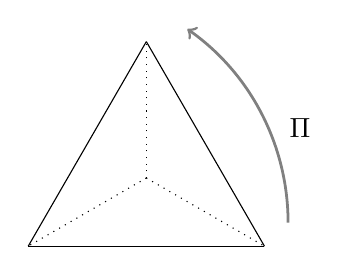
\begin{tikzpicture}[scale=3] \draw (0,0) --
        (1,0); \draw (0,0) -- (1/2,{sqrt(3)/2}); \draw (1/2,{sqrt(3)/2}) --
        (1,0); \draw[dotted] (1/2,{sqrt(3)/6}) -- (1/2,{sqrt(3)/2});
        \draw[dotted] (1/2,{sqrt(3)/6}) -- (0,0); \draw[dotted]
        (1/2,{sqrt(3)/6}) -- (1,0); \node at (1.15,0.5) {$\Pi$}; \draw [line
        width = 1, ->, gray] (1.1,0.1) arc [radius=1, start angle=0, end angle=
        55]; \end{tikzpicture} \label{fig:lookingdown} \end{figure}


    We have rotations $\Pi, \Pi^2$. There are 4 choices from the ``top''
    vertex, so 8 rotations of order 3.

    \underline{View looking down from the perspective on an edge.}
    \begin{figure}[h] \centering 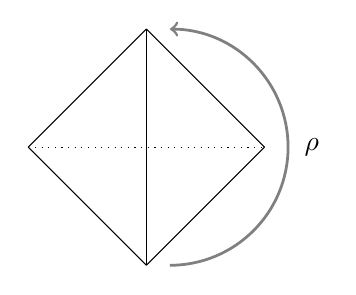
\begin{tikzpicture}[scale=3] \draw (0,0.5) --
        (0.5,1); \draw (1,0.5) -- (0.5,1); \draw (0,0.5) -- (0.5,0); \draw
        (1,0.5) -- (0.5,0); \draw (0.5,1) -- (0.5,0); \draw[dotted] (0,0.5) --
        (1,0.5); \node at (1.2,0.5) {$\rho$}; \draw [line width = 1, ->, gray]
        (0.6,0) arc [radius=0.5, start angle=-90, end angle=90];
      \end{tikzpicture} \label{fig:lookingdownedge} \end{figure}

    Rotation $\rho$ of order 2, one for each pair of opposite edges. So
    elements of order 2.

    The identity rotation makes up the total of 12.  \end{exmp}

  We found 12 rotations of a tetrahedron. Identity rotation and 8 rotations of
  order 3 (2 for each face), and 3 rotations of order 2.

  \textbf{Claim:} The rotations form an group isomorphic to $A_4$.

  \begin{proof} Number the vertices of the tetrahedron $1,2,3,4$. Identify each
    rotation with its effect on the vertex numbers.

    % figure
    \begin{figure}[!tbp] \centering \begin{minipage}[b]{0.4\textwidth}
        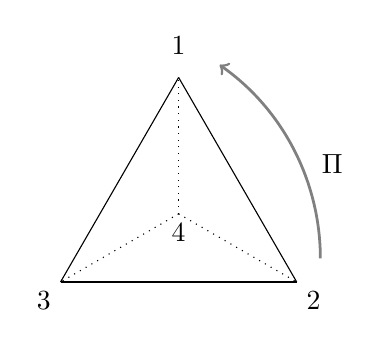
\begin{tikzpicture}[scale=3] \draw (0,0) -- (1,0); \node[below left] at
          (0,0) {3}; \node[below right] at (1,0) {2}; \node at (0.5,1) {1};
          \node[below] at (1/2,{sqrt(3)/6}) {4}; \draw (0,0) --
          (1/2,{sqrt(3)/2}); \draw (1/2,{sqrt(3)/2}) -- (1,0); \draw[dotted]
          (1/2,{sqrt(3)/6}) -- (1/2,{sqrt(3)/2}); \draw[dotted]
          (1/2,{sqrt(3)/6}) -- (0,0); \draw[dotted] (1/2,{sqrt(3)/6}) -- (1,0);
          \node at (1.15,0.5) {$\Pi$}; \draw [line width = 1, ->, gray]
          (1.1,0.1) arc [radius=1, start angle=0, end angle= 55];
        \end{tikzpicture} \end{minipage} \hfill
      \begin{minipage}[b]{0.4\textwidth} \begin{tikzpicture}[scale=3] \draw
          (0,0) -- (1,0); \node[below left] at (0,0) {1}; \node[below right] at
          (1,0) {3}; \node at (0.5,1) {2}; \node[below] at (1/2,{sqrt(3)/6})
          {4}; \draw (0,0) -- (1/2,{sqrt(3)/2}); \draw (1/2,{sqrt(3)/2}) --
          (1,0); \draw[dotted] (1/2,{sqrt(3)/6}) -- (1/2,{sqrt(3)/2});
          \draw[dotted] (1/2,{sqrt(3)/6}) -- (0,0); \draw[dotted]
          (1/2,{sqrt(3)/6}) -- (1,0); \end{tikzpicture} \end{minipage}
      \label{fig:pftriangle} \caption{This rotation corresponds to the
      permutation $(123).$} \end{figure} \begin{figure}[!tbp] \centering
      \begin{minipage}[b]{0.4\textwidth} 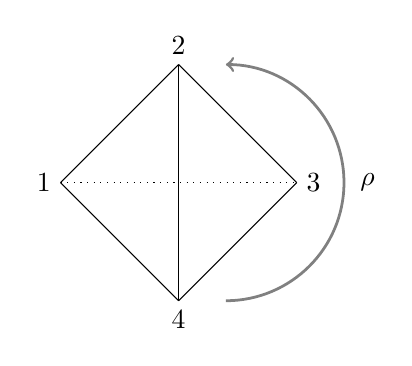
\begin{tikzpicture}[scale=3] \draw
          (0,0.5) -- (0.5,1); \node[left] at (0,0.5) {1}; \node[right] at
          (1,0.5) {3}; \node[above] at (0.5,1) {2}; \node[below] at (0.5,0)
          {4}; \draw (1,0.5) -- (0.5,1); \draw (0,0.5) -- (0.5,0); \draw
          (1,0.5) -- (0.5,0); \draw (0.5,1) -- (0.5,0); \draw[dotted] (0,0.5)
          -- (1,0.5); \node at (1.3,0.5) {$\rho$}; \draw [line width = 1, ->,
          gray] (0.7,0) arc [radius=0.5, start angle=-90, end angle=90];
        \end{tikzpicture} \end{minipage} \hfill
      \begin{minipage}[b]{0.4\textwidth} \label{fig:lookingdownedge} \centering
        \begin{tikzpicture}[scale=3] \node[left] at (0,0.5) {3}; \node[right]
          at (1,0.5) {1}; \node[above] at (0.5,1) {4}; \node[below] at (0.5,0)
          {2}; \draw (0,0.5) -- (0.5,1); \draw (1,0.5) -- (0.5,1); \draw
          (0,0.5) -- (0.5,0); \draw (1,0.5) -- (0.5,0); \draw (0.5,1) --
          (0.5,0); \draw[dotted] (0,0.5) -- (1,0.5); \end{tikzpicture}
      \end{minipage} \label{fig:lookingdownedge} \caption{This rotation
      corresponds to the permutation $(13)(24)$.} \end{figure} Easy to check
    that this gives a bijection between the set of rotations and $A_4$, since
    every rotation is giving an even permutation, and $|A_4|=12$.  Now
    composing rotations is equivalent to composing permutations, so the
    bijection respects multiplication. So the rotations form a group isomorphic
    to $A_4$.  \end{proof}

  There are other symmetries of the tetrahedron, namely reflections.

  Take a plane passing through two vertices, and the midpoint of the edge
  opposite the edge through these two vertices. A reflection through this plane
  is a symmetry of the tetrahedron. 

  Let this reflection be $g$. Let $R$ be the group of rotations. Then $g
  \not\in R$, and so $gR \neq R$. So $G \supseteq R \cup gR$ (where $G$ is the
  symmetry group of the tetrahedron). 

  So $|G| \geq 24$.

  But any symmetry must fix the set of vertices (as a set), and symmetry is
  determined by how it permutes the vertices.

  Since there are only 24 permutations of the vertices, we have $|G|=24$, and
  $G \ism S_4$.  \newpage \subsection{Counting Using Groups} Given an equilateral
  triangle, how many different ways are there of colouring the edges red or
  green? (where colourings which are the same up to rotation or reflection
  count as the same). 

  Possibilities: \begin{itemize} \item All edges red \item Two edges red, one
      green \item One red, two green \item All green \end{itemize} How about a
    more complicated example - say 10 colours available instead of 2. We need a
    technique.

 Idea is: \begin{itemize} \item $\Gamma$ a structure (i.e. a
     triangle/polygon/subset of $\reals^n$).  \item $H$ a group of symmetries
     of $\Gamma$. (Maybe $H$ is not the whole symmetry group.) \item $C$ a set
       of colours.  \end{itemize}

 Apply colours from $C$ to points/lines of $\Gamma$.

 If two colourings $A,B$ satisfy $A=hB$ for some $h \in H$, treat $A$ and $B$
 as the same. Count the total number of colourings.\\

 \begin{definition} If $A$ is a colouring of $\Gamma$, then the set $\left\{ hA
   : h \in H \right\}$ is the \emph{orbit} of $A$ under the action of $H$.\\

   \begin{exmp} $\Gamma$ is an equilateral triangle, $C = \left\{ red, green
     \right\}$, colouring the edges, $H=$ symmetry group $=D_6$.

     $A =$ \begin{figure}[h] \centering 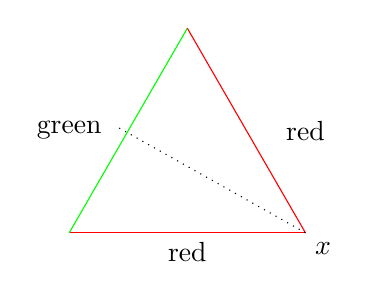
\begin{tikzpicture}[scale=3] \node at
         (0,{sqrt(3)/4}) {green}; \node at (1,{sqrt(3)/4}) {red}; \node[below]
         at (0.5,0) {red}; \draw[red] (0,0) -- (1,0); \draw[green] (0,0) --
         (1/2,{sqrt(3)/2}); \draw[red] (1/2,{sqrt(3)/2}) -- (1,0);
         \draw[dotted] (1,0) -- (0.2, 0.45);
         \node[below right] at (1,0) {$x$};
       \end{tikzpicture} \label{fig:lookingdown} \end{figure}

     Orbit of $A = $ \begin{figure}[h] \centering
       \begin{tikzpicture}[scale=2.5] \node at (0,{sqrt(3)/4}) {$g$}; \node at
         (1,{sqrt(3)/4}) {$r$}; \node[below] at (0.5,0) {$r$}; \draw[red] (0,0) --
         (1,0); \draw[green] (0,0) -- (1/2,{sqrt(3)/2}); \draw[red]
         (1/2,{sqrt(3)/2}) -- (1,0); \end{tikzpicture}\hfill
       \begin{tikzpicture}[scale=2.5] \node at (0,{sqrt(3)/4}) {$r$}; \node at
         (1,{sqrt(3)/4}) {$g$}; \node[below] at (0.5,0) {$r$}; \draw[red] (0,0) --
         (1,0); \draw[red] (0,0) -- (1/2,{sqrt(3)/2}); \draw[green]
         (1/2,{sqrt(3)/2}) -- (1,0); \end{tikzpicture}\hfill
       \begin{tikzpicture}[scale=2.5] \node at (0,{sqrt(3)/4}) {$r$}; \node at
         (1,{sqrt(3)/4}) {$r$}; \node[below] at (0.5,0) {$g$}; \draw[green] (0,0)
         -- (1,0); \draw[red] (0,0) -- (1/2,{sqrt(3)/2}); \draw[red]
         (1/2,{sqrt(3)/2}) -- (1,0); \end{tikzpicture} \end{figure}


   \end{exmp} \end{definition} \begin{definition} If $A$ is a colouring of
   $\Gamma$, then the set $\left\{ h \in H : hA=A \right\}$ is the
   \emph{stabiliser} of $A$ in $H$.

   The stabiliser of $A$ is a subgroup of $H$. (Exercise.)\\

   \begin{exmp} $\Gamma, H, A$ as in the examples above.

     Stabiliser of $A$ in $H$ is $\left\{ id,t \right\}$, where $t$ is the
     reflection through the axis $x$.\\ \end{exmp} \end{definition}

 \begin{theorem} Assuming that the group $H$ is finite, we have \[
   \big|\text{Orbit of }A\big| \big|\text{Stabiliser of } A\big|=\big|H\big| \]
   for all colourings $A$.
  
   \label{thm:orbitstabiliser} \end{theorem}

 Recall: We have a structure $S$ (e.g. edges of a polygon, vertices of a
 polygon, etc.) $G$ The symmetry group. $C$ a set of colours. \emph{How many
 colourings of $S$ are possible, if we don't distinguish colourings related by
 a symmetry?}

 Let $\mathcal{A}=$ set of all possible colourings. For $A \in \mathcal{A}$, we
 defined Orbit: $\Orb_G(A)=\left\{ gA : g \in G \right\}$ and Stabiliser:
 $\Stab_G(A) = \left\{ g \in G : gA = A \right\}$ and Orbit-Stabiliser Theorem
 says $|\Orb_G(A)||\Stab_G(A)|=|G|$.

 \begin{proof} (Idea): Suppose $g_1,g_2\in G$ are such that $g_1A=g_2A$. Then
   $g_2^{-1}g_1A=A$, and so $g_2^{-1}g_1A \in \Stab_G(A)$. So
   $g_1\Stab_G(A)=g_2\Stab_G(A)$. Conversely, if $g_1\Stab_G(A)=g_2\Stab_G(A)$
   then $g_1A=g_2A$. So elements of $\Orb_G(A)$ are in bijection with the
   cosets of $\Stab_G(A)$ in $G$. Since the number of cosets is
   $|G|/|\Stab_G(A)|$, we're done.  \end{proof} 

 \begin{exmp} Take $S=$ edges of a square and $G=D_8$ (full symmetry group). $C
   = \left\{ red, green \right\}=\left\{ r,g \right\}$. 
   
   So $A=$ \begin{figure}[h] \centering \begin{tikzpicture}[scale=2]
       \draw[red] (0,0) -- (0,1); \draw[green] (0,0) -- (1,0); \draw[green]
       (1,0) -- (1,1); \draw[red] (0,1) -- (1,1); \draw[dotted] (0,1) -- (1,0);
       \node[below right] at (1,0) {$x$}; \node[below] at (0.5,0) {$g$};
       \node[left] at (0,0.5) {$r$}; \node[right] at (1,0.5) {$g$};
       \node[above] at (0.5,1) {$r$}; \end{tikzpicture}
     \label{fig:coloursquare} \end{figure}
 
 \end{exmp}

  Then orbit is the rotations:

  $\Orb_G(A)=$ \begin{figure}[h] \centering 
    \begin{tikzpicture} 
      \draw[red] (0,0) -- (0,1); 
      \draw[green] (0,0) -- (1,0); 
      \draw[green] (1,0) -- (1,1);
      \draw[red] (0,1) -- (1,1); 
      \node[below] at (0.5,0) {$g$}; 
      \node[left] at  (0,0.5) {$r$}; 
      \node[right] at (1,0.5) {$g$}; 
      \node[above] at (0.5,1) {$r$}; 
    \end{tikzpicture}\hfill 
    \begin{tikzpicture} 
      \draw[green] (0,0) --  (0,1); 
      \draw[green] (0,0) -- (1,0); 
      \draw[red] (1,0) -- (1,1);
      \draw[red] (0,1) -- (1,1); 
      \node[below] at (0.5,0) {$g$}; \node[left]
      at (0,0.5) {$g$}; \node[right] at (1,0.5) {$r$}; \node[above] at (0.5,1)
      {$r$}; 
    \end{tikzpicture}\hfill 
    \begin{tikzpicture} 
      \draw[green] (0,0) --  (0,1); 
      \draw[red] (0,0) -- (1,0); 
      \draw[red] (1,0) -- (1,1);
      \draw[green] (0,1) -- (1,1); 
      \node[below] at (0.5,0) {$r$}; 
      \node[left] at (0,0.5) {$g$}; 
      \node[right] at (1,0.5) {$r$}; 
      \node[above] at (0.5,1) {$g$}; 
    \end{tikzpicture}\hfill 
    \begin{tikzpicture} 
      \draw[red] (0,0) --  (0,1); 
      \draw[red] (0,0) -- (1,0); 
      \draw[green] (1,0) -- (1,1);
      \draw[green] (0,1) -- (1,1); 
      \node[below] at (0.5,0) {$r$}; 
      \node[left] at (0,0.5) {$r$}; 
      \node[right] at (1,0.5) {$g$}; 
      \node[above] at (0.5,1) {$g$}; 
    \end{tikzpicture} \label{fig:coloursquaremult} 
  \end{figure}

   $\Stab_G(A)=\left\{ id, \text{ reflection through }x \right\}$.

   And we have $|\Orb_G(A)||\Stab_G(A)|=4 \times 2 = 8 = |G|$.\\ \begin{lemma}
     (Orbit-Counting, Burnside). The number of orbits of $G$ on colourings is
     \[ \frac{1}{G} \sum_{g \in G}\fix(g) \] Where $\fix(g)$ is the number of
     colourings fixed by $g$.  \label{lem:orbitcounting} \end{lemma}

   \begin{proof} Notice that \begin{align*} \sum_g \fix(g) &= \sum_g |\left\{ A
       : gA = A \right\}| \\ &= |\left\{ (g,A) : g \in G, A \in
         \mathcal{A},gA=A \right\}|\\ &= \sum_{A \in \mathcal{A}}|\left\{ g \in
         G | gA = A \right\}|\\ &= \sum_{A \in \A} |\Stab_G(A)|\\ &= \sum_{A
         \in \A} \frac{|G|}{|\Orb_G(A)|} \end{align*}

so

\begin{align*} \frac{1}{|G|}\sum_{g \in G} \fix(g) = \sum_{A \in \A}
  \frac{1}{\Orb_G(A)}.  \end{align*} But every orbit counts exactly 1 in this
sum since the orbit $O$ has $|O|$ colourings, each counting $\frac{1}{|O|}$. So
$\sum_{A \in \mathcal{A}}\frac{1}{|\Orb_G(A)|}$ is the number of orbits.
\end{proof}

\begin{exmps} A necklace has 6 beads, each red or green. How many different
  necklaces are possible?

  Model the necklace as vertices of a regular hexagon.

  The appropriate symmetry group is $D_{12}$ (full symmetry group). Consider the
  symmetries as permuations of the beads.

  \begin{itemize} \item Rotations: \begin{itemize} \item $id$ fixes all $2^6$
          colourings.  \item $R_\pi = (14)(25)(36)$.  We need $1,4$ the same
          colour etc.  \item $R_\pi$ has 3 cycles, so $2^3$ colourings are
            fixed.

      \item $R_{2\pi/3},R_{4\pi/3}=(135)(246),(153)(264)$.  Both have 2 cycles,
      so fix $2^2$ colourings.  \item $R_{2\pi/6},R_{10\pi/6}=(123456)(165432)$

       Just one cycle, so fix 2 colourings.  \end{itemize}
      

     \item Reflections: Axis through opposite edges (3 reflections)
       $(12)(36)(45)$. 
% fig
       \begin{figure}[h] \centering 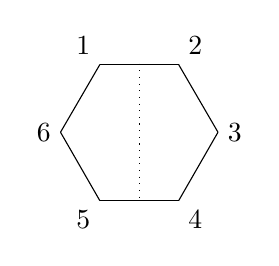
\begin{tikzpicture} 
           \draw[dotted] (1,1.74) -- (1,0); 
           \draw (0,0.87) -- (0.5,0); 
           \node[left] at (0,0.87) {6};
           \draw (0.5,0) -- (1.5,0); 
           \node[below left] at (0.5, 0) {5};
           \draw (1.5,0) -- (2,0.87); 
           \node[below right] at (1.5, 0) {4};
           \draw (2,0.87) -- (1.5,1.73); 
           \node[right] at (2,0.87) {3};
           \draw (1.5,1.73) -- (0.5,1.73); 
           \node[above right] at (1.5, 1.73) {2};
           \draw (0.5,1.73) -- (0,0.87); 
           \node[above left] at (0.5,1.73) {1};
         \end{tikzpicture}

         \label{fig:necklace1} \end{figure}
      
       
       3 cycles, so $2^3$ fixed colourings. 
% fig
Axis through opposite vertices (3 reflections) $(13)(2)(46)(5)$.

       \begin{figure}[h] 
         \centering 
         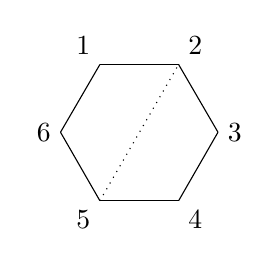
\begin{tikzpicture} 
           \draw[dotted] (0.5,0) -- (1.5,1.73); 
           \draw (0,0.87) -- (0.5,0); 
           \node[left] at (0,0.87) {6};
           \draw (0.5,0) -- (1.5,0); 
           \node[below left] at (0.5, 0) {5};
           \draw (1.5,0) -- (2,0.87); 
           \node[below right] at (1.5, 0) {4};
           \draw (2,0.87) -- (1.5,1.73); 
           \node[right] at (2,0.87) {3};
           \draw (1.5,1.73) -- (0.5,1.73); 
           \node[above right] at (1.5, 1.73) {2};
           \draw (0.5,1.73) -- (0,0.87); 
           \node[above left] at (0.5,1.73) {1};
         \end{tikzpicture}

         \label{fig:necklace1} \end{figure}
       

       4 cycles. so $2^4$ fixed colourings.

       
       Now the Orbit-Counting lemma gives

       \begin{align*} \# \text{orbits} &= \frac{1}{12}(64 + 8 + 2\times4 +
         2\times 2 + 3 \times 8 + 3 \times 16)\\ &= \frac{1}{12}\times 156 \\
         &= 13.  \end{align*} \end{itemize} \end{exmps}

\section{Linear Algebra} \subsection{Determinants} We know determinants for $2
\times 2$ matrices: \[ \begin{vmatrix} a & b \\ c & d \end{vmatrix} = ad - bc
\] And $3 \times 3$ matrices: \[ \begin{vmatrix} a & b & c \\ d & e & f \\ g &
    h & i \end{vmatrix} = a \begin{vmatrix} e & f \\ h & i \end{vmatrix} -
b\begin{vmatrix} d & f \\ g & i \end{vmatrix} + c\begin{vmatrix} d & e \\ g & h
\end{vmatrix} = aei - afh - bdi +bfg +cdh-ceg.  \]

Let $A=(a_{ij})$  be an $n \times n$ matrix.

Write $A_{ij}$ for the minor obtained by deleting the $i^{th}$ row and the
$j^{th}$ column. We could define $\det A$ (or $|A|$ ) by analongy with the $3
\times 3$ case, as

\[ |A| = a_{11}|A_{11}| - a_{12}|A_{12}| + a_{13}|A_{13}| \cdots +
(-1)^{n-1}a_{1n}|A_{1n}|.  \]

(Definition by expansion along the first row.)

This is a \emph{recursive} definition -- $n \times n$ determinants are defined
in terms of $(n-1) \times (n-1)$ determinants.

Expanding along a different row (or a column) would give the same result (proof
later)


In fact we will use an alternative definition.

The terms in \[ \begin{vmatrix} a & b & c \\ d & e & f \\ g & h & i
\end{vmatrix} \]

are each a product of three entries, one from each row and column.

Suppise we pick the entry in column $f(i)$ from row $i$, then $f$ is a
permutation of $\left\{ 1,2,3 \right\}$. So the terms correspond to elements of
$S_3$.

\begin{align*} aei &\leftrightarrow \text{id} \\ bfg &\leftrightarrow (123) \\
  cdh &\leftrightarrow (132) \\ -bdi &\leftrightarrow (12) \\ -ceg
  &\leftrightarrow (13) \\ -afh &\leftrightarrow (23).  \end{align*} Notice the
sign before each term is just the signature of the corresponding permutation.

Similarly for the $2 \times 2$ determinant: $\begin{vmatrix}a & b \\ c &
  d\end{vmatrix}$

\begin{align*} ad &\leftrightarrow \text{id} \\ -bc &\leftrightarrow (12).
\end{align*}

\begin{definition} Let $A$ be an $n \times n$ matrix, $A = (a_{ij})$. The
  determinant of $A$ is \[ \det A = \sum_{\sigma \in S_n} \sgn(\sigma)
  a_{1\sigma(1)}a_{2\sigma (2)}\dots a_{n \sigma (n)}.  \] \end{definition}

\begin{proposition} \label{prp:swaprows} Suppose that $B$ is obtained from $A$
  by swapping two rows. Then I claim $\det B = -\det A$.  \end{proposition}

  \begin{proof} Suppose that rows $p$ and $q$ are the rows that are going to be
    swapped. Let $A=(a_{ij}),B=(b_{ij})$. I claim that we can write \[ b_{ij} =
    a_{\tau (i) j}, \quad\text{where }\tau = (pq) \quad (2-\text{cycle}).\]

      \begin{align*} \det B &= \sum_{\sigma \in S_n} \sgn(\sigma)
        b_{1\sigma(1)}b_{2\sigma (2)}\dots b_{n \sigma (n)}\\ &= \sum_{\sigma
        \in S_n} \sgn(\sigma) a_{\tau(1)\sigma(1)}a_{\tau(2)\sigma (2)}\dots
        a_{\tau(n) \sigma (n)}\\ &= \sum_{\sigma \in S_n} \sgn(\sigma)
        a_{1\tau^{-1}\sigma(1)}a_{2\tau^{-2}\sigma (2)}\dots a_{n\tau^{-n}
      \sigma (n)} \end{align*} (Same $n$ factors in each product, but in a
    different order). Notice that $\tau = \tau^{-1}$.  \begin{align*} &=
      \sgn{\tau} \sum_{\sigma \in
      S_n}\sgn(\tau)\sgn(\sigma)a_{1\tau\sigma(1)}\dots a_{n \tau\sigma(n)} \\
      &= - \sum_{\sigma \in S_n}\sgn(\tau\sigma)a_{1\tau\sigma(1)}\dots a_{n
      \tau\sigma(n)} \\ &= - \sum_{\tau\sigma \in
      S_n}\sgn(\tau\sigma)a_{1\tau\sigma(1)}\dots a_{n \tau\sigma(n)}
    \end{align*} Since the sum is over all group elements in either case.
    \begin{align*} &= -\det A.  \end{align*} \end{proof}

  \begin{proposition}\hfill \label{prp:rowssame} \begin{enumerate}[(i)] \item If $A$
          has an all-0 row, then $\det A=0$.  \item If $A$ has two rows the
          same then $\det A=0$.  \item If $A$ is triangular (upper or lower)
            then $\det A=a_{11}a_{22}\dots a_{nn}$ \end{enumerate}


  \end{proposition}

  \begin{proof}\hfill 
    \begin{enumerate}[(i)]
      \item 
    Suppose that $A$ has all $0$s in row $i$. Then
    $a_{i\sigma(i)}=0$ for all $\sigma \in S_{n}$. So $a_{1\sigma(1)}\dots
    a_{n\sigma(n)}=0$, for all $\sigma$.
    So $\det A = 0$.
  \item
    Suppose that $A$ has rows $p$ and $q$ the same. Let $B$ be the matrix
    obtained from $A$ by exchanging rows $p$ and $q$. Then $\det B=-\det A$ by
    Prop \ref{prp:swaprows}.  But clearly $B=A$, so $\det A = - \det A$. So
    $\det A=0$.
  \item
    Let $\sigma$ be a non-identity permutation in $S_n$. There must exist $i,j
    \in \left\{ 1,\dots n \right\}$ with $\sigma(i) > i, \sigma(j)<j$. Whether
    $A$ is upper-or-lower-triangular, one of $a_{i\sigma(i)}$ or
    $a_{j\sigma(j)}$ is 0. So $a_{1\sigma(1)}\dots a_{n\sigma(n)}=0$, and so
    the only $\sigma \in S_n$ which contributes to the $\det A$ is the
    identity.

    Hence $\det A = \sgn(\id)a_{11}\dots a_{nn}$ and $\sgn(\id)=+1$, giving the
    result. 

    \end{enumerate}


  \end{proof} \begin{proposition} (Row operations).  \begin{enumerate}[(i)] \item
          Let $B$ be obtained by swapping two rows. Then $\det B=-\det A$.
        \item Let $B$ be obtained from $A$ by multiplying a row by a scalar
          $\lambda$.

          Then $\det B = \lambda \det A$.  \item Let $B$ be obtained from $A$
            by adding $\lambda$ times row $i$ to row $j$, where $i \neq j$.
            Then $\det B = \det A$.  \end{enumerate} \end{proposition}
    \begin{proof}\hfill \begin{enumerate}[(i)] \item  Suppose that $A$ has all
            0s in row $i$. Then $a_{i\sigma(i)} = 0$ for all $\sigma \in n$.
          So $a_{1\sigma(1)}\dots a_{n\sigma(n)} = 0$, for all $\sigma$. So
        $\det A = 0$.  \item  Suppose that $A$ has rows $p$ and $q$ the same.
          Let $B$ be the matrix obtained from $A$ by exchanging rows $p$ and
          $q$. Then $\det B = -\det A $ (Proposition \ref{prp:swaprows}.) But
          clearly $B = A$, so $\det A = -\det A$. So $\det A = 0$.

     \item Let $\sigma$  be a non-identity permutation. There must exist $i, j
       \in \left\{ 1,\dots ,n \right\}$ with $\sigma(i) > i$ and $\sigma(j) <
       j$. Whether $A$ is upper or lower triangular, one of $a_{i\sigma(i)}$ or
       $a_{j\sigma(j)}$ is 0. So $a_{1\sigma(1)}\dots a_{n\sigma(n)} = 0$, for
       all non-identity $\sigma$’s, and so the only $\sigma \in S_n$ which
       contributes to $\det A$ is the identity. Hence $\det A = \sgn(\id)
       a_{11}\dots a_{nn}$. And $\sgn(\id) = +1$, giving the result.
   \end{enumerate} \end{proof}

\begin{proposition}\hfill \label{prp:rowops} \begin{enumerate}[(i)] \item Let $B$ be
        obtained from $A$ by swapping two rows. Then $\det B = - \det A$.
      \item Let $B$ be obtained from $A$ by multiplying a row by a scalar
        $\lambda$. Then $\det B = \lambda\det A$.  \item Let $B$ be obtained
          from $A$ by adding $\lambda$ times row $i$ to row $j$ $(i \neq j)$.
          Then $\det B = \det A$.  \end{enumerate} \end{proposition}

\begin{proof}\hfill \begin{enumerate}[(i)] \item This is Proposition
        \ref{prp:swaprows}.  \item Suppose we multiply row $p$ by scalar
          $\lambda$. So \[ b_{ij} = \begin{cases} \lambda a_{ij}, & \text{if }
              i=p \\ a_{ij}, & \text{otherwise} \end{cases} \] For $\sigma \in
            S_n$ we have \begin{align*} b_{1\sigma(1)}\dots b_{n\sigma(n)} &=
              a_{1\sigma(1)}\dots \lambda a_{p\sigma(p)}\dots a_{n \sigma(n)}
              \\ &= \lambda (  a_{1\sigma(1)}\dots  a_{n\sigma(n)} )
            \end{align*} So \begin{align*} \sum_\sigma \sgn (\sigma)
              b_{1\sigma(1)}\dots b_{n\sigma(n)} &= \lambda \sum_\sigma
              \sgn(\sigma)  a_{1\sigma(1)}\dots a_{n\sigma(n)}\\ \implies \det
              B &= \lambda \det A \end{align*} \item We have $b_{ij} = a_{jk} +
              \lambda_{ik}$ for all $k$ Also, $b_{kk}=a_{kk}$ is $k \neq j$. We
              have, for $\sigma \in S_n$,

      \begin{align*} b_{1\sigma(1)}\dotsb_{n\sigma(n)} &= a_{1 \sigma(1)} \dots
        ( a_{j \sigma(j)} + \lambda  a_{i \sigma(j)} ) \dots a_{n\sigma(n)} \\
        &= \elemt{a}{1} \dots \elemt{a}{j} \dots\elemt{a}{n} + \elemt{a}{1}
        \dots \lambda a_{i\sigma(j)} \dots a_{n\sigma(n)} \end{align*} It
      follows that

      \[ |B| = |A| + \lambda \begin{vmatrix} a_{11} & \cdots & a_{1n}\\ \vdots
          &        & \vdots \\ a_{i1} & \cdots & a_{in} \\ \vdots &        &
          \vdots \\ a_{i1} & \cdots & a_{in} \\ \vdots &        & \vdots \\
          a_{n1} & \cdots & a_{nn} \\ \end{vmatrix} \] And this is 0 since the
        matrix on the right has two rows the same (Prop. \ref{prp:rowssame}).
    \end{enumerate} \end{proof}

\begin{exmp} What is the determinant of \[ \left(\begin{matrix} 1 & 2 & 2 & 0
    \\ 1 & 4 & 0 & 3 \\ -1 & 0 & -2 & 3 \\ 1 & 0 & 8 & -6 \end{matrix}\right)
\] Use row operations. By Prop. \ref{prp:rowops} we have \begin{align*} |A| =
  \begin{vmatrix} 1 & 2 & 2 & 0 \\ 1 & 4 & 0 & 3 \\ -1 & 0 & -2 & 3 \\ 1 & 0 &
    8 & -6 \end{vmatrix} &= \begin{vmatrix} 1 & 2 & 2 & 0 \\ 0 & 2 & -2 & 3 \\
    0 & 0 & 2 & 0 \\ 0 & 0 & 4 & -3 \end{vmatrix}\\ &= \begin{vmatrix} 1 & 2 &
    2 & 0 \\ 0 & 2 & -2 & 3 \\ 0 & 0 & 2 & 0 \\ 0 & 0 & 0 & -3 \end{vmatrix}\\
  &= -12 \end{align*}

\end{exmp}

\begin{proposition}
  \label{prp:detab} Suppose that $B$ can be obtained from $A$ by row
operations: \begin{enumerate}[(i)] \item Exchanging rows \item Scaling rows by
    non-zero scalar \item Adding multiples of one-row to another row.
  \end{enumerate} Then $\det B = 0 \iff \det A = 0$.  \end{proposition}

\begin{proof} Clear from Prop. \ref{prp:rowops}.  \end{proof}

\begin{proposition} \label{prp:dettran} Let $A$ be an $n\times n$ matrix. Then
  $|A| = |A|^T$  (where $A^T$ is the \emph{transpose} of $A$.)
\end{proposition}

\begin{proof} Let $A^T = (b_{ij})$. Then $b_{ij} = a_{ji}$. Let $\sigma \in
  S_n$. We have \begin{align*} \elemt{b}{1} \dots \elemt{b}{n} &=
    a_{\sigma(1)1} \dots a_{\sigma(n)n} \\ &= a_{1\sigma^{-1}(1)}\dots a_{n
      \sigma^{-1}(n)} \end{align*}

So 

\[ \det A^T = \sum_{\sigma \in S_n}\sgn(\sigma)  a_{1\sigma^{-1}(1)}\dots a_{n
\sigma^{-1}(n)} \] Now summing over all $\sigma$ is equivalent to summing over
$\sigma^{-1}$ and $\sgn(\sigma) = \sgn(\sigma^{-1})$

\begin{align*} &= \sum_{\sigma^{-1} \in S_n}\sgn
  (\sigma^{-1})a_{1\sigma^{-1}(1)}\dots a_{n \sigma^{-1}(n)}\\ &= \det A
\end{align*} \end{proof} Proposition \ref{prp:dettran}  implies that all of our
results concerning rows and row operations also hold for columns / column
operations (since columns of $A$ are the rows of $A^T$).

\subsection*{Expansion along rows / columns} Let $A = (a_{ij} )$, and let
$A_{ij}$ be the minor obtained by deleting row $i$ and column $j$. Then

\textbf{Claim:} \[ \det A = \sum_{j=1}^n (-1)^{i+j}a_{ij}|A_{ij}|, \quad
\text{for any } i \]

\begin{proof} First suppose $i = 1$. We have from the definition that $|A|$ is
  a sum over all elements $\sigma \in S_n$. Consider all $\sigma$ such that
  $\sigma(1) = 1$. It's not hard to see that

  \[ \sum_{\sigma(1)=1}\sgn(\sigma)a_{11}a_{2\sigma(1)}\dots a_{n\sigma(n)} =
  a_{11}|A_{11}| \]

  How about $\sigma$ such that $\sigma(1) = 2$? Let $B$ be obtained from $A$ by
  swapping columns 1 and 2. Then \[ B = \begin{vmatrix} a_{12} & a_{11} &
      \cdots & a_{1n} \\ a_{22} & a_{21} & \cdots & a_{2n} \\ \vdots & \vdots &
      & \vdots  \\ a_{n2} & a_{n1} & \cdots & a_{nn} \end{vmatrix} \] So terms
    of $\det A$ corresponding to $\sigma(1) = 2$ are the same as the terms of
    $b_{11}|B_{11}|$. But swapping two columns negates the determinant, so \[
      \sum_{\sigma(1)=2}\sgn (\sigma) a_{12}a_{2\sigma(2)} \dots a_{n\sigma(n)}
      = -b_{11}|B_{11}| = -a_{12}|A_{12}| \] \end{proof} 
    
    \[
    A = \left( 
    \begin{matrix}
      a_{11} & a_{12} & \dots & a_{1n} \\
      \vdots &        &       & \vdots \\
      a_{n1} & a_{n2} & \dots & a_{nn}
    \end{matrix}
    \right)
  \]
  \[
    B = \left( 
    \begin{matrix}
      a_{12} & a_{11} & \dots & a_{1n} \\
      \vdots &        &       & \vdots \\
      a_{n2} & a_{n1} & \dots & a_{nn}
    \end{matrix}
    \right)
    \]

   ($A$ with columns 1 and 2 swapped)

   We have $|B| = -|A|$ (Prop \ref{prp:swaprows}).

   If $\sgn(\sigma)a_{1\sigma(1)}\dots a_{n\sigma(n)}$ is a term of $|A|$, 
   then $-\sgn(\sigma)a_{1\sigma(1)}\dots a_{n\sigma(n)}$ 
   must be a term in $|B|$.

   We know that the terms of $|B|$ including $b_{11}=a_{12}$ are
   given by $b_{11}|B_{11}| = a_{12}|A_{12}|$.

   Hence the terms of $|A|$ including $a_{12}$ are given by  $-a_{12}|A_{12}|$.

   How about the terms of $|A|$ including $a_{13}$? 
   Bring the 3\ts{rd} columns to the front, without changing the order
   of the columns. Do this by first swapping columns 1 and 3, then 2 and 3.

   (Note $(123)=(23)(13)$.)
   
   If $B$ is the resulting matrix then 
   $|B|=|A|$ (Since we've swapped columns twice.)

   \[
   B = \left( 
   \begin{matrix}
     a_{13} & a_{11} & a_{12} & \dots & a_{1n} \\
     \vdots &        &        &       & \vdots \\
     a_{n3} & a_{n1} & a_{n2} & \dots & a_{nn}
   \end{matrix}
   \right)
   \]
  

   The  terms of $|B|$ including $a_{13}$ are given $a_{13}|A_{13}|$. So
   these are the terms of $|A|$ too.

   Continue in this way. Since bringing column $j$ to the front induces a $j-$
   cycle, we get $|B|=(-1)^{j+1}|A|$. So we end up with 
   \begin{align*}
     |A| &= a_{11}|A_{11}| - a_{12}|A_{12}| + a_{13}|A_{13}| - \dots\\
     &= \sum_{j=1}^n (-1)^{j+1}a_{ij}|A_{ij}|.
   \end{align*}
   This accounts for expansion along the $1^{st}$ row.

   How about expanding along row $i$?

   We can do this by first bringing row $i$ to the top without changing the
   order of the other rows.

   This induces an $i-$cycle on the rows, which can be done by swapping
   rows $i-1$ times.

   So if $B$ is the resulting matrix, then $|B|=(-1)^{i-1}|A|$.

   So we get

   \begin{align*}
     |A| &= (-1)^{i-1} \sum_{j=1}^n (-1)^{j+1} a_{ij} |A_{ij}| \\
     &= \sum_{j=1}^n (-1)^{i+j} a_{ij} |A_{ij}|.
   \end{align*}

   \begin{remark}
     We can also find determinants by expansion along columns. (By Prop.
     \ref{prp:dettran}).\\
   \end{remark}
  
   \begin{proposition}
     Let $A$ be an $n\times n$ matrix.
     The following statements are equivalent. 
     \begin{enumerate}[(i)]
       \item $|A| \neq 0$.
       \item $A$ is invertible.
       \item The system of equations $A\underline{x}=\underline{0}$ has no 
         solutions except $\underline{x}=\underline{0}$.
       \item $A$ can be reduced to $I$ by row operations.
     \end{enumerate}
   \end{proposition}

   \begin{proof}
     $(2) \iff (3) \iff (4)$ from $M1GLA$.
     \begin{itemize}
       \item[$(4) \iff (1)$] Suppose $I$ can be obtained from $A$. by row
         operations. We know $|I|\neq 0$ and so $|A|\neq 0$, by Prop.
         \ref{prp:detab}.

       \item[$(1)\iff (4)$] Let $A_{ech}$ be the row echelon form of $A$.
         Then $A_{ech}$ is obtained from $A$ by row operations.

         So if $|A|\neq 0$ then $|A_{ech}| \neq 0$.

         So $A_{ech}$ has no all$-0$ rows.

         Hence $A_{ech}$ can be transferred to $I$ by row operations.
     \end{itemize}
   \end{proof}

   The last major property of determinants that we want is $\Det{AB} =
   \Det{A}\Det{B}$. For this we require:

   \subsubsection*{Elementary Matrices}

   \[
     A_{i}(\lambda) = \left( 
     \begin{matrix}
       1 &        & & & & \\
         & \ddots & & & & \\
         &        & 1 & & & \\
         &        &   & \lambda & & \\
         &        &   &         & \ddots & \\
         &        &   &         &        & 1 \\
     \end{matrix}
     \right)
   \]
   $\lambda \neq 0$, $I$ with row $i$ scaled by $\lambda$.

  \[
    B_{ij} = \left( 
    \begin{matrix}
     1 &  & & & & &  \\
      & \ddots & & & & & \\
      & & 0 & & 1 & &  \\
      & & &  \ddots & &  & &  \\
      & & 1 & & 0 & &  \\
      &  & & & & \ddots & \\
      &  & & & & &1  \\
    \end{matrix}
    \right)
  \]
  $i \neq$ j, $I$ with rows $i$ and $j$ swapped.

  \[
    C_{ij}(\lambda) = \left( 
    \begin{matrix}
      1 &        &         &  \\
        & \ddots & \lambda &  \\
        &        &         & 1
    \end{matrix}
    \right)
  \]

    $i \neq j$, $\lambda \neq 0$. $I$ with $\lambda$ times row $j$ added to 
    row $i$.

    The elementary matrices correspond to elementary row operations.

    If $M$ is an $n \times n$ matrix with rows $r_1,\dots r_n$ then:
   
    \begin{itemize}
      \item 
    Multiplying row $r_i$ by $\lambda$ $\longrightarrow$ $A_i(\lambda)M$
    \item
    Swapping rows $r_i$ and $r_j$ $\longrightarrow$ $B_{ij}M$
    \item
    Adding $\lambda r_j$ to $r_i$ $\longrightarrow$ $C_{ij}(\lambda)M$.\\
    \end{itemize}
    \begin{exmps}
  $A_2(3) = \left( 
\begin{matrix}
  1 & 0 \\
  0 & 3
\end{matrix}
  \right)$.

  \begin{align*}
  \left( 
  \begin{matrix}
    1 & 0 \\
    0 & 3
  \end{matrix}
  \right)\left( 
  \begin{matrix}
    p & q \\
    r & s
  \end{matrix}
  \right) = \left( 
  \begin{matrix}
    p & q \\
    3r & 3s
  \end{matrix}
  \right)
\end{align*}

  For $
    B_{12} = \left( 
  \begin{matrix}
    0 & 1 \\
    1 & 0
  \end{matrix}
  \right)
$

\begin{align*}  
\left( 
  \begin{matrix}
    0 & 1\\
    1 & 0
  \end{matrix}
  \right)\left( 
  \begin{matrix}
    p & q \\
    r & s
  \end{matrix}
  \right) = \left( 
  \begin{matrix}
    r & s \\
    p & q
  \end{matrix}
  \right)
\end{align*}

For $
  C_{12}(3) = \left( 
  \begin{matrix}
    1 & 3 \\
    0 & 1
  \end{matrix}
  \right)
$

  \begin{align*}
  \left( 
  \begin{matrix}
    1 & 3 \\
    0 & 1
  \end{matrix}
  \right)\left( 
  \begin{matrix}
    p & q \\
    r & s
  \end{matrix}
  \right) = \left( 
  \begin{matrix}
    p + 3r & q + 3s \\
    r & s
  \end{matrix}
  \right).
\end{align*}

We observe that

\begin{align*}
  \Det{A_i(\lambda)} &= \lambda \\
    \Det{B_{ij}} &= -1\\
    \Det{C_{ij}(\lambda)} &= 1
\end{align*}

(Since all of these are obtained by applying an elementary row operation to $I$.)

So we have $\Det{EM}=\Det{E}\Det{M}$ whenever $E$ is an elementary matrix,
by Prop. \ref{prp:rowops}.
\end{exmps}

For every elementary row operation there is a corresponding elementary matrix $E$ (one of $A_i(\lambda),B_{ij},C_{ij}(\lambda)$) with the property that if $y$ is obtained from $x$ by performing the row operation, then 
\[
  Y = EX,\quad \text{ and } \quad \Det{Y} = \Det{E}\Det{X}.
\]

\begin{proposition}
  \label{prp:elemprod}
  Let $E_1,\dots,E_n$ be the elementary matrices, and let 
  $A=E_1,\dots,E_n$. Then $\Det{A}=\Det{E_1}\dots\Det{E_n}$
\end{proposition}

  \begin{proof}
    \begin{align*}
      \Det{E_1,\dots,E_n} &= \Det{E_1}\Det{\left( E_2 \dots E_n \right)}\\
      &= \Det{E_1}\Det{E_2}\Det{\left( E_3 \dots E_n \right)}
    \end{align*}
    and so on.

    So
    \begin{align*}
      \Det{E_1,\dots,E_n} = \Det{E_1}\Det{E_2}\dots\Det{E_n}
    \end{align*}
  Then $\Det{A}=\Det{E_1}\dots\Det{E_n}$, as required.
  \end{proof}

  \textbf{Observation:} If $E$ is an elementary matrix then so is $E^{-1}$.
  \begin{align*}
    A_i(\lambda)^{-1} &= A_i(\lambda^{-1}) \\ B_{ij}^{-1} &= B_{ij}.\\
    C_{ij}(\lambda)^{-1} &= C_{ij}(-\lambda).
  \end{align*}

  \begin{proposition}
    Let $A$ be an invertible $n \times n$ matrix. Then $A$ can be written as
    a product of elementary matrices.
  \end{proposition}

  \begin{proof}
    Since $A$ is invertible, there is a sequence of row operations which 
    reduces $A$ to the identity matrix $I$. Let $E_1,E_2, \dots E_k$
    be the elementary matrices which correspond to these row operations.
    (Taken in order).

    Then \[
      I = E_k E_{k-1}\dots E_1 A
    \]

    So \[
      A^{-1} = E_k E_{k-1} \dots E_1.
    \]

    Hence
    \[
      A = E_1^{-1}E_2^{-1} \dots E_k^{-1},
    \]

    and since $E_i^{-1}$ is elementary for all $i$, we have written $A$
    as a product of elementary matrices.
  \end{proof}

  \begin{exmp}
    Let $A = \left( 
    \begin{matrix}
      1 & 2 \\
      3 & 4
    \end{matrix}
    \right)$. Reduce to $I$ using row operations.

\begin{align*}
  \left( 
\begin{matrix}
    1 & 2 \\
          3 & 4
\end{matrix}
\right) \underset{C_{21}(-3)}{\longrightarrow} \left( 
  \begin{matrix}
    1 & 2 \\
    0 & -2
  \end{matrix}
  \right) \underset{A_2(-1/2)}{\longrightarrow} \left( 
  \begin{matrix}
    1 & 2 \\
    0 & 1
  \end{matrix}
  \right) \underset{C_{12}(-2)}{\rightarrow} \left( 
  \begin{matrix}
    1 & 0 \\
    0 & 1
  \end{matrix}
  \right)
\end{align*}

So $I = C_{12}(-2)A_2(-1/2)C_{12}(-3)A$

So $A = C_{12}(-2)^{-1}A_2(-1/2)^{-1}C_{12}(-3)^{-1}$
\begin{align*}
  &= C_{21}(3)A_2(-2)C_{12}(2) \\
  &= 
  \left( 
\begin{matrix}
    1 & 0 \\
          3 & 1
\end{matrix}
  \right) \left( 
  \begin{matrix}
    1 & 0 \\
    0 & -2
  \end{matrix}
  \right) \left( 
  \begin{matrix}
    1 & 2 \\
    0 & 1
  \end{matrix}
  \right).
\end{align*}

  \end{exmp}

  \begin{theorem}
    Let $A,B$ be $n \times n$ matrices. Then $|AB| = |A||B|$.
    \label{thm:proddet}
  \end{theorem}

  \begin{proof}
    If $\Det{A}=0$ then $A$ is not invertible. Suppose that $AB$ is
    invertible, with inverse $C$. 

    Then $ABC=I$ and so $BC$ is an inverse for $A$ - a contradiction.

    So $AB$ is not invertible, and so $\Det{AB}=0$

    Now suppose that $\Det{A}\neq 0$. So $A$ is invertible.

    So $A$ can be written as $A = E_1 \dots E_k$, where the $E_i$
    are elementary matrices. We have $AB = E_1 \dots E_k B$ and so

\begin{align*}
  |AB| = |E_1 \dots E_k B| &= |E_1| |\left( E_2 \dots E_k B\right)| \\
  &= |E_1||E_2||\left( E_3 \dots E_k B \right)|
\end{align*} \dots and so on.

We end up with $|AB| = |E_1||E_2| \dots |E_k| |B| = |A||B|$ by Prop. \ref{prp:elemprod}
  \end{proof}


  \begin{proposition}
    Let $P$ be invertible. Then 
    \begin{enumerate}[(i)]
      \item $|P^{-1}| = \frac{1}{|P|}$.
      \item $|P^{-1}AP| = |PAP^{-1}| = |A|$ for any matrix $A$.
    \end{enumerate}
    \label{prp:pap}
  \end{proposition}

  \begin{proof}\hfill
    \begin{enumerate}[(i)]
      \item $PP^{-1} = I$, so $|P||P^{-1}| = 1$ (by Theorem \ref{thm:proddet}).
      \item 
        \begin{align*}
          |PAP^{-1}| &= |P^{-1}||A||P| 
          \qquad \text{ (by Theorem \ref{thm:proddet}) }\\
          &\overset{(i)}{=} \frac{1}{|P|}|A||P| \\
          &= |A|
        \end{align*} ($PAP^{-1}$ is similar)
    \end{enumerate}
  \end{proof}


  \subsection*{More on vector spaces}
  Let $V$ be a vector space, and let $W$ be a subspace of $V$.

  $V$ is a group with binary operation $+$, and $W$ is a subgroup.
 
  Since $V$ is abelian, $W$ is a \underline{normal} subgroup. So we can form the quotient group $V/W = \left( v+W : v \in V \right)$

  This is a group, but you can make it into a vector space.

  Let $F$ be the field of scalars, and let $\lambda \in F$. We define 
  scalar multiplication by
  \begin{align*}
    \lambda(v + W) = \lambda v + W
  \end{align*}
We need to check that this is well-defined.

Suppose that $v_1 + W = v_2 + W$. (We have two representatives of the same
coset). Then $v_2 = v_1 + w$ for some $w \in W$. 

Now \[
\lambda v_2 = \lambda (v_1 + w) = \lambda v_1 + \lambda w \in \lambda v_1
+ W.\]

So \[
  \lambda v_2 + W = \lambda v_1 + W
\]

as required.

Check the vector space axioms hold for $V/W$. We only need to check the ones including scalars.

\begin{enumerate}[(i)]
  \item 
    $\lambda (u_1 + u_2) = \lambda u_1 + \lambda u_2$.

    Check: 
    \begin{align*}
    \lambda \left( (v_1 + W) + (v_2 + W) \right) &= \lambda \left( v_1 +
    v_2 + W \right) \\
     &= \lambda (v_1 + v_2) + W \\ &= \lambda v_1 + \lambda v_2 + W\\
     &= (\lambda v_1 + W) + (\lambda v_2 + W) \\ &= \lambda(v_1 + W) + \lambda(v_2 + W)
    \end{align*}
  \item
$(\lambda_1 + \lambda_2)u = \lambda_1 u + \lambda_2 u$.
  \item
$\lambda_1 ( \lambda_2u) = (\lambda_1 \lambda_2) u$.
  \item 
$1u = u$
\end{enumerate}

Checks: Leave as exercise.

The vector space $V/W$ is the \emph{quotient space} of $V$ by $W$.\\

\begin{proposition}
  $\dim V/W = \dim V - \dim W$.
  \label{prp:dimvw}
\end{proposition}

\begin{proof}
  Let $\theta:V \rightarrow V/W$ be the canonical map $\theta(v) = v + W$. This is a group
  homomorphism with kernel $W$ and image $V/W$.

  Since $\theta$ is a homomorphism it must preserve addition.

  To show $\theta$ is a linear transformation, we need it to preserve scalar multiplication too. We have 
\begin{align*}
  \theta(\lambda v) \underset{\text{def. of }\theta}{=} \lambda v + W \underset{\text{def. of
  scalar mult.}}{=} \lambda (v + W)
\end{align*}

So $\theta$ is a linear transformation $V \rightarrow V/W$ with kernel $W$, image $V/W$. So by
the Rank-Nullity theorem, $\dim V = \dim W + \dim V/W$.
\end{proof}

\begin{remark}
  Let $v_1, \dots, v_k$ be a basis for $W$, and extend it to $v_1, \dots, v_n$, a basis for $V$.
  Then it isy to see that a basis for $V/W$ is given by $v_{k+1}+W, \dots
  v_n + W$.\\
\end{remark}

\begin{proposition}
  Suppose that $U$ and $W$ are \emph{complementary} subspaces of $V$.
  (This  means $V = U + W$ and $U \cap W = \left\{ 0 \right\}$.)

  Then $V/W = \left\{ u + W : u \in U \right\}$, and furthermore the map
  $u \mapsto u + W$ is a bijection between $U$ and $V/W$.
\end{proposition}

\begin{proof}
  The map $u \mapsto u + W$ is $\theta / U$ (the restriction of $\theta$
  to $U$), where $\theta$ is the canonical map from the proof of Prop.
  \ref{prp:dimvw}. Now $\theta / U$ is a linear transformation 
  $U \mapsto V/W$.

  Now $\ker \theta / U = \ker \theta \cap U = W \cap U = \left\{ 0 \right\}$.

  So $\theta / U$ is injective. Furthermore $\dim U = \dim U + W + 
  \dim U \cap W - \dim W$,

  so $\dim U = \dim V + 0 - \dim W = \dim V / W$. 

  So $\theta / U$ is a bijection $U \mapsto V/W$.
\end{proof}

\begin{exmp}
  $V = \reals^2$, $W = \left\{ (\lambda, 0) : \lambda \in \reals \right\}$.
  
  Let $u = \left( a,b \right)$, $\left( b \neq 0 \right)$.

  Let $U = \Span\left\{ u \right\}$.

  Then $U$ and $W$ are complementary subspaces.


  So $V/W = \left\{ \lambda (a,b) + W : \lambda \in \reals \right\}$

  \begin{figure}[h]
    \centering
    \begin{tikzpicture}[scale=2]
     \draw (-1,0) -- (1,0); 
     \draw (0,-1) -- (0,1); 
     \draw (-1,-1) -- (1,1);
     \draw[dotted] (-1,-0.8) -- (1, -0.8);
     \draw[dotted] (-1,-0.6) -- (1, -0.6);
     \draw[dotted] (-1,-0.4) -- (1, -0.4);
     \draw[dotted] (-1,-0.2) -- (1, -0.2);
     \draw[dotted] (-1,-0.8) -- (1, -0.8);
     \draw[dotted] (-1,0.6) -- (1, 0.6);
     \draw[dotted] (-1,0.4) -- (1, 0.4);
     \draw[dotted] (-1,0.2) -- (1, 0.2);
     \draw[dotted] (-1,0.8) -- (1, 0.8);
     \node[right] at (1,0.5) {elements of $V/W$};
     \node[below left] at (-1,-1) {$U$};
     \node[right] at (1,0) {$W$};
    \end{tikzpicture}
    \label{fig:exmpcompl}
  \end{figure}

  Elements of $V/W$ are the lines in $\reals^2$ parellel to $W$.
  Every element of $V/W$ intersects the line $U$ in exactly one point.
\end{exmp}

\subsubsection*{Direct Products}

\begin{definition}
  let $U$ and $W$ be vector spaces over a field $F$. The \emph{direct product} of $U$ and $W$ is the set $U \times W = \left\{ (u,w) : u \in U, w \in W \right\}$ with addition given by 

  \begin{align*}
    (u_1, w_1) + (u_2,w_2) = (u_1 + u_2, w_1 + w_2)
  \end{align*}
  and scalar multiplication given by
  \begin{align*}
    \lambda(u, w) = (\lambda u, \lambda v)
  \end{align*}
  Because the binary operation on a vector space is $+$, we often
  refer to the \emph{direct sum} instead of the direct product.

  We write 
  \begin{align*}
    U \oplus W \quad \text{for the direct sum of } U \text{ and } W.
  \end{align*}
\end{definition}

We need to check that $U \oplus W$ is a vector space.

Considered as groups under $+$, we see that $U \oplus W$ is the direct
product of $U$ and $W$. So  $U \oplus W$ is a group under $+$.

It is abelian since $U$ and $W$ are.

We need to check the axioms involving scalar multiplication.

\begin{enumerate}[(i)]
  \item $\lambda (v_1 + v_2) = \lambda v_1 + \lambda v_2$ $(\forall \lambda \in F, v_1, v_2 \in V)$.

    Check: 
    \begin{align*}
    \lambda \left( (u_1,w_1) + (u_2,w_2) \right) &=
    \lambda \left( u_1 + u_2, w_1 + w_2 \right) \\
    &= \left( \lambda (u_1 + u_2) + \lambda(w_1 + w_2) \right) \\
    &= \left( \lambda u_1 + \lambda u_2, \lambda w_1 + \lambda w_2 \right)\\
&= (\lambda u_1, \lambda w_1) + (\lambda u_2, \lambda w_2) \\
&= \lambda (u_1, w_1) + \lambda (u_2, w_2)
    \end{align*}

    Other axioms are similar (left as exercise).

\end{enumerate}

Define a linear transformation 
\[
  T :U \rightarrow U \oplus W
\]
by $u \mapsto (u, 0)$.

Check that $T$ is linear:

\begin{align*}
  T(u_1 + u_2) &= (u_1 + u_2, 0) \\
  &= (u_1, 0) + (u_2, 0) \\
  &= T(u_1) + T(u_2) \\
  T(\lambda u) &= (\lambda u, 0) \\
  &= \lambda (u, 0) \\
  &= \lambda T (u).
\end{align*}

It is clear that $\ker T = \left\{ 0 \right\}$. So $T$ is injective,
and so \[\Ima T \ism U.\]
Where `$\ism$' in this context means that $T$ is \emph{linearly isomorphic} to,
and has the same dimension of $U$.

We see that $\Ima T = \left\{ (u,0) : u  \in U \right\}$.

Sometimes it is useful to write $\bar{U}$ for $\Ima T$.

Similarly, $U \oplus W$ has a subspace 
\[
  \bar{W} = \left\{ (0, w) : w \in W \right\}.
  \]

  We note that $\bar{U} \cap \bar{W} = \left\{ (0,0) \right\}$.

  Also, for any element $(u,w) \in U \oplus W$, we have 
  $(u,w) = (u,0) + (0,w)$. So 
  \[
    U \oplus W = \bar{U} + \bar{W}.
  \]

  So $\bar{U}$ and $\bar{W}$ are complementary subspaces of $U \oplus W$.

  We also have $\dim U \oplus W = \dim \bar{U} + \dim \bar{W} = 
  \dim U + \dim W$.

  \emph{Note:} If $V$ is a vector space, and if $U$ and $W$ are 
  complementary subspaces, then (by abuse of notation) we may write
  \[
    V = U \oplus W.
  \]

  (This really just means that $U$ and $W$ are complementary.)\\


  \begin{definition}
    Let $T:V \rightarrow V$, and let $W$ be a subspace of $V$. We say 
    that $W$ is $T-$\emph{invariant} if $T(W) \leq W$. 

    Note that we do note require $T(W) = W$.\\
  \end{definition}

  \begin{exmps}\hfill
    \begin{itemize}
      \item 
        $V$ is always $T-$invariant.
      \item $\left\{ 0 \right\}$ is always $T-$invariant.
    \end{itemize}
  \end{exmps}

  Suppose that $W \leq V$ and that $v_1 \dots v_t$ is a basis for $W$,
  extended to $v_1 \dots v_n$, a basis for $V$.

  Let this bais be $B$.

  If $T : V \rightarrow V$ is a linear transformation then $W$ is
  $T-$invariant if and only if $[T]_B$ has the form
  \[
    \left( 
      \begin{matrix}
        B & D \\
        0 & C
      \end{matrix}
    \right)
  \]
 Where $B$ is $t \times t$, $C$ is $(n-t)\times (n-t)$, $D$ is $t \times
 (n-t)$.

 Why is this? Recall that 
 $[v_i]_B = e_i = \left( 
 \begin{matrix}
   0 \\
   \vdots \\
   1 \\
   \vdots \\
   0
 \end{matrix}
 \right)$ (with 1 in the $i$th row).

 and $[Tv_i]_B = [T]_B e_i = i$th column of $[T]_B$.

 Now $v_1,\dots,v_k$ is a basis for $W$. We have that
 $W$ is $T-$invariant $ 
   \iff Tv_i \in W$ for $i = 1, \dots, t 
   \iff [Tv_i]_B \in \Span\left\{ e_1, \dots, e_t \right\} 
   \text{ for } i = 1, \dots , t 
   \iff i\text{th column of } [T]_B \in 
   \Span \left\{ e_1, \dots e_t \right\} \text{ for } i = 1, \dots, t \iff$ 
 everything before the $i$th row in columns $1, \dots, t$ of $[T]_B$ is 0.\\

 \begin{proposition}
   Let $T:V \rightarrow V$ be a linear transformation and let $W$ be a $T-$invariant
   subspace of $V$.

   There is a well-defined linear transformation 
   \[
     \hat{T} : V/W \rightarrow V/W
   \]

   given by $\hat{T}(v + W) = Tv + W$.
 \end{proposition}

 \begin{proof}
   Stat by checking well-defined.

   Suppose that $v_1 + W = v_2 + W$. Then $v_2 - v_1 \in W$.

   Since $W$ is $T-$invariant, we see that $T(v_2 - v_1) \in W$.

   So $Tv_1 - Tv_2 \in W$ and so $Tv_1 + W = Tv_2 + w$.

   Hence $\hat{T}$ is well-defined.

   Check that $\hat{T}$ is linear: 
   \begin{align*}
   \hat{T}\left( (v_1 + W) + (v_2 + W)  \right) \\
   &= \hat{T}(v_1 + v_2 + W) \\
   &= T(v_1 + v_2) + W \\
     &= Tv_1 + Tv_2 + W \\
     &= (Tv_1 + W) + (Tv_2 + W) \\
     &= \hat{T}(v_1 + W) + \hat{T}(v_2 + W).
   \end{align*}

   So $\hat{T}$ preserves addition.

   And 
   \begin{align*}
     \hat{T}(\lambda(v + W)) &= \hat{T}(\lambda v + W) \\
     &= T(\lambda v) + W = \lambda Tv + W \\
     &= \lambda (Tv + W) = \lambda \hat{T} (v + W).
   \end{align*}
 \end{proof}

 Suppose that $v_1, \dots, v_n$ is a basis $\mathcal{B}$ for $V$ such that 
 $v_1, \dots, v_t$ is a basis for $W$. Then
 $v_{t+1} + W, \dots , v_n + W$ is a basis $\hat{\mathcal{B}}$ for $V/W$.

 We have seen that if $W$ is $T-$invariant then 
 \[
   [T]_{\mathcal{B}} = 
      \begin{bmatrix}
        B & D \\
        0 & C
      \end{bmatrix}
 \]

 I claim 
 \begin{enumerate}[(i)]
   \item $B$ is the matrix for $T|_w$ with respect to the basis 
     $v_1, \dots, v_t$.
   \item $C$ is the matrix for $\hat{T}$ with respect to the basis
     $\hat{\mathcal{B}}$.
 \end{enumerate}

 \begin{proof}
   \begin{enumerate}[(i)]
     \item Obvious.
     \item Consider $Tv_i$, where $i>t$. We have 
       $[Tv_i]_B=i$th column of $[T]_B$.
       \begin{align*}
         = d_{i1}e_1 + \dots + d_{ti}e_t + c_{1i}e_{t+1} \dots 
         c_{(n-t) i}e_n.
       \end{align*}
       (Where $C = (c_{ij}), D = (d_{ij}) $).

       So 
       \begin{align*}
         Tv_i = d_{1i}v_1 + \dots + d_{ti} v_t + c_{1i} v_{t+1} + \dots 
         + c_{(n-t) i}v_n.
       \end{align*}

       Hence $\hat{T}(v_i + W)=w + u + W$, where
       \begin{align*}
         w &= d_{1i}v_1 + \dots + d_{ti} v_t \in W \\
         u &= c_{1i}v_{t+1} + \dots + c_{(n-t) i }v_n.
       \end{align*}

       This is equal to $u + W$, which is
       \begin{align*}
         c_{1i}(v_{t+1} + W) + \dots + c_{(n-1) i } (v_n + W).
       \end{align*}
       Hence $[\hat{T}]_{\hat{\mathcal{B}}}=C$.

   \end{enumerate}
 \end{proof}

 \begin{remark}
   Suppose $V = W \oplus U$. Let $T:V\rightarrow V$ be such that both
   $W$ and $U$ are $T-$invariant. Let $w_1,\dots, w_k$ be a basis for
   $W$ and $u_1, \dots , u_l$ a basis for $U$. 

   With respect to the basis $\mathcal{B} = \left\{ w_1, \dots , w_k, u_1,
   \dots u_l \right\}$ for $V$, $T$ has the matrix 
   \[
      \begin{bmatrix}
        B & D \\
        0 & C
      \end{bmatrix}
   \]

   Where $B$ is the matrix for $T|_w$ with respect to the basis
   $w_1, \dots, w_k$, and $C$ is the matrix for $T|_u$ with 
   respect to $u_1, \dots, u_l$.

   In this situation we sometimes write
   \[
     T = T|_w \oplus T|_u
   \]
   (as shorthand for $V  = W \oplus U$ and $W$ and $U$ are $T-$invariant).

   We can also write $A = B \oplus C$ to mean $A = 
      \begin{bmatrix}
        B & 0 \\
        0 & C
      \end{bmatrix}
   $
 \end{remark}
 \section{Characteristic Polynomials}
 Recall from M1GLA:\\
\begin{definition}
  Let $A$ be an $n\times n$ matrix. Then the characteristic polynomial of 
  $A$, $c_A(x)$ is $\det(xI - A)$.

  If $T:V \rightarrow V$ is a linear transformation, then the 
  characteristic polynomial of $T$, $c_T(x)$ is 
  $\det(xI - [T]_\B)$, where $\mathcal{B}$ is any basis for $V$.
  ($c_T(x)$ doesn't depend on $\mathcal{B}$.
\end{definition}

What does $\det{xI - A}$ mean? Really, the entries of the matrix $xI - A$
are elements not of the field $F$, but of the polynomial ring $F[x]$.

This isn't a field, but the definition of determinant makes sense. So
our definition of $c_T(A)$ is okay.

\begin{exmp}
  Let $A = \left( 
  \begin{matrix}
    -1 & 2 & 1 \\
    0 & -1 & 3 \\
    0 & 0 & 0
  \end{matrix}
  \right)$. 
  
  Then 
  \begin{align*}
  c_A(x) \\ &= \det(xI - A) \\
  &= 
  \begin{vmatrix}
    x+1 & -2 & -1 \\
    0 & x+1 & -3 \\
    0 & 0 & x
  \end{vmatrix}\\
   &= (x+1)^2 x
  \end{align*}
\end{exmp}

\begin{proposition}
  \hfill
  \begin{enumerate}
    \item The \emph{eigenvalues} of $T$ are the roots of $c_T(x)$.
    \item For a root $\lambda$ of $c_T(x)$ the \emph{eigenspace}
      $E\lambda$ is $\left\{ v \in V : Tv = \lambda v \right\}$.
      This is a non-trivial subspace of $V$. The non-zero elements
      of $E\lambda$ are \emph{eigenvectors}.
    \item $[T]_\B$ is diagonal if and only if every element of the basis
      $\B$ is an eigenvector.\\
  \end{enumerate}
\end{proposition}

\begin{exmp}
  (continued). Te eigenvalues of $A$ are -1,0. 
  Calculate the eigenspaces.

  $E_{-1} = \ker(-I - A)$. So solve 
  \begin{align*}
    \left( 
    \begin{matrix}
      0 & -2 & -1 &\vline &  0\\
      0 & 0 & -3 &\vline &  0\\
      0 & 0 & -1 &\vline &  0
    \end{matrix}
    \right)
  \end{align*}

  The solutions are $\left( 
  \begin{matrix}
    a \\ 0 \\ 0
  \end{matrix}
  \right)$ for $a \in F$.

  So $E_{-1} =\Span\left\{ \left( 
    \begin{matrix}
        1 \\ 0 \\ 0
        \end{matrix}
        \right)\right\}$, dimension 1.

        $E_0 = \ker 0I - A =  -A$ So solve

  \begin{align*}
    \left( 
    \begin{matrix}
      1 & -2 & -1 & \vline & 0\\
      0 & 1 & -3 & \vline & 0\\
      0 & 0 & 0 & \vline & 0
    \end{matrix}
    \right)
  \end{align*}

  This has solution $\left( 
  \begin{matrix}
    7c \\ 3c \\ c
  \end{matrix}
  \right)$, $c \in F$. So $E_0 = \Span\left\{ \left( 
    \begin{matrix}
      7 \\ 3 \\ 1
    \end{matrix}
  \right) \right\}$, dimension 1.

  Note that $E_{-1} + E_0 \neq F^{3}$, so $F^3$ has no basis of 
  eigenvectors of $A$. So $A$ is not diagonalisable.\\

\end{exmp}

\begin{proposition}
  Let $V$ be a non-trivial finite dimensional vector space over $\complexes$, and $T:V \rightarrow V$ be a  linear transformation. Then $T$ has an 
  eigenvalue.
\end{proposition}

\begin{proof}
  $c_T(x)$ is a polynomial of degree $\geq 1$. So $c_T(x)$ has  a root in
  $\complexes$ by the Fundamental Theorem of Algebra. This root is an
  eigenvalue of $T$.
\end{proof}

\emph{Note:} This would not hold over other fields such as $\reals$.
For example a non-identity rotation in $\reals^2$ has no real eigenvalues.\\

\begin{proposition}
  Let $\lambda_1 , \dots , \lambda_k$ be distinct eigenvalues of $T$, and
  let $v_1, \dots , v_k$ be corresponding eigenvectors. Then 
  $v_1, \dots , v_k$  are linearly independent.
  \label{prp:linindepeig}
\end{proposition}

\begin{proof}
  Show that $v_1, \dots , v_j$  are linearly independent for $i \leq j
  \leq k$  by induction on $j$.

  \begin{itemize}
    \item \textbf{Base case:} $j=1$. This is trivial since $v_1 \neq 0$.
    \item \textbf{Inductive case:} Suppose true for $j  < k$.
      Supose we have  
      \begin{align}
      \mu_1 v_1 + \dots + \mu_{j+1}v_{j+1}=0
      \tag{*}
      \label{eq:star}
      \end{align}
      for $\mu_i \in F$.

      We want to show that $\mu_i = 0$ for all $i$.

      We have $T(\mu_1 v_1 + \dots + \mu_{j+1}v_{j+1}) = 0$, so
      $\mu_1\lambda_1 v_1 + \dots + \mu_{j+1}\lambda_{j+1}v_{j+1} = 0$.

      We have
      \begin{align*}
      \mu_1 \lambda_{j+1} v_1 + \dots +
      \mu_{j+1}\lambda_{j+1}v_{j+1}=0 \quad 
      (\lambda_{j+1} \times \ref{eq:star}).
      \end{align*}

      Substituting to eliminate $v_{j+1}$, we get 
      $$\mu_1(\lambda_1 - \lambda_{j+1})v_1 + \dots + \mu_j(\lambda_j -
      \lambda_{j+1})v_j = 0.$$

      Since $v_1, \dots, v_j$ is linearly independent, this implies
      $\mu_i (\lambda_1 - \lambda_{j+1}) = 0 $ for all $i$. 
      But $\lambda_i \neq \lambda_{j+1}$, so $\mu_i = 0$ for all $i\leq j$.
      Now from (\ref{eq:star}) we have $\mu_{j+1}v_{j+1} = 0$, so 
      $\mu_{j+1}=0$ as well. So $v_1, \dots, v_{j+1}$ is linearly
      independent, which completes the induction.
  \end{itemize}
\end{proof}

In particular, if $c_T(x)$ has $n$ distinct roots, then $T$ has $N$
distinct eigenvalues, and so has a basis of eigenvectors. So $T$ is
diagonalisable.\\

\begin{proposition}
  \label{prp:uivi}
  Let $T: V \rightarrow V$ be a linear transformation. Let 
  $\lambda_1, \dots , \lambda_k$ be distinct eigenvalues of $T$, and
  let $E_i$ be the eigenspace for $\lambda_i$.

  Suppose $u_i,v_i\in E_i$ for all $i$, and that $u_1 + \dots + u_k = v_1
  + \dots + v_k$. Then $u_i = v_i$ for all $i$.
\end{proposition}
\begin{proof}
  For all $i$, let $w_i =  v_i - u_i$. Then $w_i \in E_i$. 
  We have $w_1 + \dots + w_k = 0$.
  Suppose that some of these $w_i$. are not equal to 0. Then these
  $w_i$ are eigenvectors corresponding to distinct eigenvalues, so
  they are linearly independent by Prop. \ref{prp:linindepeig}. But
  their sum is 0, which is a contradiction. So $w_i = 0$ for all $i$,
  and so $v_i = u_i$.
\end{proof}



A consequence of Prop \ref{prp:uivi} is that we have a basis $\B_i$ for
each eigenspace $E_i$, then $\cup_i \B_i$ is linearly independent.
(Exercise).

So if $\sum_i \dim E_i = n = \dim V$, then $\cup_i \B_i$ is  a basis for
$V$, and so $T$ is diagonalisable.\\

\begin{proposition}
  \label{prp:prodchar}
  Let $T:V\rightarrow V$, and let $W$ be a $T-$ invariant subspace. Let
\begin{itemize}
  \item $T|_w$ be the restriction of $T$ to $W$.
  \item $\hat{T}$ be the map induced by $T$ on $V/W$.
\end{itemize}
Then $c_T(x) = c_{T|_w}(x) c_{\hat{T}}(x)$. 
\end{proposition}

\begin{proof}
  Let $v_1, \dots, v_k$ be a basis for $W$, and extend it to a basis
  $\mathbb{B} \left\{ v_1, \dots, v_n \right\}$ for $V$ With respect to 
  $\mathbb{B}$, $T$ has the matrix
  \[
    \left( 
    \begin{matrix}
      B & D \\
      0 & C
    \end{matrix}
    \right)
  \]
  So 
  \begin{align*}
  c_T(x) &= 
  \begin{vmatrix}
    xI - B & -D \\
    0 & xI - C
  \end{vmatrix}\\
  &= |xI - B| |xI - C|
  \end{align*}
  But $B$ is the matrix of $T|_w$ with respect to $v_1, \dots, v_k$.

  And $C$ is the matrix of $\hat{T}$ with respect to $v_{n+1}+W, \dots v_n
  + W$.

  So $|xI - B||xI - C| = c_{T|_w}(x)c_{\hat{T}}(x)$.
\end{proof}


\subsection{Algebraic and Geometric Multiplication.}
Let $T:V \rightarrow T$ and let $\lambda$ be an eigenvalue of $T$.
We can write 
\begin{align*}
  c_T(x) = (x-\lambda)^{a_\lambda}f(x),
\end{align*}
Where $\lambda$ is not a root of $f(x)$.
Then $a_\lambda$ is the \emph{algebraic multiplicity} of the 
eigenvalue $\lambda$.

The \emph{geometric multiplicity} of $\lambda$ is the dimension of the
eigenspace $E_\lambda$.

In general these need not be the same.


\begin{exmp}
  If $T$ has matrix $A = 
  \left( 
  \begin{matrix}
    \lambda & 1 \\
    0 & \lambda
  \end{matrix}
  \right)$
  (with respect to some basis), then
  \begin{align*}
    \ker (\lambda I - A) = \ker \left( 
    \begin{matrix}
      0 & -1 \\
      0 & 0
    \end{matrix}
    \right),
  \end{align*}
  Which has dimension 1. So the geometric multiplicity of $\lambda$ is 1.
  But 

  \begin{align*}
    c_T(x) = (x - \lambda )^2,
  \end{align*}
  so $a_\lambda = 2$

  We write $a_\lambda, g_\lambda$ for the algebraic and geometric 
  multiplicities.\\
\end{exmp}

\begin{proposition}
  $g_\lambda \leq a_\lambda$ for all $\lambda$.
\end{proposition}

\begin{proof}
  Let $W = E_\lambda$. Then $W$ is $T-$invariant. So by Prop. \ref{prp:prodchar} we have $c_T(x)=c_{T|_w}(x)c_{\hat{T}}(x)$. But $\dim W = g_\lambda$,
  and $T|_w = \lambda I$. So $c_{T|_w}(x) = (x - \lambda)^{g_\lambda}$.
  Hence $c_T(x)=(x-\lambda)^{g_\lambda}c_{\hat{T}}(x)$. 
  So $g_\lambda \leq a_\lambda$ as required.
\end{proof}

\subsection{Linear Transformations Over $\mathbb{C}$.}

By the Fundamental Theorem of Algebra, any polynomial over $\complexes$ 
factorises into linear factors.

So if $V$ is a complex vector space and $T:V \rightarrow V$, then
\begin{align*}
  c_T(x) = \prod_\lambda (x - \lambda)^{a_\lambda}.
\end{align*}
So $\sum_\lambda a_\lambda = n = \dim V$.

\begin{proposition}
  Let $V$ be a complex space and $T : V \rightarrow V$. Then the following
  are equivalent:
  \begin{enumerate}
    \item $V$ has a basis of eigenvectors of $T$. ($T$ is diagonalisable).
    \item $\sum_\lambda g_\lambda = n (= \dim V)$.
    \item $g_\lambda = a_\lambda$ for all $\lambda$.
  \end{enumerate}
\end{proposition}

\begin{proof}
  We show $(1) \implies (2) \implies (3) \implies (1)$.
  $(1) \implies (2)$: Let $E = E_{\lambda_1} + E_{\lambda_2} + \dots
  + E_{\lambda_n}$.
  Then $E \leq V$, and $E$ contains all eigenvectors of $T$.

  Now we show (remark after Prop. \ref{prp:uivi}) that if $\B_i$ is
  a basis for $E_{\lambda_i}$ for all $i$, then

  $\B = \cup_{i=1}^n \B_i$ is linearly independent so $\B$ is a basis
  for $E$. So $\dim E = \sum_{i=1}^n \dim E_{\lambda_i} = \sum_{i=1}^n g_{\lambda_i}$.

  now if $V$ has a basis of eigenvectors then $V = E$,
  so we have $\sum_{i=1}^n g_{\lambda_i} = n$.

  $(2) \implies (3)$: Suppose $\sum_{i=1}^n g_{\lambda_i} = n$. Now we know
  that $\sum_{i=1}^n a_{\lambda_i} = n$, and also $g_{\lambda_i}\leq
  a_{\lambda_i}$ for all $i$, so we must have $g_{\lambda_i} =
  a_{\lambda_i}$ for all $i$.

  $(3) \implies (1)$: Suppose $g_{\lambda_i} = a_{\lambda_i}$ for all $i$.
  Then for all $i$ there exists $a_{\lambda_i}$ linearly independent
  eigenvectors in $E_{\lambda_i}$. So $\dim E_{\lambda_i} = a_{\lambda_i}$.

  So $|\mathbb{B}_i| = a_{\lambda_i}$. Now if $\mathbb{B} =
  \cup_{i=1}^n \mathbb{B}_i$ then 

  $|\mathbb{B}| = \sum_{i=1}^n a_{\lambda_i} = n$. But $\mathbb{B}$ is 
  linearly independent, so is a basis for $V$ containing eigenvectors of
  $T$.
\end{proof}

\subsection{The Cayley-Hamilton Theorem.}

\begin{definition}
  Let $f(x)$ be the polynomial $a_nx^n + a_{n-1}x^{n-1} + \dots + 
  a_1 x + a_0$, where $a_i \in F$. Let $M$ be a $k \times k$ matrix,

  then $f(M)$  makes sense:

  \[
    f(M) = a_n M^n + a_{n-1} M^{n-1} + \dots + a_1 M + a_0 I.
  \]

  Now let $V$ be  $k-$dimensional  over $F$ and let $T : V \rightarrow V$
  be a linear transformation. Then $f(T)$ makes sense:

  \[
    f(T) = a_n T^n + a_{n-1} T^{n-1} + \dots a_1 T + a_0 I.
  \]
\end{definition}

  \begin{remark}
    If $M$ is a diagonal matrix 
    \[
      M = \left( 
      \begin{matrix}
        \lambda_1 & & & 0\\
                  &\lambda_2 & & \\
                 &  & \ddots & \\
        0 & & & \lambda_n
      \end{matrix}
      \right)
    \]

    then
    \[
      f(M) = \left( 
      \begin{matrix}
        f(\lambda_1) & & & 0\\
                  &f(\lambda_2) & & \\
                 &  & \ddots & \\
        0 & & & f(\lambda_n)
      \end{matrix}
      \right).
    \]

    Notice that $c_m(M) = 0$ in this case.\\
  \end{remark}

  \begin{theorem}
    (Cayley-Hamilton Theorem). Let $T:V \rightarrow V$ be a
    finite-dimensional linear
    transformation. Then $c_T(T) = 0$ (the zero transformation).
    (equivalently: let $M$ be a $k \times k$ matrix. Then $c_M(M)=0$).\\
    \label{thm:cht}
  \end{theorem}

  \begin{warning}
    This is \emph{not} a proof:
    \[
      c_M(M) = |MI - M| = |0| = 0.
    \]

    (The variable $x$ in the definition $c_M(x)=|xI - M|$ is an $F-$valued
    variable. We can't substitute a matrix. Also, the 0 on the right is an
    element of $F$, not a matrix.)
  \end{warning}

  \begin{proof}
    Let $v \in V$. We show that $c_T(T)v = 0$. Since $v$ is arbitrary,
    this shows that $c_T(T) = 0$.

    Let $W = \Span\left\{ v, Tv, T^2v, \dots \right\} = 
    \Span\left\{ T^i v : i \geq 0 \right\}$.

    Since $V$ is finite dimensional, $\left\{ T^i v : i \geq 0 \right\}$
    can't be linearly independent (unless it has finite size).
    So there must exist $m$ such that $T^mv$ is in the span of 
    $\left\{ v, Tv, \dots , T^{m-1}v \right\}$.

    Let $m$ be the smallest such that this holds. Then 
    $\B=\left\{ v, Tv, \dots, T^{m-1}v\right\}$ is linearly independent. 
    I claim that $\B$ is a basis for $W$.

    \begin{proof}
      (claim): It is enough to show that $T^iv \in \Span\left\{ 
       v, Tv, \dots, T^{m-1}v
      \right\}$ for all $i \geq m$. Do this by induction:

      \begin{itemize}
        \item \textbf{Base case:} $i = m+0 = m$. We know that
          $T^mv \in \Span\left\{ v, Tv, \dots, T^{m-1}v \right\}$ by
          assumption.
        \item \textbf{Inductive case:} Suppse thst $T^{m+i}\in \Span\left\{ v, Tv, \dots, T^{m-1}v \right\}$. Then $T^{m+i} = 
          a_0v + a_1Tv + \dots + a_{m-1}T^{m-1}v$ for some scalars $a_i$.

          Now $T^{m+i+1}v = a_0 Tv + a_1T^2v + \dots + a_{m-1}T^mv$.
          But $T^mv = b_0v + b_1Tv + \dots + b_{m-1}T^{m-1}v$ for
          some scalars $b_i$.

          So $^{m+i+1}v = a_0 Tv + a_1T^2v + \dots + a_{m-2}T^{m-1}v
          + a_{m-1}(b_0 v + b_1 Tv + \dots + b_{m-1}T^{m-1}v)
          \in \Span\left\{ v, Tv, \dots, T^{m-1}v \right\}$.

          This completes the induction.
      \end{itemize}
    \end{proof}

    My second claim: $W$ is $T-$invariant. 
    
    \begin{proof}
      (claim):
      If $w\in W$ then $w = a_0v + a_1Tv + \dots + a_{m-1}T^{m-1}v$ for 
      some scalars $a_i$. Now
      $Tw = a_0 Tv + a_1 T^2v + \dots + a_{m-1}T^mv \in W$.
    \end{proof}

    Since $T^kv \in W$ there must exist $a_0,a_i, \dots, a_{k-1} \in F$
    such that $$T^kv + \dots a_{k-1}T^{k-1}v + \dots +a_iTv + a_0v = 0.$$    (so $T^kv = -a_{k-1}T^{k-1}v  - \dots - a_1 T_v - a_0v.$)

    Now we can easilt calculate the matrix of $T|_w$ with respect to
    the basis $\B$.

    \[
      [T|_w]_\B =A= \left( 
        \begin{matrix}
          0       & 0       & & 0       & -a_0      \\  
          1       & 0       & & 0       & -a_1      \\
          0       & 1       &  & 0       & -a_2      \\
          \vdots  & \vdots  & \ddots & \vdots  & \vdots    \\
          0       &         & & 1       & -a_{k-1}
        \end{matrix}
      \right)
    \]

    Homeword 8 Question 1. $A$ has characteristic polynomial 
    \[
      x^n + a_{n-1}c^{n-1} + \dots + a_1 x + a_0.
    \]

  We know that $c_{T|_w}(x) = c_A(x)$.

  From above we have
  \begin{align*}
    c_{T|_w}(x) &= \left( T^n + a_{n-1}T^{n-1} + \dots + a_1 T + a_0 I
    \right)v\\
    &= T^nv + a_{n-1}T^{n-1}v + \dots + a_1 Tv + a_0 v \\
    &= 0.
  \end{align*}

  Now we know that $c_T(x) = c_{\hat{T}}(x)c_{T|_w}(x)$.

  So 
\begin{align*}
  c_T(T)v  &= c_{\hat{T}}(T)c_{T|_w}(T)v \\
  &= c_{\hat{T}}(T) \vec{0} = \vec{0}.
\end{align*}

So we have shown that $\ker c_T(T) = V$, so $c_T(T) = 0$.

  \end{proof}
  

\begin{exmps}
 \hfill
 \begin{enumerate}
   \item We've seen why CHT works for diagonal matrices already.
   \item Upper triangular matrices with 0 on the diagonal.
     E.g. $A=\left( 
     \begin{matrix}
       0 & a & b & c \\
        & 0 & d & e \\
         & & 0 & f \\
          & & & 0
     \end{matrix}
     \right)$. Then $A^2 = \left( 
          \begin{matrix}
                   0 & 0 & g & h \\
                           & 0 & 0 & i \\
                                    & & 0 & 0 \\
                                              & & & 0
                                                   \end{matrix}
                                                        \right)$,
    $A^3 = \left( 
\begin{matrix}
  0 & 0 & 0 & j \\
  & 0 & 0 & 0 \\
  & & 0 & 0 \\
  & & & 0
\end{matrix}
    \right)$, $A^4 =0$. In general, if $A$ is an $n \times n$ matrix, 
    upper triangular with all eigenvalues 0, then $A^n = 0$, and we
    see that $c_n(x) = x^n$.
  \item $2 \times 2$ matrices. Let $A = \left( 
    \begin{matrix}
      p & q \\
      r & s
    \end{matrix}
    \right)$. Then $c_A(x) = (x-p)(x-s)-q^r$. We have 
    $(A-pI)(A-sI)-q^rI = \left( 
\begin{matrix}
  0 & -q \\
  -r & s-p
\end{matrix}
    \right)\left( 
    \begin{matrix}
      p-s & -q \\
      -r & 0
    \end{matrix}
    \right) - \left( 
\begin{matrix}
  q^r & 0 \\
  0 & q^r
\end{matrix}
    \right) = \left( 
    \begin{matrix}
      0 & 0 \\
      0 & 0
    \end{matrix}
    \right).$
 \end{enumerate}
\end{exmps}

\subsection{Minimum Polynomial.}
Recall from M1P2 that if $f(x)$ and $g(x)$ are non-zero polynomials then
$f(x)$ and $g(x)$ have a highest common factor, unique up to scalar
multiplication.

To make it really unique, we assume that the leading (highest) coefficient
is 1. So the $\hcf h(x) = x^d + a_{d-1}x^{d-1} + \dots + a_0$ for some
$a_i \in F$. (A polynomial with leading coefficient 1 is said to be 
\emph{monic}).
There exists $p(x)$, $q(x)$ such that $p(x)f(x)+q(x)g(x)=h(x)$.\\

\begin{proposition}
  Let $d$ be the least natural positive integer such that there exists a
  polynomial $f(x)$ of degree $d$ such that $f(T)=0$. Then there is  a
  unique monic polynomial of degree $d$ which has this property.
\end{proposition}

\begin{proof}
  Suppose that $f(x),g(x)$ are both polynomials of degree $d$, and that
  $f(T)=g(T)=0$ (they both kill $T$). Let $h(x) = \hcf (f(x),g(x))$. Then
  \begin{align*}
    h(x) = p(x)f(x) + q(x)g(x) \quad \text{ for some } p(x),q(x)
  \end{align*}
  So 
  \begin{align*}
    h(T) &= p(T)f(T) + q(T)g(T) \\
    &= p(T)0 + q(T)0 = 0.
  \end{align*}
  So we must have $h(T)$ of degree $d$. But this implies that $f(x)$ and
  $g(x)$ are scalar multiples of each other.
\end{proof}

\begin{definition}
  The unique monic polynomial $M_T(x)$ of smallest possible degree such
  that $M_T(x)=0$ is the \emph{minimum polynomial} of $T$.

  Similarly, if $A$ is an $n \times n$ matrix, then the unique 
  monic  polynomial of smallest possible degree $M_A(x)$ 
  $M_A(A) = 0$ is the \emph{minimum polynomial of $A$}.\\
\end{definition}

\begin{remark}
  If $A$ is the matrix for $T$ with respect to some basis, and if $f(x)$ is
  a polynomial, then $f(A)$ is the matrix for $f(T)$. It follows that 
  $M_T(x)=M_A(x)$.\\
\end{remark}

\begin{proposition}
  Let $T:V \rightarrow V$, and $f(x)$ a polynomial. Then $f(T)=0$ if and
  only if $M_T(x)$ divides $f(x)$.
  \label{prp:mdividesf}
\end{proposition}

\begin{proof}
  If $M_T(x)$ divides $f(x)$ then $f(x) =g(x)M_T(x)$ for some $g(x)$.
  Now $f(T)=g(T)M_T(T)=g(T)0=0$.

Conversely if $f(T)=0$, let $q(x),r(x)$ be such that 
$$f(x)=g(x)M_T(x)+r(x),$$ where $r(x)=0$ or $\deg r(x) < \deg M_T(x)$.
Then 
\begin{align*}
r(T)&=f(T)-q(T)M_T(x)\\&=0 - q(T)0\\ &= 0
\end{align*}
So $\deg r(x) \not \nless \deg M_T(x)$, since the degree of $M_T(x)$ is
minimum possible. So $r(x)=0$, and $f(x)=q(x)M_T(x)$
\end{proof}

\begin{corollary}
  (to Proposition \ref{prp:mdividesf}.) $m_T(x)$ divides $c_T(x)$.
\end{corollary}

\begin{proof}
  By the Cayley-Hamilton Theorem we have $c_T(x) =0$, and so the result
  follows by Prop. \ref{prp:mdividesf}. The corollary implies that
  every root of $m_T(x)$ is a root of $c_T(x)$. The converse is also
  true.
\end{proof}

\begin{proposition}
  If $T:V\rightarrow V$, then every root of $c_T(x)$ is a root of 
  $m_T(x)$.
  \label{prp:everyrootcm}
\end{proposition}

\begin{proof}
  Suppose $\lambda$ is a root of $c_T(x)$. So $\lambda$ is an eigenvalue
  of $T$, and so there is an eigenvalue $v \in V$ such that $Tv = \lambda
  v$. Let $W = \Span\left\{ v \right\}$. Then $W$ is $T-$invariant.

  Since $\mt(T)=0$, we  have $\mt(T)v = \vec{0}$. So $\mt(T|_w)=0$.

  So $m_{T|_w}(x)$ divides $\mt(x)$ by Prop. \ref{prp:mdividesf}. But
  it is clear that $m_{T|_w}(x)=x-\lambda$. So $x-\lambda$ divides 
  $\mt(x)$, and in particular, $\lambda$ isa root of $\mt(x)$.
\end{proof}

So if $c_T(x)=(x-\lambda_1)^{a_1}\dots(x-\lambda_k)^{a_k}$ then
\begin{align*}
  \mt(x) = (x-\lambda_1)^{b_1}\dots(x-\lambda_k)^{b_k}
\end{align*}
where $1 \le b_i \le a_i$ for all $i$.\\

\begin{exmps}
\begin{enumerate}[(i)]\hfill
    \item $I = \left( 
      \begin{matrix}
        1 & 0 \\
        0 & 1
      \end{matrix}
      \right)$

      Then  $c_I(x)=(x-1)^2$. So $m_I(x)$ is $(x-1)$ or $(x-1)^2$.
      Clearly $m_I(x)=x-1$.
    \item
      $A=\left( 
\begin{matrix}
  1 & 1\\
  0 & 1
\end{matrix}
      \right)$

      Again $c_A(x)=(x-1)^2$, so $m_A(x)$ is $(x-1)$ or $(x-1)^2$.
      But $A-I \neq 0$, so $m_A(x)=(x-1)^2$.
    \item Similarly
      \begin{align*}
        \left( 
        \begin{matrix}
          \lambda & 0\\
          0 & \lambda
        \end{matrix}
        \right)\quad \text{and} \quad \left( 
        \begin{matrix}
          \lambda & 1 \\
          0 & \lambda
        \end{matrix}
        \right)
      \end{align*}
      have the same characteristic polynomial, namely $(x-\lambda)^2$.
      But the diagonal one has minimum polynomial $(x-\lambda)$;
      the other has minimum polynomial $(x-\lambda)^2$.

    \item $B = \left( 
\begin{matrix}
  \lambda & 1 & 0\\
  0  & \lambda & 1 \\
  0 & 0 & \lambda
\end{matrix}
      \right)$

      Then $c_B(x)=(x-\lambda)^3$. So $m_B(x)$ is one of $x-\lambda$, 
      $(x-\lambda)^2$, or $(x-\lambda)^3$.

      Easy to check that

      \begin{align*}
        (B-\lambda I)^2 = \left( 
        \begin{matrix}
           0 & 1 & 0\\
           0 & 0 & 1\\
           0 & 0 & 0
        \end{matrix}
        \right)^2 = \left( 
        \begin{matrix}
          0 & 0 & 1 \\
          0 & 0 & 0\\
          0 & 0 & 0
        \end{matrix}
        \right) \neq 0
      \end{align*}
      Hence $m_B(x)=(x-\lambda)^3$.
  \end{enumerate}

\end{exmps}


\section{Jordan Normal Form}
The matrices $\left( 
\begin{matrix}
  \lambda & 1\\
  0 &\lambda
\end{matrix}
\right)$ and $\left( 
\begin{matrix}
  \lambda & 1 & 0\\
  0 &\lambda & 1\\
  0 & 0 & \lambda
\end{matrix}
\right)$ are examples of \textit{Jordan Blocks}.
\begin{definition}
  (Jordan Block). Let $J_n(\lambda)$ be the $n\times n$ matrix
  \begin{align*}
    \left( 
    \begin{matrix}
      \lambda & 1       &        & & 0   \\
              & \lambda &      1 & &     \\
              &         & \ddots & &     \\
              &         &        & & 1   \\
       0      &         &        & & \lambda
    \end{matrix}
    \right)
  \end{align*}

  en $J_n(\lambda)$ is the $n\times n$ \textit{Jordan Block} with 
  eigenvalue $\lambda$.
\end{definition}

\begin{proposition}
  The Jordan Block $J_n(\lambda)$ has both characteristic and minimum
  polynomial equal to $(x-\lambda)^n$.
\end{proposition}

\begin{proof}
  The characteristic polynomial is easy, since $J_n(\lambda)$ is upper
  triangular. Now by the Corollary to Prop. \ref{prp:mdividesf} and
  \ref{prp:everyrootcm}, then minimum polynomial is $(x-\lambda)^i$
  for $1 \le i \le n$. It is clear that $i$ is the smallest such that
  \begin{align*}
    U_i = \left( 
    \begin{matrix}
      0 & 1 & & 0\\
      & \ddots & \ddots &\\
      & & & 1\\
      0 & & & 0
    \end{matrix}
    \right)^i = 0
  \end{align*}

  \begin{claim}
    $U_i = \left( u_{jk} \right)$ where
    \begin{align*}
      u_{jk}=
      \begin{cases}
        1 & \text{if } k=j+i\\
        0 & \text{otherwise}
      \end{cases}
    \end{align*}

    (In other words, 
    \begin{align*}
      U_i = \left( 
      \begin{matrix}
        0 & & 1 & 0\\
        & \ddots & & 1\\
        & & &\\
        0 & & & 0
      \end{matrix}
      \right)
    \end{align*}
    the $i$th diagonal above the main diagonal has 1s
    )
  \end{claim}

  \begin{proof}
    (claim). Use induction. The case $i=1$ is trivial. Suppose that
    $u_{jk}$ are as stated, where $(u_{jk})=U_i$. Let 
    $U_i=\left( v_{jk} \right)$ where
    \begin{align*}
      v_{jk} = 
      \begin{cases}
        1 & \text{if } j = j+1\\
        0 & \text{otherwise}
      \end{cases}
    \end{align*}

    We want to calculate $U_{i+1}=\left( w_{jk} \right)$. Then
    $U_{i+1}=U_iU_1$, so 
    \begin{align*}
      w_{jk}=\sum_{t}^{}u_{jl}v_{lk}
    \end{align*}
    (using the matrix multiplication formula). Now
    \begin{align*}
      u_jv_{lk}  = 
      \begin{cases}
        1 & \text{if } k = j+i+1\\
        0& \text{otherwise}
      \end{cases}
    \end{align*}
    Now we observe that $\left( J_n(\lambda)-\lambda I \right)^{n-1}$
    is equal to $U_{n-1}$, whose $(1,n)$ entry is 1. So 
    $\left( J_n(\lambda)-\lambda I \right)^{n-1} \neq 0$. So
    $m_{J_n(\lambda)}(x)=(x-\lambda)^n$.
  \end{proof}
\end{proof}

\begin{proposition}
  Let $V$ be a vector space, and let $T:V \rightarrow V$ be a linear
  transformation. Then $T$ is diagonalisable if and only if the 
  minimum polynomial $mt(x)=(x-\lambda_1)(x-\lambda_2)\dots
  (x-\lambda_t)$ where $\lambda_1,\dots,\lambda_t$ are distinct.
  \label{prp:tdiag}
\end{proposition}

\begin{proof}
  (only if). Suppose that $T$ is diagonalisable. Then with respect to
  a basis of eigenvalues, $T$ has a diagonal matrix $D$. Let
  $\lambda_1,\dots,\lambda_t$ be the distinct eigenvalues. Let $f(x)$
  be
  \begin{align*}
    (x-\lambda_1)(x-\lambda_2)\dots(x-\lambda_t)
  \end{align*}
  Then clearly $f(\lambda_i)=0$ for all $i$. But every diagonal
  entry of $D$ is $\lambda_i$ for some $i$, and so $f(D)=0$.
  Hence $m_D(x)$ divides $f(x)$. But $\mt(x)=m_D(x)$, and so
  $\mt(x)$ is a product of distinct linear factors.
\end{proof}

For the \textit{if} direction, we need a fact about polynomials.
\begin{fact}
  Let $\lambda_1,\dots,\lambda_t$ be distinct scalars. Define
  \begin{align*}
    f_i(x)=\prod_{j=1,j\neq i }^t (x-\lambda_j)
  \end{align*}
  (so $f_i$ has all of the $\lambda_j$ except $\lambda_i$ as roots.) Then
  \begin{align*}
    \sum_{i=1}^{t}\frac{f_i(x)}{f_i(\lambda_i)}=1
  \end{align*}

  (Note that $f_i(\lambda_i)=0$ so it makes sense.)
\end{fact}

\begin{proof}
  (fact). Note that 
  \begin{align*}
  \frac{f_i(\lambda_j)}{f_i(\lambda_i)}=
  \begin{cases}
    1 & \text{if} i=j\\
    0 & \text{otherwise}
  \end{cases}
  \end{align*}
  Let
  \begin{align*}
    g(x) = \sum_{i=1}^{t}\frac{f_i(x)}{f_i(\lambda_i)}
  \end{align*}
  Then $g(\lambda_j)=1$ for all $j$. So $\lambda_j$ is a root of 
  $g(x)-1$. Hence $x-\lambda_j$ divides $g(x)-1$ for all $j$. So
  $g(x)-1$ has $t$ distinct linear factors. But $\deg g(x)-1$ is 
  at most $t-1$, since $g(x)$ is a sum of polynomials of degree
  $t-1$. So we must have $g(x)-1=0$, so $g(x)=1$.
\end{proof}

\begin{exmp}
  The case $t=2$. $\lambda_1 \neq \lambda_2$ scalars. So
  $f_1(x)=x-\lambda_2$ and $f_2(x)=x-\lambda_1$. Now
  \begin{align*}
    g(x) &= \frac{f_1(x)}{f_1(\lambda_1)} + \frac{f_2(x)}{f_2(\lambda_2)}\\
    &= \frac{x-\lambda_2}{\lambda_1 - \lambda_2} + \frac{x-\lambda_1}{\lambda_2 - \lambda_1}\\
    &= \frac{(x-\lambda_2)-(x-\lambda_1)}{\lambda_1-\lambda_2}\\
    &= \frac{\lambda_1-\lambda_2}{\lambda_1-\lambda_2} = 1
  \end{align*}
\end{exmp}
  \textit{Back to the proof of Prop. \ref{prp:tdiag}}.

  (if). Suppose that $m_T(x)=(x-\lambda_1)\dots(x-\lambda_t)$ with
  $\lambda_1,\dots,\lambda_t$ distinct. Let $f_i(x)$ be as in the Fact
  above--so
  \begin{align*}
    f_i(x)=\frac{m_T(x)}{(x-\lambda_i)}
  \end{align*}
  \begin{claim}
    $\Ima f_i(T)=E_{\lambda_i}$, the eigenspace for $\lambda_i$.
  \end{claim}

  \begin{proof}
    (claim). Suppose that $v \in \Ima f_i(T)$. So $v=f_i(T)u$ for some
    $u$. Now
    \begin{align*}
      (T-\lambda_i I)v = (T-\lambda_i I)f_i(T)u = m_T(T)u
    \end{align*}
    (since $m_T(x)=(x-\lambda_i)f_i(x)$.) But $m_T(T)u=0$, so 
    $(T-\lambda_i I)v=0$, and so $Tv = \lambda_i v$. Hence
    $v \in E_{\lambda_i}$.

    Conversely, suppose $v \in E_{\lambda_i}$. Since $x-\lambda_i$ and
    $f_i(x)$ are coprime, there exist polynomials $a(x),b(x)$ such that
    \begin{align*}
      a(x)(x-\lambda_i)+ b(x)f_i(x) = 1
    \end{align*}

    Now,
    \begin{align*}
      a(T)(T-\lambda_i I)v + f_i(T)b(T)v = v
    \end{align*}
    But $(T-\lambda_i I)v=0$, so $f_i(T)b(T)v = v$. Then
    $f_i(T)u = v$, so $v \in \Ima f_i(T)$. By inclusion both ways,
    $\Ima f_i(T)=E_{\lambda_i}$
  \end{proof}
  \begin{proof}
    (continuation).
We complete the proof by showing that
\begin{align*}
  V = E_{\lambda_1}+\dots+E_{\lambda_t}
\end{align*}

(Hence $V$ a basis of eigenvectors of $T$.)

By the Fact,
\begin{align*}
  \sum_{i=1}^{t}\frac{f_i(x)}{f_i(\lambda_i)}=1\implies
  \sum_{i=1}^{t}\frac{f_i(T)}{f_i(\lambda_i)}=1
\end{align*}

Let $v \in V$. Then
\begin{align*}
  \sum_{i=1}^{t}\frac{f_i(T)v}{f_i(\lambda_i)}=v
\end{align*}

But $f_i(T)v/f_i(\lambda_i)\in E_{\lambda_i}$, and so $v \in 
E_{\lambda_1}+\dots+E_{\lambda_t}$ as required. Hence $T$ is 
diagonalisable.
  \end{proof}


\begin{exmp}
  The $n \times n$ Jordan Block 
  \begin{align*}
    J_n(\lambda)=\left( 
    \begin{matrix}
      \lambda & 1       &        & & 0   \\
              & \lambda &      1 & &     \\
              &         & \ddots & &     \\
              &         &        & & 1   \\
       0      &         &        & & \lambda
    \end{matrix}
    \right)
  \end{align*}
  This is not diagonalisable for $n\ge 1$. Since we saw earlier that
  $m_{J_n(\lambda)}(x)=(x-\lambda)^n$ which factorises into linear
  factors, but not distinct ones.
\end{exmp}

\begin{definition}
  (Similar matrices). Two $n \times n$ matrices $A$ and $B$ are 
  \textit{similar} if there exists some invertible matrix $P$ with 
  $B=P^{-1}AP$.
\end{definition}

Two matrices are \textit{similar} iff they can represent the same 
linear transformation. So there exist $T : V \rightarrow V$ and 
bases $\mathcal{B}_1,\mathcal{B}_2$, such that
\begin{align*}
  \left[ T \right]_{\mathcal{B}_1}=A,\quad \left[ T \right]_{\mathcal{B}_2} = B
\end{align*}

\begin{exmp}
  $A$ is diagonalisable $iff$ $A$ is similar to \textit{a} diagonal matrix.
\end{exmp}

Say that $A$ is \textit{triangularisable} is $A$ is similar to an upper
triangular matrix,
\begin{align*}
  A \sim \left( 
  \begin{matrix}
    & *\\
    0 & 
  \end{matrix}
  \right)
\end{align*}
(We write $A \sim B$ to mean $A$ and $B$ are \textit{similar}. Easy 
exercise: similarity is an equivalence relation.)

\begin{proposition}
  Let $M$ be an $n \times n$ matrix with entries from $\complexes$.
  Then $M$ is triangularisable.
  \label{prp:triangularisable}
  (Every complex matrix is simular to \textit{a} triangular matrix.)

  Note that this is not true over fields other that $\complexes$. 
  E.g. the rotation matrix of angle $\varphi=\pi/2$:
  \begin{align*}
    \left( 
    \begin{matrix}
      0 & 1\\
      -1 & 0
    \end{matrix}
    \right)
  \end{align*}
  has eigenvalues $\pm i$. So it has no eigenvalues in $\reals$. But
  every triangular matrix has eigenvalues, the diagonal entries. So
  \begin{align*}
    \left( 
    \begin{matrix}
      0 & 1\\
      -1 & 0
    \end{matrix}
    \right)
  \end{align*}
  is not triangularisable over $\reals$.
\end{proposition}

\begin{proof}
  By induction over $n$. The case $n=1$ is trivial. Our inductive
  hypothesis is that the statement is true for some fixed $n$.

  Let $M$ be an $(n+1)\times (n+1)$ matrix over $\complexes$. Since
  the field is $\complexes$, $M$ has an eigenvalue, $\lambda$. Let
  $w$ be an eigenvector. Then $\Span\left\{ w \right\}$ is $M-$invariant
  (thinking of $M$ as a linear transformation). So changing basis so that
  $w$ is the first basis vector, we see that 
  \begin{align*}
    M \sim 
    \left( 
    \begin{matrix}
      \lambda & * & \dots & *\\
      0 & &&\\
      \vdots&&L&\\
      0&&&
    \end{matrix}
    \right)
  \end{align*}
  where $*$ denotes junk and $L$ is $n\times n$.

  Now by the hypothesis, there exist invertible $P$ such that 
  $P^{-1}LP=U$, upper triangular. Define
  \begin{align*}
    Q = 
    \left( 
    \begin{matrix}
      \lambda & 0 & \dots & 0\\
      0 & &&\\
      \vdots&&P&\\
      0&&&
    \end{matrix}
    \right)
    ,\quad Q^{-1}=
    \left( 
    \begin{matrix}
      \lambda & i & \dots & 0\\
      0 & &&\\
      \vdots&&P^{-1}&\\
      0&&&
    \end{matrix}
    \right)
  \end{align*}
  Now it is easy to check that
  \begin{align*}
    Q^{-1}M'Q = 
    \left( 
    \begin{matrix}
      \lambda & * & \dots & *\\
      0 & &&\\
      \vdots&&U&\\
      0&&&
    \end{matrix}
    \right)
  \end{align*}
  which is upper triangular. (Note that the junk $*$ entries may be
  different from those in $M'$). So $M$ is triangularisable.
\end{proof}

\begin{exmp}
  Take $A = \left( 
  \begin{matrix}
    1 & 0 & -1\\
    1 & 2 & 1\\
    0 & 0 & 1
  \end{matrix}
  \right)$. Then
  \begin{align*}
    c_A(x) &= 
    \begin{vmatrix}
      x-1 & 0 & 1\\
      -1 & x-2 & -1\\
      0 & 0 & x-1
    \end{vmatrix} \\
    &=(x-2)
    \begin{vmatrix}
      x-1 & 1 \\
      0 & x-1
    \end{vmatrix}\\
    &=(x-2)(x-1)^2
  \end{align*}
  The eigenvalue $\lambda=2$ has eigenvector $(0,1,0)^T$. We may as well
  find all other eigenvectors. So we find $\lambda=1$ has eigenvector
  $(1,-1,0)^T$, but no others (apart from scalar multiples). Let
  \begin{align*}
    v_1 = \left( 
    \begin{matrix}
      0\\1\\0
    \end{matrix}
    \right),\quad v_2=\left( 
    \begin{matrix}
      1\\-1\\0
    \end{matrix}
    \right)
  \end{align*}
  Then $W=\Span\left\{ v_1,v_2 \right\}$ is $A-$invariant. Let
  $\hat{A}$ be the induced transformation in $V/W$. Then $\hat{A}$ is a
  scalar map, since $V/W$ is 1-dimensional. 
  Complete $\left\{ v_1,v_2\right\}$ to a basis  $\left\{ v_1,v_2,v_3 \right\}$, say $v_3=\left( 0,0,1 \right)^T$. Then $v_3+W$ is an eigenvector
  for $\hat{A}$.

  Take 
  \begin{align*}
    P = \left( 
    \begin{matrix}
      | & | & |\\
      v_1 & v_2 & v_3 \\
      | & | & |
    \end{matrix}
    \right) = \left( 
    \begin{matrix}
      0 & 1 & 0\\
      1 & -1 & 0\\
      0 & 0 & 1
    \end{matrix}
    \right)
  \end{align*}
  We calculate 
  \begin{align*}
    P^{-1} = \left( 
    \begin{matrix}
      1 & 1 & 0\\
      1 & 0 & 0\\
      0 & 0 & 1
    \end{matrix}
    \right)
  \end{align*}
  Now we have
  \begin{align*}
    P^{-1}AP &= \left( 
    \begin{matrix}
      1 & 1 & 0\\
      1 & 0 & 0\\
      0 & 0 & 1
    \end{matrix}
    \right)\left( 
  \begin{matrix}
    1 & 0 & -1\\
    1 & 2 & 1\\
    0 & 0 & 1
  \end{matrix}
    \right)\left( 
    \begin{matrix}
      0 & 1 & 0\\
      1 & -1 & 0\\
      0 & 0 & 1
    \end{matrix}
    \right)\\&= \left( 
    \begin{matrix}
      2 & 0 & 0\\
      0 & 1 & -1\\
      0 & 0 & 1
    \end{matrix}
    \right)
  \end{align*}
  which is upper triangular.
\end{exmp}

\begin{definition}
  (Block diagonal matrix). A matrix is \textit{block diagonal} if it has
  the form
  \begin{align*}
    A = \left( 
    \begin{matrix}
    A_1 & & & 0\\
     & A_2 & &\\
     &&\ddots&\\
     0&&&A_k
    \end{matrix}
    \right)
  \end{align*}
  where each $A_i$ is a square matrix. The matrices $A_i$ are the
  \textit{blocks} of $A$. We can write
  \begin{align*}
    A &= A_1 \oplus A_2 \oplus \dots \oplus A_k,\\
    &= \diag(A_1,A_2,\dots,A_k)
  \end{align*}
\end{definition}

  \begin{remark}
    \begin{enumerate}[(i)]
      \item $\det A = \prod_i \det A_i$ 
      \item $A$ is invertible iff every $A_i$ is invertible. In this case
        \[
        A = \left( 
        \begin{matrix}
          A_1^{-1} &&&0\\
          &A_2^{-1}&&\\
          &&\ddots&\\
          0&&&A_k^{-1}
        \end{matrix}
        \right)
        \]
      \item If $A_i \sim B_i$ for all $i$, then
        \[
          A = \diag\left( A_1,\dots,A_k \right) \sim B = \diag
          \left( B_1,\dots,B_k \right)
        \]
        If $B_i=P_i^{-1}A_iP_i$ for all $i$, then $B=
        P^{-1}AP$, where $P=\diag\left( P_1,\dots,P_k \right)$.
      \item 
        \begin{align*}
          \left( 
          \begin{matrix}
            A_1 & 0\\
            0 & A_2
          \end{matrix}
          \right) \sim \left( 
          \begin{matrix}
            A_2 & 0\\
            0 & A_1
          \end{matrix}
          \right)
        \end{align*}
        and similarly for any rearrangement of the blocks of a block
        diagonal matrix. This just corresponds to changing the order of 
         basis vectors.

    \end{enumerate}
  \end{remark}
    \textbf{Special Case:} When the blocks are Jordan Blocks, i.e.
    \begin{align*}
      (\lambda),\quad \left( 
      \begin{matrix}
        \lambda & 1\\
        0 & \lambda
      \end{matrix}
      \right),\quad \left( 
      \begin{matrix}
      \lambda & 1 & 0\\
      0 & \lambda & 1\\
      0 & 0 & \lambda
      \end{matrix}
      \right), \quad \text{etc}
    \end{align*}

    \begin{definition}
      (Jordan normal form). A matrix is in \textit{Jordan normal form}
      if it is block diagonal \textbf{and} the blocks are all Jordan
      Blocks.
    \end{definition}

    \subsection{Nilpotent Matrices}
    \begin{definition}
      (Nilpotent Matrix). Let $A$ be an $n \times n$ matrix. Then $A$ is
      \textit{nilpotent}if $A^k = 0$ for some $k \in \naturals$.

 
    \end{definition}

    \begin{proposition}
      A matrix is nilpotent iff $c_A(x)=x^n$ (where $A$ is $n \times n$)

   
    \end{proposition}

    \begin{proof}
      (By induction). 
      \begin{itemize}
        \item Base case: $n=1$, for which $A$ is nilpotent iff $A=\left( 0 \right)$, which has characteristic polynomial $x$.
        \item Inductive case:
          Suppose the proposition holds for matrices smaller than $n\times N$. Then $A$ is nilpotent $\implies A^k = 0$ for some $k$. Let $K$ be the
          least such. Then there exists $v \in F^n$ such that $A^k v = 0$
          but $A^{k-1}v \neq 0$. So $A^{k-1}v$ is an eigenvector of $A$
          with eigenvalue 0. Let $\mathcal{B}$ be a basis whose 
          first element is $A^{k-1}v$. Then we see $A$ is similar (by
          changing the basis to $\mathcal{B}$) to 
          \begin{align*}A'=
            \left( 
            \begin{matrix}
              0 & * & \dots & *\\
              0 & &&\\
              \vdots&&B&\\
              0&&&
            \end{matrix}
            \right)
          \end{align*}
          where $B$ is $(n-1)\times(n-1)$. So $(A')^k = 0$. But
          \begin{align*}
            (A')^k = \left( 
            \begin{matrix}
              0 & * & \dots & *\\
              0 & &&\\
              \vdots&&B^k&\\
              0&&&
            \end{matrix}
            \right)
          \end{align*} and so $B^k = 0$. So (inductively) $c_B(x)=x^{n-1}$.
          Now $c_A(x)=x^n$ as required.

          For the converse, suppose that $c_A(x)=x^n$. By 
          Cayley-Hamilton, $c_A(A)=0$, so $A^n=0$. Hence $A$ is nilpotent.
      \end{itemize}
    \end{proof}

    (The argument above, together with the proof of Prop. \ref{prp:triangularisable}), tells us that any nilpotent matrix is simular to a \textit{strictly} upper triangular matrix.

\begin{align*}
  \left( 
  \begin{matrix}
    0 &&*\\
    &\ddots&\\
    0&&0
  \end{matrix}
  \right)
\end{align*}
However we can do better than this.)

\begin{definition}
  A \textit{nilpotent Jordan block} is a Jordan block $J_n(0)$ (with 
  eigenvalue 0)
  \begin{align*}
    J_n(0) = \left( 
    \begin{matrix}
      0 & 1 &&&0\\
      &0&1&&\\
      &&\ddots&\ddots&\\
      &&&&1\\
      0&&&&0
    \end{matrix}
    \right)
  \end{align*}
\end{definition}

\begin{proposition}
  Let $A$ be nilpotent. Then $A$ is similar to a block diagonal matrix
  $N_1 \oplus N_2 \oplus \dots \oplus N_k$, where each block $N_i$
  is a nilpotent Jordan block.
  \label{prp:nilpotentjordblock}
\end{proposition}

\begin{proof}
  Let $T:V\rightarrow V$ have a matrix $A$ with respect to some basis.
  Then $T^k = 0$ for some $k$. Suppose, as before, that $T^{k-1}\neq 0$, 
  so there exist $v \in V$ with $T^{k-1}v \neq 0$ Define
  \begin{align*}
    W  = \Span\left\{ v,Tv, T^2v,\dots,T^{k-1}v \right\}
  \end{align*}

  Then $W$ is $T-$invariant, since it maps each basis vector $T^iv$ to 
  the next, $T^{i+1}v$ (except for $T^{k-1}v$, which it sends to 0).

  In fact, with respect to the basis $\left\{ T^{k-1}v,
  T^{k-2}v,\dots,Tv,v\right\}$, $T|_w$ has the matrix 

  \begin{align*}
    \left(
    \begin{matrix}
    0 & 1 & 0 & \dots & 0\\
    \vdots & 0 & 1 &&\\
    &&\ddots&\ddots&\\
    &&&&1\\
    0&0&0&&0
    \end{matrix}
    \right) = J_k(0)
  \end{align*} We would like to find a $T-$invariant complement $U$
  to $W$ in $V$ (so $V=W \oplus U$).

  \begin{claim}
    Let $U$ be any $T-$invariant subspace of $V$ such that 
    $W \cap U=\left\{ 0 \right\}$. Then either $V=W+U$, or else there 
    exists $v \in V$ such that $U_0 = U + \Span\left\{ v \right\}$ is
    a $T-$invariant subspace strictly larger that $U$ and $U_0\cap W
    =\left\{ 0 \right\}$.
  \end{claim}

  \begin{proof}
    (claim). Suppose that $U$ is $T-$invariant, and $W \cap U=\left\{ 0
    \right\}$. Suppose $V \neq W + U$. Then there exists $v_0 \in V,
    v_0 \not\in W+U$. Since $T^kv_0 = 0$, there must be some $i$ such that
    $T^iv_0 \not\in W+U$, but $T^{i+1}v_0 \in W + U$. Replacing 
    $v_0$ with $T^iv_0$ as necessary, we can assume thay $T_{v_0}\in W+
    U$.

    Say that $T_{v_0}=w+u$ where $w \in W,u \in U$. Note that
    $T^kv_0 = 0$, so $T^{k-1}(w+u)=0$. So $T^{k-1}w = -T^{k-1}u$. But
    $T^{k-1}w \in W$ and $-T^{k-1}u \in U$, so $T^{k-1}w \in W \cap U$,
    and so $T^{^k-1}w=0$. Since $w \in W$, we have

    \begin{align*}
      w = a_0v  + a_1Tv + \dots + a_{k-1}T^{k-1}v
    \end{align*}

    Now $T^{k-1}w = a_0T^{k-1}v$. Hence $a_0=0$. So
    \begin{align*}
      w &= a_1Tv + \dots + a_{k-1}T^{k-1}v\\
      &= Tz
    \end{align*}
    where $z = a_1v+\dots+a_{k-1}T^{k-2}v \in W$.

    Let $y = v_0-z$. Suppose $y \in W+U$. Then $y=w_0+u_0$ for some
    $w_0 \in W$. Now
    \begin{align*}
      v_0 = y+z=(w_0+z)+u_0 \in W + U,
    \end{align*}
    a contradiction.

    So $y \not\in W+U$. And 
    \begin{align*}
      Ty = T_{v_0}-Tz &= u+w-Tz\\
      &= u+w-w\\
      &= u
    \end{align*}
    So $Ty \in U$. Then  $U' = \Span\left\{ y \right\}+U$, then
    $U'$ is $T-$invariant, and is strictly larger than $U$. Suppose
    $x \in W\cap U'$. Then $x=\lambda y + u_0$ for $u_0 \in U,\lambda \in
    F$. Now
    \begin{align*}
      \lambda y &= x - u_0\\
      &\in W+U
    \end{align*}
    so $\lambda=0$, and $x\in W \cap U$, so $x=0$. So $W \cap U' = 
    \left\{ 0 \right\}$, proving the claim.
  \end{proof}
  Notice that $\left\{ 0 \right\}$ is a subspace which is $T-$invariant,
  and $W = W\cap\left\{ 0 \right\}=\left\{ 0 \right\}$. Now either
  $W$ has a $T-$invariant complement in $V$, or else we can keep
  on adding vectors indefinitely, reaching arbitrarily high dimensions.

  But $V$ has no subspaces of dimension $>n$, so a $T-$invariant 
  complement must exist.

  Taking a  basis for $W, \mathcal{B}_W$, and a basis for $U$, 
  $\mathcal{B}_U$, let $\mathcal{B}=\mathcal{B}_W \cap \mathcal{B}_U$.
  Then with respect to $\mathcal{B}$, the matrix for $T$ is
  \[
    \begin{vmatrix}
      B  & 0\\
      0 & C
    \end{vmatrix}
  \]
  where $B$ is the matrix for $T|_W$ and $C$ is the matrix for $T|_U$.
  If $\mathcal{B}_w = \left\{ T^{k-1}v,\dots,Tv,v \right\}$ then
  $B=J_K(0)$, the nilpotent Jordan block.

  Now the characteristic polynomial of $C$ divides $c_A(x)=x^n$. So 
  it is $x^{n-k}$ and so $C^{n-k}=0$ by the Cayley-Hamilton theorem.
  So $C$ is nilpotentm and has dimension $<n$. Now by a staightforward
  induction, we can suppose that $C$ is similar to a black diagonal 
  matrix with nilpotent Jordan blocks. And so that is true for $A$ too.
\end{proof}

\begin{theorem}
  (Primary Decomposition for Linear Transformations over $\complexes$.)
  Let $V$ be a complex vector space. Let $T:V \rightarrow V$ be a linear
  transformation. 
  Let $\ct(x)=(x-\lambda_1)^{a_1}\dots(x-\lambda_t)^{a_t}$. Then
  \[
  V = V_1 \oplus V_2 \oplus \dots \oplus V_t
  \]
  where each $V_i$ is $T-$invariant, and $T|_{V_i}$ has characteristic
  polynomial $(x-\lambda_i)^{a_i}$.
  \label{primdecomplintrans}
\end{theorem}

\begin{proof}
  (Similar to the proof that if $\mt(x)$ factorises into distinct 
  linear factors, then $T$ is diagonalisable).

  We will need the following fact:

  \begin{fact}
    Let $f_1,\dots,f_t$ be polynomials. (write $f$ for $f(x)$). Let
    $h=\hcf(f_1,\dots,f_t)$. Then there exist polynomials 
    $p_1,\dots,p_t$ such that $p_1f_1 + p_2f_2 + \dots + p_tf_t=h$.
  \end{fact}

  \begin{proof}
    (fact). The case $t=2$ is in M1P2. Work by inductin. Suppose it is 
    true
    for some given $t$. Let $f_{t+1}$ be another polynomial. Then
    \[
      \hcf(f_1,\dots,f_t,f_{t+1})=\hcf(h,f_{t+1})
    \]
    (where $h=\hcf(f_1,\dots,f_{t})$). So there exist
    $a,b$ with $$\hcf(f_1,\dots,f_{t+1})=ah+bf_{t+1}=ap_1f_1+\dots+
    ap_tf_t+bf_{t+1}$$
    This proves the result.
  \end{proof}
\end{proof}

Define 
\[
  f_i(x) = \prod_{j\neq 1}(x-\lambda_j)^{a_j}
\]
Then $\ct(x)=(x-\lambda_i)^{a_i}f_i(x)$, for any $i$. Also,
$\hcf(f_1(x),\dots,f_t(x))=1$, and so by the Fact, there exist
$$p_1(x)f_1(x)+\dots+p_t(x)f_t(x)=1$$

So $\forall v \in V$ we have
\begin{align*}
  c = Iv &= (p_1(T)f_1(T)+\dots+p_t(T)f_t(T))v\\
  &= f_1(T)p_1(T)v + \dots + f_t(T)p_t(T)v\\
  \in \Ima f_1(T)+ \dots + \Ima f_t(T)
\end{align*}

Define $V_i  = \Ima f_i(T)$. So $V = V_1 + \dots + V_t$. We see that $V_1$
is $T-$invariant if $w \in V_i$, then $w = f_i(T)v$ for some $v \in V$.
Now 
\[
  Tw = Tf_i(T)v = f_i(t)Tv \in V_i
\]

Also, we have $(T-\lambda_i)^{a_i}f_i(T)v = c_T(T)v=0$. So if
$g_i = (x-\lambda_i)^{a_i}$, then $g_i(T|_{v_i})=0$, and so 
$m_{T|_{V_i}}(x)$ divides $(x-\lambda_i)^{a_i}$. But 
$c_{T|_{V_i}}(x)$ divides $\ct(x)$, so $r\le a_i$. Note that 
$r=\dim V_i$. Since $V=V_1+\dots+V_t$, we have
\[
  \dim V \le \dim V_1 + \dots + \dim V_t
\]

But $\dim V = a_1+ \dots + a_t$ and $\dim V_i \le a_i$ for all $i$.
So we must have $\dim V_i=a_i$ for all $i$. Hence $c_{T|_{V_i}}(x)=
(x-\lambda_i)^{a_i}$ as required.

\begin{theorem}
  Any complex matrix is similar to a matrix in Jordan Normal Form.
  \label{complexsimilarjnf}
\end{theorem}
\begin{proof}
  Since the field of scalars is $\complexes$, we can write
  \[
    c_A(x) = (x-\lambda_1)^{a_1}\dots(x-\lambda_t)^{a_t}
  \]

  So $A$ is similar to 
  \[
    \left( 
    \begin{matrix}
      A_1 &&\\
      &\ddots&\\
      &&A_t
    \end{matrix}
    \right)
  \]
  where $c_{A_i}(x)=(x-\lambda_i)^{a_i}$ 
  (Theorem \ref{primdecomplintrans}). If we can put each $A_i$ in to 
  Jordan Normal Form, then we can put $A$ into Jordan Normal Form.

  So lets show that $A_i$ is similar to a matrix in Jordan Normal Form.
  We know that $A_i$ is similar to an upper triangular matrix. Since 
  the only eigenvalue of $A_i$ is $\lambda_i$, the diagonal entries
  are all $\lambda_i$. So

  \[
    A_i \sim \left( 
    \begin{matrix}
      \lambda_1 &&&*\\
      &\lambda_i&&\\
      &&\ddots&\\
      0&&&\lambda_i
    \end{matrix}
    \right)
  \]
  So
  \[
    A_i -\lambda_i I  = \left( 
    \begin{matrix}
      0 &&*\\
      &\ddots&\\
      0&&0
    \end{matrix}
    \right)
  \]
  which is nilpotent. (We could argue by the Cayley-Hamilton Theorem-
  $c_{A_i}(A_i)=0$. So $(A_i-\lambda_i I)^{a_i}=0$, and so $
  A_i-\lambda_i I$ is nilpotent.)

  So by Prop \ref{prp:nilpotentjordblock}, $A_i-\lambda_i I$ is similar
  to a matrix in Jordan Normal form. So for some invertible $P$,
  $P(A_i-\lambda_i I)P^{-1} = N$,  where $N$ is 
  \[
    \left( 
    \begin{matrix}
      N_1 &&\\
      &\ddots&\\
      &&N_s
    \end{matrix}
    \right),\quad N_i \text{ are nilpotent Jordan blocks.}
  \]

  Now 
  \begin{align*}
    P(A_i-\lambda_i I)P^{-1} &= PA_iP^{-1} - \lambda_i PI P^{-1}\\
    &= PA_iP^{-1} - \lambda_i I
  \end{align*}
  So
  \begin{align*}
    PA_iP^{-1} &= N+\lambda_i I\\
    &= \left( 
    \begin{matrix}
      N_1 + \lambda_i I &&&\\
      &N_2 +\lambda_i I &&\\
      &&\ddots &\\
      &&&N_s + \lambda_i I
    \end{matrix}
    \right)
  \end{align*}
  But if $N_j$ is $J_{b_j}(0)$, then
  \[
    N_j + \lambda_i I = J_{b_j}(\lambda_i)
  \]
  i.e. 

  \begin{align*}
    \left( 
\begin{matrix}
  0 & 1 & &\\
  &\ddots&\ddots &\\
  &&&1\\
  &&&0
\end{matrix}
    \right)+\left( 
    \begin{matrix}
      \lambda_i &&\\
      &\ddots&\\
      &&\lambda_i
    \end{matrix}
    \right) = \left( 
    \begin{matrix}
      \lambda_i & 1 &&\\
      &\ddots&\ddots&\\
      &&&1\\
      &&&\lambda_i
    \end{matrix}
    \right)
  \end{align*}
  So
  \begin{align*}
    PA_iP^{-1}  = \left( 
    \begin{matrix}
      J_{b_1}(\lambda_i) &&&\\
      &J_{b_2}(\lambda_i)&&\\
      &&\ddots&\\
      &&&J_{b_s}(\lambda_i)
    \end{matrix}
    \right)
  \end{align*}
  which is in Jordan Normal Form. This completes the proof.
\end{proof}

\subsubsection{Application}
\begin{proposition}
  Every complex matrix is similar to its transpose.
  \label{prp:compmatsimtran}
\end{proposition}

\begin{proof}
  Suppose $T:V\rightarrow V$ is a linear transformation, whose matrix
  with respect to a basis $v_1,\dots,v_n$ is $J_n(\lambda)$. Then the 
  matrix of $T$ with respect to $v_n,v_{n-1},\dots,v_n$ is 
  \begin{align*}
    J_n^*(\lambda) := \left( 
    \begin{matrix}
      \lambda &&&\\
      1 &\lambda&&\\
      &\ddots&\ddots&\\
      &&1&\lambda
    \end{matrix}
    \right) = J_n(\lambda)^T
  \end{align*}

  So every Jordan block is similar to its transpose. Suppose that $J$ is 
  the Jordan Normal form of $T$. Then $J$ is block diagonal with Jordan
  blocks, so $J^T$ is similar to $J$.

  \textit{Easy exercise:} If $PAP^{-1} = J$, then $(P^{-1})^TA^TP^T=J^T$.
  (Uses the fact that $(XY)^T = Y^TX^T$).

  So if $A$ is similar to $J$, then $A^T$ is similar to $J^T$, and so
  $A$ is similar to $A^T$.
\end{proof} 

\textbf{Felina}: What are the similarity classes of matrices with characteristic
polynomial $(x-1)^3(x+i)^2(x-2)$?
\textbf{Solution}: Look at the possible Jordan Normal Forms. Write
\begin{align*}
  A = \left( 
  \begin{matrix}
    A_1 &&\\
    &A_{-i}&\\
    &&A_2
  \end{matrix}
  \right)
\end{align*}
where $c_{A_1}(x) = (x-1)^4$, $c_{A_{-i}}(x)=(x+1)^2$, $c_{A_2}(x)=x-2$.
We see immediately that $A_2=(2)$. The possible Jordan Normal Forms for
$A_{-i}$ are
\begin{align*}
  \left( 
  \begin{matrix}
    1 & 0 & 0 \\
    0 & 1 & 0 \\
    0 & 0 & 1
  \end{matrix}
  \right), \quad\left( 
  \begin{matrix}
    1 & 1 & 0\\
    0 & 1 & 0\\
    0 & 0 & 1
  \end{matrix}
  \right),\quad\left( 
  \begin{matrix}
    1 & 0 & 0\\
    0 & 1 & 1\\
    0 & 0 & 1
  \end{matrix}
  \right),\quad\left( 
  \begin{matrix}
    1 & 1 & 0\\
    0 & 1 & 1\\
    0 & 0 & 1
  \end{matrix}
  \right)
\end{align*}

The second and third are similar (since they have the same blocks).
Both have eigenspace of dimension 2. The other matrices have 
eigenspaces of dimensions 3 and 1. So there are three non-similar 
matrices. 

So we have 3 choices for $A_1$, 2 for $A_{-i}$ and 1 for $A_2$. Hence
we have 6 similarity classes. (And we can write down representatives for
these).


\end{document}

